\chapter{System Maintenance}

\section{Environment}

\subsection{Software}

I used the following software to produce my system:

\begin{itemize}
	\item Python 3.4
	\item Python IDLE
	\item PyQt4 (Contains some HTML elements)
	\item SQLite3
	\item Internet Explorer
\end{itemize}

\subsection{Usage Explanation}

\textbf{Python 3.4: }

Python 3.4 was the most up to date release of Python when I began the implementation of the system, and I continued to use it throughout, despite 3.5 being released, to avoid any incompatibilities with the other software used. I use this language because it is the language I used to learn the fundamentals of programming and therefore the one I am most familiar with. 

\textbf{Python IDLE: }

Python IDLE is the environment which Python uses, and which I am most familiar with.

\textbf{PyQt4: }

PyQt4 is Qt, a separate GUI language, altered to work with Python in order to create a clear, smoothly operating graphical interface, and was also used to change the colours and sizes of widgets in the system. Some elements of HTML are in Qt which allows for colour changing and size adjusting.

\textbf{SQLite3: }

SQLite3 is included in the Python 3.4 software download package by default, and is useful for creating a very effective database structure which can be easily accessed and modified using Python and PyQt code. 

\textbf{Internet Explorer: }

I used IE to look online to find out how to use code which I had not used before and which wasn't fundamental to learn for my A-Level course, such as how to use PyQt4 to change the sizes and colours of widgets.

\subsection{Features Used}

\textbf{Python 3.4: }

Python 3.4 allowed me to write my code and be able to test it, even in a GUI form when that point was reached. 

\textbf{Python IDLE: }

Python 3.4 comes with an IDLE environment which can be used to easily and frequently test my system as it is created; it allows you to view the system as it would look following distribution, with the IDLE window being used for inputs and outputting errors, which is very useful for fixing said errors. It also has a very clear colour-coded scheme for the code, making it easier to find segments of code.

\textbf{PyQt4: }

PyQt4 comes with many pre-coded tools which I could use to implement a graphical use interface; I was able to create classes which were derived from pre-coded files in the software package, such as buttons and windows. It also gave me limited HTML capabilities with which I could change the look of the GUI.

\textbf{SQLite3: }

SQLite3 was already part of the Python 3.4 package and provided effective SQL capabilities which I used to write data to a structured database and retrieve data ready to be output to the user.

\textbf{Internet Explorer: }

Wasn't a part of the implementation, was only used to research code which I could use. Provided useful access to StackOverflow.

\section{System Overview}

\subsection{Graphical User Interface}

The GUI provides a navigation tool for the user to use to navigate the different parts of the system in a friendly and easy to use way. Buttons are used to connect the screens and make it easy to access them by simply clicking them. Line edits, combo boxes and other buttons are used for a variation of input methods, which have been enlarged to give the system a more commercial look. Text boxes and images are used to provide an output which makes it clear that the system is intended for educational purposes. The interface also has clear titles so the user will always know where they are in the system.

\subsection{Navigation of Windows}

The windows have been structured in such a way that it is necessary to understand how each of them are connected; The welcome screen and home screen are in a stack so that the welcome screen will not be accessible once the user is already in the system. The menus are all connected individually using sub classed buttons and methods, to ensure that each window can be accessed from at least one of the previous menus, but only from one. The lessons and homework tasks are in stacks so that the user cannot have only one screen of a homework open at one time, and the user's inputs on each screen will be kept there until the entire stack is closed, should they decide to go back to something. There is a home screen, which connects to two topic menus, which connect to five specific menus each, which each connect to two, three or six lessons or homework tasks, like a branch system. The connections which share a menu are all in the same file to make them easier to find.

\subsection{Viewing a Lesson}

Each lesson is accessed from a derived lesson menu, all of which are in the same file (so all lesson connections are also in the same file), and each lesson consists of two pages in a stack together, both of which are sub classed from separate 'page 1' and 'page 2' parent classes. There are buttons which can allow the user to easily cancel the lesson and return to the menu, continue to the next screen, and close the window when they are done. There is one line edit with a simple test question in each 'page 2', but this isn't recorded in the database. The line edit answer can be checked by clicking the check answer button, and an algorithm is run which will tell the user whether or not they are correct by checking the user's input against the hard-coded answer in the sub-class. This algorithm is in the lesson 'page 2' parent class.

\subsection{Completing a Homework}

The homework tasks are accessed in exactly the same way as the lessons, except they are branched from the homework button on the home screen, and use different connections in the following menus. Again, there are buttons for easy navigation, although the homework widgets also have more line edits, combo boxes and multiple choice buttons for inputting answers, the scores from which are saved to the database. Each answer is checked using individual algorithms which are in the parent homework 'page 1' and 'page 2' classes. These algorithms essentially do the same thing, just working with different input types. They check the user's input against the hard-coded answers in the sub-classes, and give error messages if the user is wrong, until they run out of attempts, which decrement with every wrong answer as part of the algorithm. Once a question is either correct, or the user has run out of attempts, the algorithm will disable the input widgets as appropriate to prevent the user having too many goes or saving to the database twice and entering a loop or other error.

\subsection{Storing in the Database}

The database methods are all in a separate class, which can be accessed by all of the other files when needed. For example, when a homework score needs to be saved the file with the homework in it will be able to access the database class and the appropriate method, and pass through the variables from the homework into the SQL insert statements. The only times the database is written to is when the user completes a homework; the task name and first question score is saved after clicking next to the second page, and the scores for the second, third and fourth questions are saved after clicking finish. If the task has been done before and the new scores are better, they will over-write the old ones. The update statements are separate for each question score so that they don't all have to be better for one to over-write. The database is accessed for output when the user loads the progress viewer or the report widget; all information based on the corresponding query is fetched and displayed in the QTableWidgets.

\subsection{Viewing the Database Information}

There are two ways for the user to view information stored in the database in the system: The progress window, accessible from the home screen, and the report window, accessible from the progress screen, both of which use QTableWidgets to display the information. The progress screen just displays all data in the database in the format you would expect; each piece of data is under the right column and in the right row. The report screen begins blank and is filled with all information relevant to the query which can be made by the user to search for specific task names or scores, using combo boxes for input. SQL statements are used to search for the relevant data, which is fetched, and organised in the table widget using iteration.

\subsection{The Task Data}

The task data is obtained by clicking the next button on any first homework page, and the hard-coded task name variable in the sub-class will be recorded to the database. Once it is saved once, it will never change or disappear, as there is no need. All task names will appear under the Task Name column in the QTableWidgets.

\subsection{The Score Data}

The score for the first question of any homework will be calculated using the algorithms and then saved to the database with the task name when next is clicked. Clicking next will also save the values 0 to the other 3 question's spaces in the database. Update statements are used so that whenever finish is clicked on the second page, the scores will be over-written whether they are 0's, or if the task has been done before, values less than the new score.

\section{Code Structure}

\subsection{Database Controller Class}

\begin{python}
class Database:
    def __init__(self, db_name):
        self._db_name = db_name
        self.table_name = "Student"
        self.create_table(self.table_name)
\end{python}

This class contains all of the database manipulating code for the system. It can be accessed by any file using the global database variable which can be called from methods which need it, making it easier to keep all SQL code and PyQt code separate. db\_name is the name of the variable which represents the database which is called at the bottom of the file; each method can be called to change this database variable and the variables which change it are passed through from the subclasses in other files, which is efficient as most of the files are sub classed so there will be no collisions between data. The table name is hard-coded so it will never change and the system will always be able to search for the same name to check if the database exists when it is run. The create\_table method is then run, which either creates a new table, leaves the old one or replaces the old one.

\subsubsection{execute\_sql method}

\begin{python}
def execute_sql(self, sql):
     with sqlite3.connect(self._db_name) as db:
         cursor = db.cursor()
         cursor.execute(sql)
\end{python}

This method is called every time an SQL statement is executed in the other methods in this class. It connects to the database using the name which is passed through from the global variable, which will always be the same as it is hard-coded; this connection is only needed to be written once as every SQL statement will be executed following this connection being made in this method. Then the cursor, which is the control structure, is also always in this method so is not need in the others. Then the SQL statement, which is passed through from the method which is calling the execute\_sql method, is executed from using the cursor, which will make the appropriate change to the database.

\subsubsection{create\_table method}

\begin{python}
def create_table(self, table_name):
        with sqlite3.connect(self._db_name) as db:
            cursor = db.cursor()
            cursor.execute("select name from sqlite_master where name=?",(table_name,))
            result = cursor.fetchall()
            keep_table = True
            if len(result) == 1:
                response = input("The table {0} already exists, do you wish to recreate it (y/n): ".format(table_name))
                if response == "y":
                    keep_table = False
                    print("The {0} table will be recreated - all existing data will be lost".format(table_name))
                    cursor.execute("drop table if exists {0}".format(table_name))
                    db.commit()
                else:
                    print("The existing table was kept")
            else:
                keep_table = False
            if not keep_table:
                sql = """create table Student
                (TaskID text,
                Qone integer,
                Qtwo integer,
                Qthree integer,
                Qfour integer,
                primary key(TaskID))"""
                cursor.execute(sql)
                db.commit()
\end{python}

This method is run as soon as the program is run; the first SQL statement searches all sqlite3 files to check if a database called student already exists, and returns all of the values, in this case either 1 or 0. If it does exist, it will ask the user whether or not they want to over-write the existing database. At the moment this is useful for testing but it will not be in the final version; the user will not be able to over-write the database unless they do it manually with the settings I might put in as a secondary objective. The variables used to check the name of the table are passed in so that they can be different, but they won't be as for now the database name is hard-coded. The SQL statement which creates the actual table uses the execute\_sql function (previous section) to connect to the database and make the changes. db.commit() makes sure the changes stay and are not forgotten.

\subsubsection{insert\_data\_first method}

\begin{python}
    def insert_data_first(self, task, correct_count):
        with sqlite3.connect(self._db_name) as db:
            cursor = db.cursor()
            cursor.execute("select TaskID from Student where TaskID = '{0}'".format(task))
            info = cursor.fetchall()
            if len(info) != 0:
                sql = "UPDATE Student SET Qone = '{0}' WHERE TaskID = '{1}' AND Qone < '{2}'".format(correct_count, task, correct_count)
            else:
                sql = "insert into Student(TaskID, Qone, Qtwo, Qthree, Qfour) values ('{0}', '{1}', '{2}', '{3}', '{4}')".format(task, correct_count, str(0), str(0), str(0))
            self.execute_sql(sql)
\end{python}

This method is called in the homework page 1 subclasses. It can be called from any of the 27 subclasses, and the sub classed variables from each one are passed through, so that, for example, there are no cross-overs of data like the Sides Easy task name being recorded as the parent default. The SQL here firstly checks to see if a task with the same task name already exists, and if it does, each value will only be over-written if it is greater than the existing one. Otherwise it will create a new record and save the values from the second pages as 0 so the same SQL statements can be used, update statements, whether the record existed or not before. the execute\_sql method is run in order to make the changes to the table.

\subsubsection{insert\_data\_second method}

\begin{python}
def insert_data_second(self, task, count_2, count_3, count_4):
        with sqlite3.connect(self._db_name) as db:
            sql = "UPDATE Student SET Qtwo = '{0}' WHERE TaskID = '{1}' AND Qtwo < '{2}'".format(count_2, task, count_2)
            self.execute_sql(sql)
            sql_2 = "UPDATE Student SET Qthree = '{0}' WHERE TaskID = '{1}' AND Qthree < '{2}'".format(count_3, task, count_3)
            self.execute_sql(sql_2)
            sql_3 = "UPDATE Student SET Qfour = '{0}' WHERE TaskID = '{1}' AND Qfour < '{2}'".format(count_4, task, count_4)
            self.execute_sql(sql_3)
\end{python}

The SQL statements in this method are individual so that they don't all have to be greater values than the existing value in each column to be able to over-write the previous value. These statements work regardless of whether or not a record for the task already existed because the previous method (which is always run before this one) will write 0 values to each attribute in the table. Like the insert\_data\_first method, this can be called from each homework page 2 subclass to avoid data collisions.

\subsubsection{get\_query}

\begin{python}
    def get_query(self, data, score_data):
        with sqlite3.connect(self._db_name) as db:
            cursor = db.cursor()
            cursor.execute("select * from Student WHERE TaskID = '{0}' or Qone = '{1}'".format(data, score_data))
            report = cursor.fetchall()
            return report
\end{python}

This method is called in the report widget, and the SQL statement searches for data in the database which is equal to the value of the variables passed through, which come from the combo boxes where the user selects the information they want to search for. data and score\_data come from the combo boxes so that each time the button is clicked the variables can be changed and the table which displays the data is immediately updated based on the new query.

\subsubsection{GetAllNames method}

\begin{python}
def GetAllNames(self):
        with sqlite3.connect(self._db_name) as db:
            cursor = db.cursor()
            cursor.execute("select * from Student")
            students = cursor.fetchall()
            return students
\end{python}

This method fetches all data currently in the database and returns it so that in the progress window, where this method is called automatically, all data is displayed in the table.

\subsection{DatabaseWidget Class}

\begin{python}
class DatabaseWidget(QWidget):
    def __init__(self):
        super().__init__()

        self.showMaximized()

        pal = QPalette()
        pal.setColor(QPalette.Background, Qt.white)
        self.setAutoFillBackground(True)
        self.setPalette(pal)

        self.title = QLabel("Progress")
        self.title.setFont(QFont("Courier", 40))

        self.back = QPushButton("Return")
        self.back.setMinimumWidth(60)
        self.back.setMinimumHeight(100)
        self.back.setFont(QFont("Courier", 40))
        self.back.setStyleSheet("QPushButton {background-color: red; color: white; font-size: 20;}")

        self.report = QPushButton("Report")
        self.report.setMinimumWidth(60)
        self.report.setMinimumHeight(100)
        self.report.setFont(QFont("Courier", 40))
        
        self.database = QTableWidget()
        self.database.setRowCount(27)
        self.database.setColumnCount(5)
        self.database_header = ("Task Name", "Question 1", "Question 2", "Question 3", "Question 4")
        self.database.setHorizontalHeaderLabels(self.database_header)

        self.setStyleSheet("QPushButton {background-color: #A3C1DA; color: blue;}")

        self.database.setStyleSheet("QTableView {selection-background-color: #A3C1DA;}")

        students = g_database.GetAllNames()
        
        count = 0
        for student in students:
            self.database.setItem(count, 0, QTableWidgetItem(student[0]))
            self.database.setItem(count, 1, QTableWidgetItem(str(student[1])))
            self.database.setItem(count, 2, QTableWidgetItem(str(student[2])))
            self.database.setItem(count, 3, QTableWidgetItem(str(student[3])))
            self.database.setItem(count, 4, QTableWidgetItem(str(student[4])))
            count += 1

        self.layout = QGridLayout()

        self.layout.addWidget(self.title, 0, 0) 
        self.layout.addWidget(self.database, 0, 1)
        self.layout.addWidget(self.back, 4, 0)
        self.layout.addWidget(self.report, 4, 1)

        self.setLayout(self.layout)

        self.back.clicked.connect(self.selected_back)
        self.report.clicked.connect(self.selected_report)
\end{python}

This class is the class which contains the QTableWidget which displays all data from the database. This window can be accessed by clicking the progress button on the home screen. When this window is loaded, the all information is automatically fetched from the database controller and immediately displayed in the QTableWidget so the user can easily access all information. The report widget is for querying and viewing specific information, and can be accessed from this window. The for loop is used to display each item in the database in the right place; the list value represents the position of the piece of data in the table. For example each student[0] is a task name, and is displayed in the first column. A count increments so that the next row is accessed each time and the first record isn't constantly over-written up until the last record. This window is accessible from the home page so the user can view all progress without having to go through any other menus.

\subsubsection{selected\_back method}

\begin{python}
def selected_back(self):
        self.close()
\end{python}

This method simply closes the window, so the previous window is displayed. It is called when the previous button is clicked.

\subsubsection{selected\_report method}

\begin{python}
def selected_report(self):
        report_widget = ReportWidget()
        report_widget.show()
        report_widget._raise()
\end{python}

This method opens the report window when the report button is clicked.

\subsection{ReportWidget Class}

\begin{python}
class ReportWidget(QWidget):
    def __init__(self):
        super().__init__()

        self.showMaximized()

        self.header = QLabel("Report")
        self.header.setFont(QFont("Courier", 30))

        self.task_box_label = QLabel("Please select a task\nto query: ")
        self.task_box_label.setFont(QFont("Courier", 25))

        self.task_box = QComboBox()
        self.task_box.setMinimumWidth(60)
        self.task_box.setMinimumHeight(100)
        self.task_box.setFont(QFont("Courier", 30))
        self.task_box.setStyleSheet("QComboBox {background-color: lavender; color: purple;}")
        self.task_box.addItem("")
        self.task_box.addItem("Sides Easy")
        self.task_box.addItem("Sides Medium")
        self.task_box.addItem("Sides Hard")
        self.task_box.addItem("SOHCAHTOA Easy")
        self.task_box.addItem("SOHCAHTOA Medium")
        self.task_box.addItem("SOHCAHTOA Hard")
        self.task_box.addItem("Finding Angles Easy")
        self.task_box.addItem("Finding Angles Medium")
        self.task_box.addItem("Finding Angles Hard")
        self.task_box.addItem("3D Trigonometry Easy")
        self.task_box.addItem("3D Trigonometry Medium")
        self.task_box.addItem("3D Trigonometry Hard")
        self.task_box.addItem("Pythagoras' Theorem Easy")
        self.task_box.addItem("Pythagoras' Theorem Medium")
        self.task_box.addItem("Pythagoras' Theorem Hard")
        self.task_box.addItem("3D Pythagoras Easy")
        self.task_box.addItem("3D Pythagoras Medium")
        self.task_box.addItem("3D Pythagoras Hard")
        self.task_box.addItem("Vectors Easy")
        self.task_box.addItem("Vectors Medium")
        self.task_box.addItem("Vectors Hard")
        self.task_box.addItem("Easy Summary")
        self.task_box.addItem("Medium Summary")
        self.task_box.addItem("Hard Summary")
        
        self.score_box_label = QLabel("Please input the maximum\nscore you would like\nto query: ")
        self.score_box_label.setFont(QFont("Courier", 25))

        self.score_box = QComboBox()
        self.score_box.setMinimumWidth(60)
        self.score_box.setMinimumHeight(100)
        self.score_box.setFont(QFont("Courier", 30))
        self.score_box.setStyleSheet("QComboBox {background-color: lavender; color: purple;}")
        self.score_box.addItem(None)
        self.score_box.addItem("6")
        self.score_box.addItem("5")
        self.score_box.addItem("4")
        self.score_box.addItem("3")
        self.score_box.addItem("2")
        self.score_box.addItem("1")
        self.score_box.addItem("0")

        self.back = QPushButton("Return")
        self.back.setMinimumWidth(60)
        self.back.setMinimumHeight(100)
        self.back.setFont(QFont("Courier", 30))
        self.back.setStyleSheet("QPushButton {background-color: red; color: white; font-size: 20;}")
        
        self.submit = QPushButton("Query")
        self.submit.setMinimumWidth(60)
        self.submit.setMinimumHeight(100)
        self.submit.setFont(QFont("Courier", 30))
        self.submit.setStyleSheet("QPushButton {background-color: green; color: white;}")

        self.db = QTableWidget()
        self.db.setRowCount(27)
        self.db.setColumnCount(5)
        self.db_header = ("TaskName", "Question 1", "Question 2", "Question 3", "Question 4")
        self.db.setHorizontalHeaderLabels(self.db_header)
        self.db.setStyleSheet("QTableWidget {selection-background-color: #A3C1DA;}")

        self.layout = QGridLayout()

        self.setLayout(self.layout)

        self.layout.addWidget(self.db, 0, 0)
        self.layout.addWidget(self.task_box_label, 0, 1)
        self.layout.addWidget(self.task_box, 1, 1)
        self.layout.addWidget(self.score_box_label, 2, 1)
        self.layout.addWidget(self.score_box, 3, 1)
        self.layout.addWidget(self.back, 4, 0)
        self.layout.addWidget(self.submit, 4, 1)

        self.back.clicked.connect(self.selected_back)
        self.submit.clicked.connect(self.selected_submit)
\end{python}

This widget is similar to the progress window except it is used to search for specific data in the database. A QTableWidget is used to display all the relevant data which is fetched using the selected\_submit method. The window uses combo boxes to select inputs; all of the possible task names and scores are placed in the combo box for the user to choose from. This window is accessible from the progress window because it would not be convenient for it to be anywhere else; here, the user is already checking database information.

\subsubsection{selected\_back method}

\begin{python}
def selected_back(self):
        self.close()
\end{python}

This closes the window and the progress screen is displayed - if the user opens the report widget again the table widget will be blank, it won't save the previous query.

\subsubsection{selected\_submit method}

\begin{python}
def selected_submit(self):
        _count = 0
        data = self.task_box.currentText()
        score_data = self.score_box.currentText()
        report = g_database.get_query(data, score_data)
        for count in range(27):
            self.db.setItem(count, 0, QTableWidgetItem(None))
            self.db.setItem(count, 1, QTableWidgetItem(None))
            self.db.setItem(count, 2, QTableWidgetItem(None))
            self.db.setItem(count, 3, QTableWidgetItem(None))
            self.db.setItem(count, 4, QTableWidgetItem(None))
        for record in report:
            self.db.setItem(_count, 0, QTableWidgetItem(record[0]))
            self.db.setItem(_count, 1, QTableWidgetItem(str(record[1])))
            self.db.setItem(_count, 2, QTableWidgetItem(str(record[2])))
            self.db.setItem(_count, 3, QTableWidgetItem(str(record[3])))
            self.db.setItem(_count, 4, QTableWidgetItem(str(record[4])))
            _count += 1
\end{python}

This is the method which accesses the database using the get\_query method (DatabaseWidget Class). The information is displayed in a QTableWidget like in the progress window, only it will usually need fewer rows to display all of the fetched information. This method passes in the variables which are taken from the text in the combo boxes which are selected by the user, and fetches all information from the database which matches these variables. This method sets all of the values in the table widget to blank before it displays the new queried data so that every time a query is made the previous query's data is gone; only one query at a time is necessary.

\subsection{FirstScreen Class}

\begin{python}
class FirstScreen(QWidget):
    NameEntered = pyqtSignal()
    def __init__(self):
        super().__init__()

        pal = QPalette()
        pal.setColor(QPalette.Background, Qt.white)
        self.setAutoFillBackground(True)
        self.setPalette(pal)

        self.message = QLabel("Welcome to the Triangle Geometry Education Program")
        self.message.setFont(QFont("Courier", 40))
        self.message.setAlignment(Qt.AlignCenter)

        self.cont = QPushButton("Continue")
        self.cont.setMinimumHeight(110)
        self.cont.setMinimumWidth(60)
        self.cont.setFont(QFont("Courier", 40))

        self.pic = QLabel()
        self.pic.setPixmap(QPixmap("powered_by_python"))
        self.pic.setAlignment(Qt.AlignCenter)

        self.layout = QGridLayout()

        self.setLayout(self.layout)

        self.layout.addWidget(self.pic, 0, 0) 
        self.layout.addWidget(self.message, 1, 0)
        self.layout.addWidget(self.cont, 2, 0)

        self.setStyleSheet("QPushButton {background-color: #A3C1DA; color: blue;}")

        self.cont.clicked.connect(self.enter)
\end{python}

This class contains the template for the first screen which is displayed when the system is run; this screen is only displayed at the start, once the user selects continue it cannot be accessed again until the next session. Its main purpose is to be user friendly and give the user a comprehensible start to the system. HTML is included in the PyQt, which sets the positioning of the widgets in the window and changes the size and colour of the button and text. This is part of a stack widget so that it does not remain open behind the home screen; the home screen replaces it. A pyqtSignal is used to send the signal for the connection when the continue button is clicked to change the current screen.

\subsubsection{enter method}

\begin{python}
def enter(self):
	self.nameEntered.emit()
\end{python}

This method contains the signal which tells python to switch to the next screen when the button is clicked - it essentially changes nameEntered to true, which is the condition to display the home screen in place of the first screen.

\subsection{UserAccountWidget Class}

\begin{python}
class UserAccountWidget(QWidget):
    def __init__(self, parent):
        super().__init__()
        
        self.parent_window = parent

        pal = QPalette()
        pal.setColor(QPalette.Background, Qt.white)
        self.setAutoFillBackground(True)
        self.setPalette(pal)

        self.lessons = QPushButton("Lessons")
        self.lessons.setMinimumWidth(90)
        self.lessons.setMinimumHeight(110)
        self.lessons.setFont(QFont("Courier", 40))

        self.homework = QPushButton("Homework")
        self.homework.setMinimumWidth(90)
        self.homework.setMinimumHeight(110)
        self.homework.setFont(QFont("Courier", 40))

        self.progress = QPushButton("Progress")
        self.progress.setMinimumWidth(90)
        self.progress.setMinimumHeight(110)
        self.progress.setFont(QFont("Courier", 40))
        
        self.lessons_label = QLabel("To view lessons\nand learn more,\nclick here! ")
        self.lessons_label.setFont(QFont("Courier", 25))
        
        self.homework_label = QLabel("To access the\nhomework set for\nyou to complete,\nclick here! ")
        self.homework_label.setFont(QFont("Courier", 25))
        
        self.database_label = QLabel("To view your\nprogress so far,\nclick here! ")
        self.database_label.setFont(QFont("Courier", 25))
        
        self.log_out = QPushButton("Exit Program")
        self.log_out.setMinimumWidth(90)
        self.log_out.setMinimumHeight(110)
        self.log_out.setFont(QFont("Courier", 40))
        self.log_out.setStyleSheet("QPushButton {background-color: green; color: white; font-size: 20;}")

        self.picture = QLabel()
        self.picture.setPixmap(QPixmap("student_account_home_pic"))
        self.picture.setAlignment(Qt.AlignCenter)
        
        self.homework_pic = QLabel()
        self.homework_pic.setPixmap(QPixmap("student_home_homework"))
        self.homework_pic.setAlignment(Qt.AlignCenter)  
        
        self.smiler = QLabel()
        self.smiler.setPixmap(QPixmap("smile"))
        self.smiler.setAlignment(Qt.AlignCenter)

        self.setStyleSheet("QPushButton {background-color: #A3C1DA; color: blue; font-size: 20;}")

        self.layout = QGridLayout()

        self.layout.addWidget(self.lessons, 0, 1)
        self.layout.addWidget(self.picture, 0, 2)
        self.layout.addWidget(self.homework, 1, 1)
        self.layout.addWidget(self.progress, 2, 1)
        self.layout.addWidget(self.lessons_label, 0, 0)
        self.layout.addWidget(self.homework_label, 1, 0)
        self.layout.addWidget(self.database_label, 2, 0)
        self.layout.addWidget(self.picture, 1, 3)
        self.layout.addWidget(self.log_out, 2, 3)
        self.layout.addWidget(self.smiler, 2, 2)
        self.layout.addWidget(self.homework_pic, 1, 2)

        self.setLayout(self.layout)

        self.lessons.clicked.connect(self.selected_lessons)
        self.homework.clicked.connect(self.selected_homework)
        self.progress.clicked.connect(self.selected_progress)
        self.log_out.clicked.connect(self.log_out_selected)
\end{python}

This class is the template for the second window in the stack with the first screen (FirstScreen Class) and is accessed by clicking continue from the first screen. This window has the buttons with connections to every other screen in the window; in other words, the top of the branch. The lessons button takes the user to menus where they can find lessons, the homework button takes them to homework menus, and the progress buttons opens the database viewer. This window is always open so the user can finish a task, close it, and be returned here to select their next task. It also contains the exit program button which closes the entire system immediately, with no messages asking if they're sure, and no windows are left open.

\subsubsection{log\_out\_selected method}

\begin{python}
def log_out_selected(self):
        sys.exit()
\end{python}

This method is connected to the exit program button and closes down the entire system. All data in the database is saved in a separate file so there is no need to try and keep anything open or remember any inputs which haven't been saved yet; they just have to go back and do it again.

\subsubsection{selected\_lessons method}

\begin{python}
def selected_lessons(self):
        lessonmenuwidget = LessonMenuWidget()
        lessonmenuwidget.show()
        lessonmenuwidget._raise()
        lessonmenuwidget.showMaximized()
\end{python}

This simply opens the lesson menu which is in a separate window, so when they press return or close that window, the home screen will still be open ready to access any other part of the system or close it down.

\subsubsection{selected\_homework method}

\begin{python}
def selected_homework(self):
        homeworkmenuwidget = HomeworkMenuWidget()
        homeworkmenuwidget.show()
        homeworkmenuwidget._raise()
        homeworkmenuwidget.showMaximized()
\end{python}

This simply opens the homework menu which is in a separate window, so when they press return or close that window, the home screen will still be open ready to access any other part of the system or close it down.

\subsubsection{selected\_progress method}

\begin{python}
def selected_progress(self):
        databasewidget = DatabaseWidget()
        databasewidget.show()
        databasewidget._raise()
        databasewidget.showMaximized()  
\end{python}

This simply opens the progress menu which is in a separate window, so when they press return or close that window, the home screen will still be open ready to access any other part of the system or close it down.

\subsection{LessonMenuWidget Class}

\begin{python}
class LessonMenuWidget(QMainWindow):
    def __init__(self):
        super().__init__()

        self.showMaximized()

        pal = QPalette()
        pal.setColor(QPalette.Background, Qt.white)
        self.setAutoFillBackground(True)
        self.setPalette(pal)

        self.t1 = QPushButton("Trigonometry 1")
        self.t1.setMinimumWidth(90)
        self.t1.setMinimumHeight(110)
        self.t1.setFont(QFont("Courier", 40))
        
        self.t1_pic = QLabel()
        self.t1_pic.setPixmap(QPixmap("t1_pic"))
        self.t1_pic.setAlignment(Qt.AlignCenter)
        
        self.t2 = QPushButton("Trigonometry 2")
        self.t2.setMinimumWidth(90)
        self.t2.setMinimumHeight(110)
        self.t2.setFont(QFont("Courier", 40))
        
        self.t2_pic = QLabel()
        self.t2_pic.setPixmap(QPixmap("t2_pic"))
        self.t2_pic.setAlignment(Qt.AlignCenter)
        
        self.pyt = QPushButton("Pythagoras")
        self.pyt.setMinimumWidth(90)
        self.pyt.setMinimumHeight(110)
        self.pyt.setFont(QFont("Courier", 40))
        
        self.pyt_pic = QLabel()
        self.pyt_pic.setPixmap(QPixmap("pyt_pic"))
        self.pyt_pic.setAlignment(Qt.AlignCenter)
        
        self.pytrig = QPushButton("Vectors")
        self.pytrig.setMinimumWidth(90)
        self.pytrig.setMinimumHeight(110)
        self.pytrig.setFont(QFont("Courier", 40))
        
        self.pytrig_pic = QLabel()
        self.pytrig_pic.setPixmap(QPixmap("pytrig_pic"))
        self.pytrig_pic.setAlignment(Qt.AlignCenter)
        
        self.sum = QPushButton("Summary")
        self.sum.setMinimumWidth(90)
        self.sum.setMinimumHeight(110)
        self.sum.setFont(QFont("Courier", 40))
        
        self.sum_pic = QLabel()
        self.sum_pic.setPixmap(QPixmap("sum_pic"))
        self.sum_pic.setAlignment(Qt.AlignCenter)

        self.back = QPushButton("Return")
        self.back.setMinimumWidth(90)
        self.back.setMinimumHeight(110)
        self.back.setFont(QFont("Courier", 40))
        self.back.setStyleSheet("QPushButton {background-color: red; color: white; font-size: 20;}")
    
        self.lesson_label = QLabel("Lessons")
        self.lesson_label.setFont(QFont("Courier", 40))
        
        self.select = QLabel("Please select a topic: ")
        self.select.setFont(QFont("Courier", 25))
        
        self.title_pic = QLabel()
        self.title_pic.setPixmap(QPixmap("title_lessons"))

        self.setStyleSheet("QPushButton {background-color: #A3C1DA; color: blue; font-size: 20;}")

        self.layout = QGridLayout()

        self.layout.addWidget(self.title_pic, 0, 0) 
        self.layout.addWidget(self.t1_pic, 1, 0)
        self.layout.addWidget(self.t1, 1, 1)
        self.layout.addWidget(self.t2, 2, 0)
        self.layout.addWidget(self.t2_pic, 2, 1)
        self.layout.addWidget(self.pyt_pic, 3, 0)
        self.layout.addWidget(self.pyt, 3, 1)
        self.layout.addWidget(self.pytrig, 4, 0)
        self.layout.addWidget(self.pytrig_pic, 4, 1)
        self.layout.addWidget(self.sum_pic, 5, 0)
        self.layout.addWidget(self.sum, 5, 1)
        self.layout.addWidget(self.back, 6, 0)

        self._centralwidget = QWidget()
        self._centralwidget.setLayout(self.layout)
        self.setCentralWidget(self._centralwidget)

        self.t1.clicked.connect(self.selected_t1) 
        self.t2.clicked.connect(self.selected_t2)
        self.pyt.clicked.connect(self.selected_pyt)
        self.pytrig.clicked.connect(self.selected_pytrig)
        self.sum.clicked.connect(self.selected_sum)
        self.back.clicked.connect(self.selected_back)
\end{python}

This class is the template for the menu screen which connects to the five individual sub classed menus which contain the buttons for the specific lessons; it is the middle screen in a branch menu of three screens. It is accessed by clicking the lessons button on the home screen (UserAccountHome Class), and it connects to five different final menus from which the user can access the lessons. This structure is used to make it easier to navigate to specific lesson topics, and to fit clear and visible buttons on the page, which are all relevant to each other. 

\subsubsection{selected\_t1 method}

\begin{python}
def selected_t1(self):
        trig_1_widget = Trigonometry1()
        trig_1_widget.show()
        trig_1_widget._raise()
        trig_1_widget.showMaximized()
\end{python}

This method is connected to the trigonometry 1 button and is run when said button is clicked; one of five of the derived lesson menus opens with buttons to connect to the lessons which are all relevant to the title and each other.

\subsubsection{selected\_t2 method}

\begin{python}
def selected_t2(self):
        trig_2_widget = Trigonometry2()
        trig_2_widget.show()
        trig_2_widget._raise()
        trig_2_widget.showMaximized()
\end{python}

This method is connected to the trigonometry 2 button and is run when said button is clicked; one of five of the derived lesson menus opens with buttons to connect to the lessons which are all relevant to the title and each other.

\subsubsection{selected\_pyt method}

\begin{python}
def selected_pyt(self):
        Pythagoras_widget = Pythagoras()
        Pythagoras_widget.show()
        Pythagoras_widget._raise()
        Pythagoras_widget.showMaximized()
\end{python}

This method is connected to the Pythagoras button and is run when said button is clicked; one of five of the derived lesson menus opens with buttons to connect to the lessons which are all relevant to the title and each other.

\subsubsection{selected\_pytrig method}

\begin{python}
def selected_pytrig(self):
        pyth_trig_widget = PythagTrig()
        pyth_trig_widget.show()
        pyth_trig_widget._raise()
        pyth_trig_widget.showMaximized()
\end{python}

This method is connected to the vectors button and is run when said button is clicked; one of five of the derived lesson menus opens with buttons to connect to the lessons which are all relevant to the title and each other (the topic of this section has changed since the connections were coded, hence the unusual variable name).

\subsubsection{selected\_sum method}

\begin{python}
def selected_sum(self):
        summary_widget = Summary()
        summary_widget.show()
        summary_widget._raise()
        summary_widget.showMaximized()
\end{python}

This method is connected to the summary button and is run when said button is clicked; one of five of the derived lesson menus opens with buttons to connect to the lessons which are all relevant to the title and each other.

\subsubsection{selected\_back method}

\begin{python}
def selected_back(self):
        self.close()
\end{python}

This method closes the window and returns the user to the home screen, which is left open for quick accessibility.

\subsection{HomeworkMenuWidget Class}

\begin{python}
class HomeworkMenuWidget(QMainWindow):
    def __init__(self):
        super().__init__()

        self.showMaximized()

        pal = QPalette()
        pal.setColor(QPalette.Background, Qt.white)
        self.setAutoFillBackground(True)
        self.setPalette(pal)

        self.title = QLabel()
        self.title.setFont(QFont("Courier", 40))

        self.ht1 = QPushButton("Trigonometry 1")
        self.ht1.setMinimumWidth(90)
        self.ht1.setMinimumHeight(110)
        self.ht1.setFont(QFont("Courier", 40))
        
        self.ht2 = QPushButton("Trigonometry 2")
        self.ht2.setMinimumWidth(90)
        self.ht2.setMinimumHeight(110)
        self.ht2.setFont(QFont("Courier", 40))
        
        self.hpyt = QPushButton("Pythagoras")
        self.hpyt.setMinimumWidth(90)
        self.hpyt.setMinimumHeight(110)
        self.hpyt.setFont(QFont("Courier", 40))
        
        self.hpytrig = QPushButton("Vectors")
        self.hpytrig.setMinimumWidth(90)
        self.hpytrig.setMinimumHeight(110)
        self.hpytrig.setFont(QFont("Courier", 40))
        
        self.hsum = QPushButton("Summary")
        self.hsum.setMinimumWidth(90)
        self.hsum.setMinimumHeight(110)
        self.hsum.setFont(QFont("Courier", 40))
        
        self.back = QPushButton("Return")
        self.back.setMinimumWidth(90)
        self.back.setMinimumHeight(110)
        self.back.setFont(QFont("Courier", 40))
        self.back.setStyleSheet("QPushButton {background-color: red; color: white; font-size: 20;}")

        self.ht1_pic = QLabel()
        self.ht1_pic.setPixmap(QPixmap("homework_trig_1_pic"))
        self.ht1_pic.setAlignment(Qt.AlignCenter)
        
        self.ht2_pic = QLabel()
        self.ht2_pic.setPixmap(QPixmap("homework_trig_2_pic"))
        self.ht2_pic.setAlignment(Qt.AlignCenter)
        
        self.hpyt_pic = QLabel()
        self.hpyt_pic.setPixmap(QPixmap("homework_pythag_pic"))
        self.hpyt_pic.setAlignment(Qt.AlignCenter)
        
        self.hpytrig_pic = QLabel()
        self.hpytrig_pic.setPixmap(QPixmap("homework_vectors_pic"))
        self.hpytrig_pic.setAlignment(Qt.AlignCenter)
        
        self.hsum_pic = QLabel()
        self.hsum_pic.setPixmap(QPixmap("homework_summary_pic"))
        self.hsum_pic.setAlignment(Qt.AlignCenter)

        self.setStyleSheet("QPushButton {background-color: #A3C1DA; color: blue; font-size: 20;}")

        self.layout = QGridLayout()

        self.layout.addWidget(self.title, 0, 0) 
        self.layout.addWidget(self.ht1_pic, 2, 0)
        self.layout.addWidget(self.ht1, 2, 1)
        self.layout.addWidget(self.ht2, 3, 0)
        self.layout.addWidget(self.ht2_pic, 3, 1)
        self.layout.addWidget(self.hpyt_pic, 4, 0)
        self.layout.addWidget(self.hpyt, 4, 1)
        self.layout.addWidget(self.hpytrig, 5, 0)
        self.layout.addWidget(self.hpytrig_pic, 5, 1)
        self.layout.addWidget(self.hsum_pic, 6, 0)
        self.layout.addWidget(self.hsum, 6, 1)
        self.layout.addWidget(self.back, 7, 0)

        self._centralwidget = QWidget()
        self._centralwidget.setLayout(self.layout)
        self.setCentralWidget(self._centralwidget)

        self.ht1.clicked.connect(self.selected_ht1)
        self.ht2.clicked.connect(self.selected_ht2)
        self.hpyt.clicked.connect(self.selected_hpyt)
        self.hpytrig.clicked.connect(self.selected_hpytrig)
        self.hsum.clicked.connect(self.selected_hsum)
        self.back.clicked.connect(self.selected_back)
\end{python}

Pretty much the same as the LessonMenuWidget Class (LessonMenuWidget Class), this class is the template for the menu screen which connects to the five individual sub classed menus which contain the buttons for the specific homework tasks; it is the middle screen in a branch menu of three screens. It is accessed by clicking the homework button on the home screen (UserAccountHome Class), and it connects to five different final menus from which the user can access the homework. This structure is used to make it easier to navigate to specific homework topics, and to fit clear and visible buttons on the page, which are all relevant to each other. 

\subsubsection{selected\_ht1 method}

\begin{python}
def selected_ht1(self):
        trigonometry_1_homework = Trigonometry1HW()
        trigonometry_1_homework.show()
        trigonometry_1_homework._raise()
        trigonometry_1_homework.showMaximized()
\end{python}

This method is connected to the trigonometry 1 button and is run when said button is clicked; one of five of the derived homework menus opens with buttons to connect to the homework which are all relevant to the title and each other.

\subsubsection{selected\_ht2 method}

\begin{python}
def selected_ht2(self):
        trigonometry_2_homework = Trigonometry2HW()
        trigonometry_2_homework.show()
        trigonometry_2_homework._raise()
        trigonometry_2_homework.showMaximized()
\end{python}

This method is connected to the trigonometry 2 button and is run when said button is clicked; one of five of the derived homework menus opens with buttons to connect to the homework which are all relevant to the title and each other.

\subsubsection{selected\_hpyt method}

\begin{python}
def selected_hpyt(self):
        Pythagoras_homework = PythagorasHW()
        Pythagoras_homework.show()
        Pythagoras_homework._raise()
        Pythagoras_homework.showMaximized()
\end{python}

This method is connected to the Pythagoras button and is run when said button is clicked; one of five of the derived homework menus opens with buttons to connect to the homework which are all relevant to the title and each other.

\subsubsection{selected\_hpytrig method}

\begin{python}
def selected_hpytrig(self):
        pythag_trig_homework = PythagTrigonometryHW()
        pythag_trig_homework.show()
        pythag_trig_homework._raise()
        pythag_trig_homework.showMaximized()
\end{python}

This method is connected to the vectors button and is run when said button is clicked; one of five of the derived homework menus opens with buttons to connect to the homework which are all relevant to the title and each other.

\subsubsection{selected\_hsum method}

\begin{python}
def selected_hsum(self):
        summary_homework = SummaryHW()
        summary_homework.show()
        summary_homework._raise()
        summary_homework.showMaximized()
\end{python}

This method is connected to the summary button and is run when said button is clicked; one of five of the derived homework menus opens with buttons to connect to the homework which are all relevant to the title and each other.

\subsubsection{selected\_back method}

\begin{python}
def selected_back(self):
        self.close()
\end{python}

This method closes the window and returns the user to the home screen, which is left open for quick accessibility.

\subsection{ParentLessonMenu Class}

\begin{python}
class ParentLessonMenu(QWidget):
    def __init__(self):
        super().__init__()

        self.showMaximized()

        pal = QPalette()
        pal.setColor(QPalette.Background, Qt.white)
        self.setAutoFillBackground(True)
        self.setPalette(pal)

        self.title = QLabel()

        self.button_1 = QPushButton()
        self.button_1.setMinimumHeight(110)
        self.button_1.setMinimumWidth(60)
        self.button_1.setFont(QFont("Courier", 40))
        
        self.button_2 = QPushButton()
        self.button_2.setMinimumHeight(110)
        self.button_2.setMinimumWidth(60)
        self.button_2.setFont(QFont("Courier", 40))
        
        self.button_3 = QPushButton()
        self.button_3.setMinimumHeight(110)
        self.button_3.setMinimumWidth(60)
        self.button_3.setFont(QFont("Courier", 40))
   
        self.back = QPushButton("Return")
        self.back.setMinimumHeight(100)
        self.back.setMinimumWidth(60)
        self.back.setFont(QFont("Courier", 40))
        self.back.setStyleSheet("QPushButton {background-color: red; color: white; font-size: 20;}")

        self.setStyleSheet("QPushButton {background-color: #A3C1DA; color: blue}")

        self.layout = QGridLayout()

        self.setLayout(self.layout)

        self.layout.addWidget(self.back, 3, 0)

        self.back.clicked.connect(self.selected_back)
\end{python}

This is the parent class which provides all of the default attributes for the derived lesson menus (e.g. Trigonometry1(ParentLessonMenu), Trigonometry1 Class). The derived lesson menu file imports from this file, and the five subclasses inherit these attributes, along with some polymorphism to make them different from one another. These subclasses are connected by buttons in the previous menu (LessonMenuWidget Class) and contain buttons to the individual lessons; there are three buttons made in the parent class here, then  one, two or three of them can be added to the layout in each subclass depending on how many lessons there are. All of the connections, along with methods to open the corresponding window, are in the subclasses so that the three buttons can be over-ridden to connect to various lessons.

\subsubsection{selected\_back method}

\begin{python}
def selected_back(self):
	self.close()
\end{python}

This will close the window and the user will be returned to the previous menu (LessonMenuWidget Class) if they want to change topic.

\subsection{ParentHomeworkMenuClass Class}

\begin{python}
class ParentHomeworkMenuClass(QWidget):
    def __init__(self):
        super().__init__()

        self.showMaximized()

        pal = QPalette()
        pal.setColor(QPalette.Background, Qt.white)
        self.setAutoFillBackground(True)
        self.setPalette(pal)

        self.title = QLabel()

        self.button_1 = QPushButton()
        self.button_1.setMinimumHeight(110)
        self.button_1.setMinimumWidth(60)
        self.button_1.setFont(QFont("Courier", 40))
        
        self.button_2 = QPushButton()
        self.button_2.setMinimumHeight(110)
        self.button_2.setMinimumWidth(60)
        self.button_2.setFont(QFont("Courier", 40))
        
        self.button_3 = QPushButton()
        self.button_3.setMinimumHeight(110)
        self.button_3.setMinimumWidth(60)
        self.button_3.setFont(QFont("Courier", 40))
        
        self.button_4 = QPushButton()
        self.button_4.setMinimumHeight(110)
        self.button_4.setMinimumWidth(60)
        self.button_4.setFont(QFont("Courier", 40))
        
        self.button_5 = QPushButton()
        self.button_5.setMinimumHeight(110)
        self.button_5.setMinimumWidth(60)
        self.button_5.setFont(QFont("Courier", 40))
        
        self.button_6 = QPushButton()
        self.button_6.setMinimumHeight(110)
        self.button_6.setMinimumWidth(60)
        self.button_6.setFont(QFont("Courier", 40))

        self.back = QPushButton("Return")
        self.back.setMinimumHeight(100)
        self.back.setMinimumWidth(60)
        self.back.setFont(QFont("Courier", 40))
        self.back.setStyleSheet("QPushButton {background-color: red; color: white;}")

        self.pic_1 = QLabel()
        self.pic_1.setAlignment(Qt.AlignCenter)

        self.pic_2 = QLabel()
        self.pic_2.setAlignment(Qt.AlignCenter)
        
        self.pic_3 = QLabel()
        self.pic_3.setAlignment(Qt.AlignCenter)
        
        self.pic_4 = QLabel()
        self.pic_4.setAlignment(Qt.AlignCenter)

        self.pic_5 = QLabel()
        self.pic_5.setAlignment(Qt.AlignCenter)
        
        self.pic_6 = QLabel()
        self.pic_6.setAlignment(Qt.AlignCenter)

        self.setStyleSheet("QPushButton {background-color: #A3C1DA; color: blue}")   

        self.layout = QGridLayout()

        self.setLayout(self.layout)

        self.layout.addWidget(self.title, 0, 0)
        self.layout.addWidget(self.back, 10, 0)

        self.back.clicked.connect(self.selected_back)
\end{python}

This is the parent class which provides all of the default attributes for the derived homework menus (e.g. Trigonometry1HW(ParentHomeworkMenuClass), Trigonometry1HW Class). The derived homework menu file imports from this file, and the five subclasses inherit these attributes, along with some polymorphism to make them different from one another. These subclasses are connected by buttons in the previous menu (HomeworkMenuWidget Class) and contain buttons to the individual lessons; there are six buttons made in the parent class here, then three or six of them can be added to the layout in each subclass depending on how many lessons there are. All of the connections, along with methods to open the corresponding window, are in the subclasses so that the three buttons can be over-ridden to connect to various homework.

\subsubsection{selected\_back method}

\begin{python}
def selected_back(self):
	self.close()
\end{python}

This will close the window and the user will be returned to the previous menu (HomeworkMenuWidget Class) if they want to change topic.

\subsection{Trigonometry1(ParentLessonMenu) Class}

\begin{python}
class Trigonometry1(ParentLessonMenu):
    def __init__(self):
        super().__init__()

        self.button_1.setText("Sides")
        self.button_2.setText("SOHCAHTOA")

        self.pic = QLabel()
        self.pic.setPixmap(QPixmap("trig_1_pic"))
        self.pic.setAlignment(Qt.AlignCenter)

        self.pic_2 = QLabel()
        self.pic_2.setPixmap(QPixmap("trig_1_pic_2"))
        self.pic_2.setAlignment(Qt.AlignCenter)

        self.layout.addWidget(self.title, 0, 0)
        self.layout.addWidget(self.pic, 1, 0)
        self.layout.addWidget(self.button_2, 1, 1)
        self.layout.addWidget(self.button_1, 2, 0)
        self.layout.addWidget(self.pic_2, 2, 1)

        self.button_1.clicked.connect(self.SidesAHO)
        self.button_2.clicked.connect(self.SOHCAHTOA)
\end{python}

This class is one of the five subclasses which inherit from the ParentLessonMenu Class (ParentLessonMenu Class) and are the third in a branch consisting of three stages of screens; home screen, topic menu and derived menu. Most of the classes attributes are in the parent class, but the button names, connections and methods are coded here to over-ride and allow for difference between the five subclasses. Each button (except for the return button) connects to a stack widget which contains the first and second screen of each lesson in a stack together. Each of the five subclasses are essentially the same, and serve the same purpose; their only differences are the lessons they connect to, hence the branch system.

\subsubsection{SidesAHO method}

\begin{python}
def SidesAHO(self):
        sides_aho = Trig1StackSides()
        sides_aho.show()
        sides_aho._raise()
\end{python}

This connects to the stack widget which contains both the first and second screen of the sides lesson.

\subsubsection{SOHCAHTOA method}

\begin{python}
def SOHCAHTOA(self):
        sohcahtoa = Trig1StackSOHCAHTOA()
        sohcahtoa.show()
        sohcahtoa._raise()
\end{python}

This connects to the stack widget which contains both the first and second screen of the SOHCAHTOA lesson.

\subsection{Trigonometry1HW(ParentHomeworkMenuClass) Class}

\begin{python}
class Trigonometry1HW(ParentHomeworkMenuClass):
    def __init__(self):
        super().__init__()

        self.title.setPixmap(QPixmap("trig_1_title"))

        self.button_1.setText("Sides Easy")
        self.button_2.setText("Sides Medium")
        self.button_3.setText("Sides Hard")
        self.button_4.setText("SOHCAHTOA Easy")
        self.button_5.setText("SOHCAHTOA Medium")
        self.button_6.setText("SOHCAHTOA Hard")

        self.pic_1.setPixmap(QPixmap("trig_1_pic_1_h"))
        self.pic_2.setPixmap(QPixmap("trig_1_pic_2_h"))
        self.pic_3.setPixmap(QPixmap("trig_1_pic_3_h"))
        self.pic_4.setPixmap(QPixmap("trig_1_pic_4_h"))
        self.pic_5.setPixmap(QPixmap("trig_1_pic_5_h"))
        self.pic_6.setPixmap(QPixmap("trig_1_pic_6_h"))

        self.layout.addWidget(self.button_1, 1, 0)
        self.layout.addWidget(self.pic_1, 1, 1)
        self.layout.addWidget(self.pic_2, 2, 0)
        self.layout.addWidget(self.button_2, 2, 1)
        self.layout.addWidget(self.button_3, 3, 0)
        self.layout.addWidget(self.pic_3, 3, 1)
        self.layout.addWidget(self.pic_4, 4, 0)
        self.layout.addWidget(self.button_4, 4, 1)
        self.layout.addWidget(self.button_5, 5, 0)
        self.layout.addWidget(self.pic_5, 5, 1)
        self.layout.addWidget(self.pic_6, 6, 0)
        self.layout.addWidget(self.button_6, 6, 1)

        self.button_1.clicked.connect(self.sides_aho_easy)
        self.button_2.clicked.connect(self.sides_aho_medium)
        self.button_3.clicked.connect(self.sides_aho_hard)
        self.button_4.clicked.connect(self.sohcahtoa_easy)
        self.button_5.clicked.connect(self.sohcahtoa_medium)
        self.button_6.clicked.connect(self.sohcahtoa_hard)
\end{python}

Essentially serving the same purpise as the Trigonometry1(ParentLessonMenuClass), only it connects to the homework tasks from the homework button on the home screen, this class is one of the five subclasses which inherit from the ParentHomeworkMenuClass Class (ParentHomeworkMenuClass Class) and are the third in a branch consisting of three stages of screens; home screen, topic menu and derived menu. Most of the classes attributes are in the parent class, but the button names, connections and methods are coded here to over-ride and allow for difference between the five subclasses. Each button (except for the return button) connects to a stack widget which contains the first and second screen of each homework in a stack together. Each of the five subclasses are essentially the same, and serve the same purpose; their only differences are the homework they connect to, hence the branch system.

\subsubsection{sides\_aho\_easy method}

\begin{python}
def sides_aho_easy(self):
        sides_aho_1 = Trig1StackSidesEasy()
        sides_aho_1.show()
        sides_aho_1._raise()
\end{python}

This connects to the stack widget which contains both the first and second screen of the sides easy homework.

\subsubsection{sides\_aho\_medium method}

\begin{python}
def sides_aho_medium(self):
        sides_aho_2 = Trig1StackSidesMedium()
        sides_aho_2.show()
        sides_aho_2._raise()
\end{python}

This connects to the stack widget which contains both the first and second screen of the sides medium homework.

\subsubsection{sides\_aho\_hard method}

\begin{python}
def sides_aho_hard(self):
        sides_aho_3 = Trig1StackSidesHard()
        sides_aho_3.show()
        sides_aho_3._raise()
\end{python}

This connects to the stack widget which contains both the first and second screen of the sides hard homework.

\subsubsection{sohcahtoa\_easy method}

\begin{python}
def sohcahtoa_easy(self):
        sohcahtoa_1 = Trig1StackSOHCAHTOAEasy()
        sohcahtoa_1.show()
        sohcahtoa_1._raise()
\end{python}

This connects to the stack widget which contains both the first and second screen of the SOHCAHTOA easy homework.

\subsubsection{sohcahtoa\_medium method}

\begin{python}
def sohcahtoa_medium(self):
        sohcahtoa_2 = Trig1StackSOHCAHTOAMedium()
        sohcahtoa_2.show()
        sohcahtoa_2._raise()
\end{python}

This connects to the stack widget which contains both the first and second screen of the SOHCAHTOA medium homework.

\subsubsection{sohcahtoa\_hard method}

\begin{python}
def sohcahtoa_hard(self):
        sohcahtoa_3 = Trig1StackSOHCAHTOAHard()
        sohcahtoa_3.show()
        sohcahtoa_3._raise()
\end{python}

This connects to the stack widget which contains both the first and second screen of the SOHCAHTOA hard homework.

\subsection{Trig1StackSides Class}

\begin{python}
class Trig1StackSides(QMainWindow):
    def __init__(self):
        super().__init__()

        self.showMaximized()

        self.first_widget = SidesAHOWidget(self)
        self.second_widget = SidesAHOWidgetPage2(self)

        self.stack = QStackedLayout()

        self.stack.addWidget(self.first_widget)
        self.stack.addWidget(self.second_widget)

        self.widget = QWidget()
        self.widget.setLayout(self.stack)

        self.setCentralWidget(self.widget)
\end{python}

This is one of nine stack classes which each contain the two screens for one lesson. This stack widget has the two screens added to the layout (imported from the files where each widget's class is coded), then when the stack is opened the first screen is displayed, and can switch to the second in the same window. This is accessed by clicking the corresponding button in the first derived lesson menu (Trigonometry1(ParentLessonMenu) Class). The contents of both screens will be left how the user leaves them until the entire stack is closed, even if they are switching between screens.

\subsection{ParentLessonLayout Class}

\begin{python}
class ParentLessonLayout(QWidget):
    def __init__(self, parent = None):
        super().__init__()
   
        self.parent = parent

        self.title = QLabel()

        pal = QPalette()
        pal.setColor(QPalette.Background, Qt.white)
        self.setAutoFillBackground(True)
        self.setPalette(pal)

        self.back = QPushButton("Return")
        self.back.setMinimumHeight(50)
        self.back.setMinimumWidth(60)
        self.back.setFont(QFont("Courier", 40))
        self.back.setStyleSheet("QPushButton {background-color: red; color: white; font-size: 20;}")
        
        self.next = QPushButton("Next")
        self.next.setMinimumHeight(50)
        self.next.setMinimumWidth(60)
        self.next.setFont(QFont("Courier", 40))

        self.lesson_1 = QTextEdit()
        self.lesson_1.setMinimumHeight(400)
        self.lesson_1.setMinimumWidth(80)
        self.lesson_1.setFont(QFont("Courier", 20))
        self.lesson_1.setReadOnly(True)
        
        self.lesson_2 = QTextEdit()
        self.lesson_2.setMinimumHeight(400)
        self.lesson_2.setMinimumWidth(80)
        self.lesson_2.setFont(QFont("Courier", 20))
        self.lesson_2.setReadOnly(True)

        self.setStyleSheet("QPushButton {background-color: #A3C1DA; color: blue;}")

        self.layout = QGridLayout()

        self.layout.addWidget(self.title, 0, 0) 
        self.layout.addWidget(self.lesson_1, 1, 0)
        self.layout.addWidget(self.lesson_2, 1, 1)
        self.layout.addWidget(self.back, 3, 0)
        self.layout.addWidget(self.next, 3, 1)

        self.setLayout(self.layout)

        self.back.clicked.connect(self.selected_back)
        self.next.clicked.connect(self.selected_next_page)
\end{python}

This is the parent class which provides the default attributes to each of the nine first lesson screens. The file with the subclasses imports from here, and this parent class is never seen by the user; only the subclasses are accessible. This contains the attributes which are shared by all subclasses, while the next page connection method is in each subclass, in order to switch to the relevant second page. The background colour and screen maximising is coded here so all subclasses will have the same background colour and will be maximised. Each subclass is placed in a stack with its corresponding second screen so that the two pages are always the right ones and relevant to each other.

\subsubsection{selected\_back method}

\begin{python}
def selected_back(self):
        self.parent.close()
\end{python}

This method closes the stack window and returns the user to the home screen.

\subsection{ParentLessonPage2 Class}

\begin{python}
class ParentLessonPage2(QWidget):
    def __init__(self, parent = None):
        super().__init__()

        self.parent = parent

        pal = QPalette()
        pal.setColor(QPalette.Background, Qt.white)
        self.setAutoFillBackground(True)
        self.setPalette(pal)

        self.answer = QLineEdit()
        self.answer.setMinimumWidth(80)
        self.answer.setMinimumHeight(110)
        self.answer.setFont(QFont("Courier", 40))
        
        self.previous = QPushButton("Previous")
        self.previous.setMinimumHeight(110)
        self.previous.setMinimumWidth(60)
        self.previous.setFont(QFont("Courier", 40))
        self.previous.setStyleSheet("QPushButton {background-color: red; color: white; font-size: 20;}")
        
        self.check = QPushButton("Check Answer")
        self.check.setMinimumHeight(110)
        self.check.setMinimumWidth(60)
        self.check.setFont(QFont("Courier", 40))
        self.check.setStyleSheet("QPushButton {background-color: yellow; color: black; font-size: 20;}")
        
        self.finish = QPushButton("Finish")
        self.finish.setMinimumHeight(110)
        self.finish.setMinimumWidth(60)
        self.finish.setFont(QFont("Courier", 40))
        self.finish.setStyleSheet("QPushButton {background-color: green; color: white; font-size: 20;}")

        self.text_1 = QTextEdit()
        self.text_1.setMinimumWidth(80)
        self.text_1.setMinimumHeight(110)
        self.text_1.setFont(QFont("Courier", 20))
        self.text_1.setReadOnly(True)
        
        self.text_2 = QTextEdit()
        self.text_2.setMinimumWidth(80)
        self.text_2.setMinimumHeight(110)
        self.text_2.setFont(QFont("Courier", 20))
        self.text_2.setReadOnly(True)

        self.setStyleSheet("QPushButton {background-color: #A3C1DA; color: blue;}")

        self.layout = QGridLayout()

        self.setLayout(self.layout)

        self.layout.addWidget(self.text_1, 0, 0) 
        self.layout.addWidget(self.text_2, 0, 1)
        self.layout.addWidget(self.previous, 3, 0)
        self.layout.addWidget(self.answer, 3, 1)
        self.layout.addWidget(self.finish, 4, 0)
        self.layout.addWidget(self.check, 4, 1)

        self.previous.clicked.connect(self.previous_selected)
        self.check.clicked.connect(self.check_selected)
        self.finish.clicked.connect(self.finish_selected)
\end{python}

This is the parent class which provides the default attributes to each of the nine second lesson screens. The file with the subclasses imports from here, and this parent class is never seen by the user; only the subclasses are accessible. This contains the attributes which are shared by all subclasses, while the previous page connection method is in each subclass, in order to switch to the relevant first page. The background colour and screen maximising is coded here so all subclasses will have the same background colour and will be maximised. Each subclass is placed in a stack with its corresponding first screen so that the two pages are always the right ones and relevant to each other.

\subsubsection{previous\_selected method}

\begin{python}
def previous_selected(self):
        self.parent.stack.setCurrentIndex(0)
\end{python}

This method connects to the first screen in the stack widget which this screen is also in (Trig1StackSides class) - this method does not need to be over-ridden because the variable which is the first screen in the stack index is declared in the stack itself, which was connected to from the derived lesson menu (Trigonometry1(ParentLessonMenu) Class).
 
\subsubsection{check\_selected method}

\begin{python}
def check_selected(self):
        if self.answer.text() == self.answer_lesson:
            self.answer.setText("{0} Correct".format(self.answer_lesson))
        else:
            self.answer.setText("Incorrect")
        self.answer.setReadOnly(True)
        self.check.setEnabled(False)
\end{python}

This method checks the input from the user up against the hard-coded variable which is set in each subclass - the variable is passed in from the subclass so the method can use entirely the same code for each subclass, hence why it is in the parent class.

\subsubsection{finish\_selected method}

\begin{python}
def finish_selected(self):
        self.parent.close()
\end{python}

This just closes the stack and returns the user to the home screen, so it can be in the parent class too.

\subsection{SidesAHOWidget(ParentLessonLayout) Class}

\begin{python}
class SidesAHOWidget(ParentLessonLayout):
    def __init__(self, parent):
        super().__init__()

        self.parent = parent

        self.title.setPixmap(QPixmap("sides_lesson_title"))

        self.lesson_1.setText("Every triangle has 3 sides, and each side has a name.\nThe HYPOTENUSE is the longest side, and is always oppposite the right-angle of a triangle.\nThe length can be found using Pythagoras' Theorem of a\u00b2 + b\u00b2 = c\u00b2.\nSine function: sin(x) = Opposite {0} Hypotenuse".format(chr(247)))

        self.lesson_2.setText("The OPPOSITE is the side opposite the angle being used.\nCosine function: cos(x) = Adjacent {0} Hypotenuse".format(chr(247)))
\end{python}

This is one of the nine first lesson screens which inherits from the parent lesson page 1 class (ParentLessonLayout Class) and is placed in a stack widget (Trig1StackSides Class) with the corresponding second sides lesson screen. This way it is not possible for only one of the two lesson screens to be open at any time, as they are in the same stack which keeps changes until it is closed entirely.

\subsubsection{selected\_next\_page method}

\begin{python}
def selected_next_page(self):
        self.parent.stack.setCurrentIndex(1)
\end{python}

This method switches to the second screen which shares the stack widget with this widget (Trig1StackSides Class).

\subsection{SidesAHOWidgetPage2(ParentLessonPage2) Class}

\begin{python}
class SOHCAHTOAWidgetPage2(ParentLessonPage2):
    def __init__(self, parent):
        super().__init__()
        
        self.parent = parent

        self.answer.setText("m")

        self.text_1.setText("Example 1:\n1. Label O, A, H\n2. Write down SOHCAHTOA\n3. Two sides are involved: O,H\n4. So use O {0} S x H\n5. We want to find H so cover it up to leave H = (O {0} S(0))\n6. Translate: Press 15 {0} SIN(35) = 26.151702, so ans = 26.2m\n7. Check it's sensible: Yes, it's about twice as big as 15, as the diagram suggests.".format(chr(247)))
        self.text_1.setMinimumHeight(380)
        
        self.text_2.setText("You have to figure out yourself which formula to use to find this answer.\nHere's a hint: cut the triangle down the middle and it becomes a right-angled triangle.\n \n \n \n \n \n \nPut your answer in the box below:")      
        self.text_2.setMinimumHeight(380)

        self.pic = QLabel()
        self.pic.setPixmap(QPixmap("sohcahtoa_lesson_pic_2.png"))
        self.pic.setAlignment(Qt.AlignCenter)

        self.pic_2 = QLabel()
        self.pic_2.setPixmap(QPixmap("sohcahtoa_lesson_pic_3.png"))
        self.pic_2.setAlignment(Qt.AlignCenter)

        self.layout.addWidget(self.pic, 2, 0)
        self.layout.addWidget(self.pic_2, 2, 1)

        self.answer_lesson = "26.5m"
\end{python}

This class is one of the nine second lesson screens which inherits from the lesson page 2 parent class (ParentLessonPage2 Class) and is placed in a stack widget (Trig1StackSOHCAHTOA Class) with the corresponding first sides lesson screen. This way it is not possible for only one of the two lesson screens to be open at any time, as they are in the same stack which keeps changes until it is closed entirely.

\subsection{Trig1StackSidesEasy Class}

\begin{python}
class Trig1StackSidesEasy(QMainWindow):
    def __init__(self):
        super().__init__()

        self.showMaximized()

        self.first_widget = SidesAHOEasyWidget(self)
        self.second_widget = SidesAHOEasyWidget2(self)

        self.stack = QStackedLayout()

        self.stack.addWidget(self.first_widget)
        self.stack.addWidget(self.second_widget)

        self.widget = QWidget()
        self.widget.setLayout(self.stack)

        self.setCentralWidget(self.widget)
\end{python}

This is one of twenty-seven stack classes which each contain the two screens for one homework. This stack widget has the two screens added to the layout (imported from the files where each widget's class is coded), then when the stack is opened the first screen is displayed, and can switch to the second in the same window. This is accessed by clicking the corresponding button in the first derived homework menu (Trigonometry1HW(ParentHomeworkMenuClass) Class). It is useful to have the two homework screens in a stack together so the user cannot close one screen and skip to the next, or vice-versa and repeat a page, potentially crashing the program. The use can return to one page, but the second will still be there, and they cannot re-submit the score of the first page until the second page has been closed and the stack is closed entirely and they re-do the whole homework. The contents of both screens will be left how the user leaves them until the entire stack is closed, even if they are switching between screens.

\subsection{ParentHomeworkPage1Class Class}

\begin{python}
class ParentHomeworkPage1Class(QWidget):
    def __init__(self, parent = None):
        super().__init__()

        self.parent = parent
        
        self.showMaximized()

        self.task = ""

        self.allow_cont = False

        pal = QPalette()
        pal.setColor(QPalette.Background, Qt.white)
        self.setAutoFillBackground(True)
        self.setPalette(pal)     

        self.next = QPushButton("Next")
        self.next.setMinimumHeight(110)
        self.next.setMinimumWidth(60)
        self.next.setFont(QFont("Courier", 40))

        self.cancel = QPushButton("Cancel")
        self.cancel.setMinimumHeight(110)
        self.cancel.setMinimumWidth(60)
        self.cancel.setFont(QFont("Courier", 40))
        self.cancel.setStyleSheet("QPushButton {background-color: red; color: white; font-size: 20;}")
        
        self.check = QPushButton("Check Answers")
        self.check.setMinimumHeight(110)
        self.check.setMinimumWidth(60)
        self.check.setFont(QFont("Courier", 40))
        self.check.setStyleSheet("QPushButton {background-color: yellow; color: black; font-size: 20;}")
        
        self.reset = QPushButton("Reset Answers")
        self.reset.setMinimumHeight(110)
        self.reset.setMinimumWidth(60)
        self.reset.setFont(QFont("Courier", 40))
        self.reset.setStyleSheet("QPushButton {background-color: yellow; color: black; font-size: 20;}")

        self.title = QLabel()
        self.title.setFont(QFont("Courier", 40))

        self.question_1 = QLabel()
        self.question_1.setFont(QFont("Courier", 20))

        self.question_1_shape = QLabel()
        self.question_1_shape.setFont(QFont("Courier", 40))
        
        self.answer_a = QLineEdit()
        self.answer_a.setMinimumHeight(70)
        self.answer_a.setMinimumWidth(60)
        self.answer_a.setFont(QFont("Courier", 30))
        
        self.answer_b = QLineEdit()
        self.answer_b.setMinimumHeight(70)
        self.answer_b.setMinimumWidth(60)
        self.answer_b.setFont(QFont("Courier", 30))
        
        self.answer_c = QLineEdit()
        self.answer_c.setMinimumHeight(70)
        self.answer_c.setMinimumWidth(60)
        self.answer_c.setFont(QFont("Courier", 30))
        
        self.answer_d = QLineEdit()
        self.answer_d.setMinimumHeight(70)
        self.answer_d.setMinimumWidth(60)
        self.answer_d.setFont(QFont("Courier", 30))
        
        self.answer_e = QLineEdit()
        self.answer_e.setMinimumHeight(70)
        self.answer_e.setMinimumWidth(60)
        self.answer_e.setFont(QFont("Courier", 30))
        
        self.answer_f = QLineEdit()
        self.answer_f.setMinimumHeight(70)
        self.answer_f.setMinimumWidth(60)
        self.answer_f.setFont(QFont("Courier", 30))

        self.q1a = QLabel("")
        self.q1a.setFont(QFont("Courier", 20))
        
        self.q1b = QLabel("")
        self.q1b.setFont(QFont("Courier", 20))
        
        self.q1c = QLabel("")
        self.q1c.setFont(QFont("Courier", 20))
        
        self.q1d = QLabel("")
        self.q1d.setFont(QFont("Courier", 20))
        
        self.q1e = QLabel("")
        self.q1e.setFont(QFont("Courier", 20))
        
        self.q1f = QLabel("")
        self.q1f.setFont(QFont("Courier", 20))
        
        self.score_box = QLabel("Score: X/X")
        self.score_box.setFont(QFont("Courier", 30))

        self.setStyleSheet("QPushButton {background-color: #A3C1DA; color: blue;}")

        self.layout = QGridLayout()

        self.layout.addWidget(self.title, 0, 0) 
        self.layout.addWidget(self.question_1, 1, 0)
        self.layout.addWidget(self.q1a, 1, 1)
        self.layout.addWidget(self.reset, 1, 2)
        self.layout.addWidget(self.question_1_shape, 2, 0)
        self.layout.addWidget(self.answer_a, 2, 1)
        self.layout.addWidget(self.q1b, 3, 1)
        self.layout.addWidget(self.answer_b, 4, 1)
        self.layout.addWidget(self.q1c, 5, 1)
        self.layout.addWidget(self.answer_c, 6, 1)
        self.layout.addWidget(self.q1d, 7, 1)
        self.layout.addWidget(self.answer_d, 8, 1)
        self.layout.addWidget(self.q1e, 9, 1)
        self.layout.addWidget(self.answer_e, 10, 1)
        self.layout.addWidget(self.q1f, 11, 1)
        self.layout.addWidget(self.answer_f, 12, 1)
        self.layout.addWidget(self.cancel, 13, 0)
        self.layout.addWidget(self.check, 13, 1)
        self.layout.addWidget(self.next, 13, 2)

        self.setLayout(self.layout)

        self.check.clicked.connect(self.check_selected)
        self.reset.clicked.connect(self.reset_selected)
        self.cancel.clicked.connect(self.cancel_selected)
        self.next.clicked.connect(self.next_selected)

        self.answers = []
        self.answers.append(self.answer_a)
        self.answers.append(self.answer_b)
        self.answers.append(self.answer_c)
        self.answers.append(self.answer_d)
        self.answers.append(self.answer_e)
        self.answers.append(self.answer_f)
\end{python}

This is the parent class which provides the default attributes to each of the twenty-seven first homework screens. The file with the subclasses imports from here, and this parent class is never seen by the user; only the subclasses are accessible. This contains the attributes which are shared by all subclasses, while the next page connection method is in each subclass, in order to switch to the relevant second page. The background colour and screen maximising is coded here so all subclasses will have the same background colour and will be maximised. Each subclass is placed in a stack with its corresponding second screen so that the two pages are always the right ones and relevant to each other.

\subsubsection{check\_selected method}

\begin{python}
def check_selected(self):
        self.allow_cont = False
        self.correct_count = 0
        if self.answer_a.text() == self.answer_1_a:
            self.answer_a.setText("{0} Correct".format(self.answer_a.text()))
            self.correct_count += 1
        else:
            self.answer_a.setText("Incorrect")
        if self.answer_b.text() == self.answer_1_b:
            self.answer_b.setText("{0} Correct".format(self.answer_b.text()))
            self.correct_count += 1
        else:
            self.answer_b.setText("Incorrect")
        if self.answer_c.text() == self.answer_1_c:
            self.answer_c.setText("{0} Correct".format(self.answer_c.text()))
            self.correct_count += 1
        else:
            self.answer_c.setText("Incorrect")
        if self.answer_d.text() == self.answer_1_d:
            self.answer_d.setText("{0} Correct".format(self.answer_d.text()))
            self.correct_count += 1
        else:
            self.answer_d.setText("Incorrect")
        if self.answer_e.text() == self.answer_1_e:
            self.answer_e.setText("{0} Correct".format(self.answer_e.text()))
            self.correct_count += 1
        else:
            self.answer_e.setText("Incorrect")
        if self.answer_f.text() == self.answer_1_f:
            self.answer_f.setText("{0} Correct".format(self.answer_f.text()))
            self.correct_count += 1
        else:
            self.answer_f.setText("Incorrect")
        for a in self.answers:
            a.setReadOnly(True)
        self.check.setEnabled(False)
        self.reset.setEnabled(False)
        self.allow_cont = True
\end{python}

This method uses variables which are passed in from each subclass, whichever one it is being called from, which are checked against hard-coded answers which are declared in the subclass too, so the variable name can be the same in the method allowing it to be written once in the parent class. The purpose of this method is to check the inputs of each of the six line edits in the subclass being used, then tell the user whether or not they are correct based on the hard-coded answers in the subclasses.

\subsubsection{next\_selected method}

\begin{python}
def next_selected(self):
        cont = False
        while not cont:
            for a in self.answers:
                if a.text() == "":
                    error_message = ErrorMessage8()
                    error_message.show()
                    error_message._raise()
                    cont = False
            cont = True
            if self.allow_cont:
                g_database.insert_data_first(self.task, self.correct_count)
                self.open_page_2()
                self.hide()
            else:
                error_message_2 = ErrorMessage8()
                error_message_2.show()
                error_message_2._raise()
\end{python}

This checks to see if the question has been fully answered before allowing the user to continue to the next screen and saving the first stage of the record in the database. this can be in the parent class because, again, the variables are hard-coded and passed through from the subclass, for the database method.

\subsubsection{reset\_selected method}

\begin{python}
def reset_selected(self):
        self.answer_a.setText(None)
        self.answer_b.setText(None)
        self.answer_c.setText(None)
        self.answer_d.setText(None)
        self.answer_e.setText(None)
        self.answer_f.setText(None)
\end{python}

This can be in the parent class because it doesn't matter what the values in the line edits are, it serves the same purpose of removing them.

\subsubsection{cancel\_selected method}

\begin{python}
def cancel_selected(self):
        self.parent.close()
\end{python}

This closes the entire stack regardless of which stack it is, hence why this method can be in the parent class.

\subsubsection{open\_page\_2 method}

\begin{python}
def open_page_2(self):
        self.parent.stack.setCurrentIndex(1)
\end{python}

The screen represented by the index of the stack is deternmined by what is hard-coded in the stack widget (Trig1SidesEasyStack Class) so the variable name is always the same, switching to the screen hard-coded into the stack, so this method can also be in the parent class.

\subsection{HomeworkPage2ParentClass Class}

\begin{python}
class HomeworkPage2ParentClass(QWidget):
    def __init__(self, parent = None):
        super().__init__()

        self.parent = parent

        self.task = ""

        self.showMaximized()

        pal = QPalette()
        pal.setColor(QPalette.Background, Qt.white)
        self.setAutoFillBackground(True)
        self.setPalette(pal)

        self._button_1 = QPushButton()
        self._button_1.setMaximumWidth(200)
        self._button_1.setMinimumWidth(110)
        self._button_1.setMinimumHeight(110)
        self._button_1.setStyleSheet("QPushButton {background-color: white; font-color: black;}")
        
        self._button_2 = QPushButton()
        self._button_2.setMaximumWidth(200)
        self._button_2.setMinimumWidth(110)
        self._button_2.setMinimumHeight(110)
        self._button_2.setStyleSheet("QPushButton {background-color: white; font-color: black;}")
  
        self._button_3 = QPushButton()
        self._button_3.setMaximumWidth(200)
        self._button_3.setMinimumWidth(110)
        self._button_3.setMinimumHeight(110)
        self._button_3.setStyleSheet("QPushButton {background-color: white; font-color: black;}")
        
        self._button_4 = QPushButton()
        self._button_4.setMaximumWidth(200)
        self._button_4.setMinimumWidth(110)
        self._button_4.setMinimumHeight(110)
        self._button_4.setStyleSheet("QPushButton {background-color: white; font-color: black;}")
        
        self._button_5 = QPushButton()
        self._button_5.setMaximumWidth(200)
        self._button_5.setMinimumWidth(110)
        self._button_5.setMinimumHeight(110)
        self._button_5.setStyleSheet("QPushButton {background-color: white; font-color: black;}")
        
        self._button_6 = QPushButton()
        self._button_6.setMaximumWidth(200)
        self._button_6.setMinimumWidth(110)
        self._button_6.setMinimumHeight(110)
        self._button_6.setStyleSheet("QPushButton {background-color: white; font-color: black;}")

        self.question_2 = QLabel()       
        self.question_2.setFont(QFont("Courier", 30))
        
        self.shape_2 = QLabel()        
        self.shape_2.setFont(QFont("Courier", 30))
        
        self.question_3 = QLabel()        
        self.question_3.setFont(QFont("Courier", 30))
        
        self.shape_3 = QLabel()       
        self.shape_3.setFont(QFont("Courier", 30))
        
        self.question_4 = QLabel()       
        self.question_4.setFont(QFont("Courier", 30))

        self.answer_2 = QComboBox()
        self.answer_2.setMinimumWidth(60)
        self.answer_2.setMinimumHeight(110)
        self.answer_2.setFont(QFont("Courier", 40))
        self.answer_2.setStyleSheet("QComboBox {background-color: lavender; color: purple;}")

        self.mark_2 = QPushButton("Mark it  |  2")
        self.mark_2.setMinimumWidth(60)
        self.mark_2.setMinimumHeight(110)
        self.mark_2.setFont(QFont("Courier", 40))
        self.mark_2.setStyleSheet("QPushButton {background-color: yellow; color: black; font-size: 20;}")
        
        self.answer_3 = QComboBox()
        self.answer_3.setMinimumWidth(60)
        self.answer_3.setMinimumHeight(110)
        self.answer_3.setFont(QFont("Courier", 40))
        self.answer_3.setStyleSheet("QComboBox {background-color: lavender; color: purple;}")
        
        self.mark_3 = QPushButton("Mark it  |  2")
        self.mark_3.setMinimumWidth(60)
        self.mark_3.setMinimumHeight(110)
        self.mark_3.setFont(QFont("Courier", 40))
        self.mark_3.setStyleSheet("QPushButton {background-color: yellow; color: black; font-size: 20;}")

        self.previous = QPushButton("Previous")
        self.previous.setMinimumWidth(60)
        self.previous.setMinimumHeight(110)
        self.previous.setFont(QFont("Courier", 40))
        self.previous.setStyleSheet("QPushButton {background-color: red; color: white; font-size: 20;}")

        self.finish = QPushButton("Finish")
        self.finish.setMinimumWidth(60)
        self.finish.setMinimumHeight(110)
        self.finish.setFont(QFont("Courier", 40))
        self.finish.setStyleSheet("QPushButton {background-color: green; color: white; font-size: 20;}")

        self.attempts_button = QPushButton("3 Attempts left")
        self.attempts_button.setMinimumHeight(60)
        self.attempts_button.setMinimumWidth(90)
        self.attempts_button.setMaximumWidth(200)
        self.attempts_button.setStyleSheet("QPushButton {background-color: white; font-color: black;}")
        self.attempts_button.setEnabled(False)

        self.layout = QGridLayout()

        self.layout.addWidget(self.question_2, 0, 0)
        self.layout.addWidget(self.shape_2, 0, 1)
        self.layout.addWidget(self.answer_2, 1, 0)
        self.layout.addWidget(self.mark_2, 1, 1)
        self.layout.addWidget(self._button_1, 1, 2)
        self.layout.addWidget(self._button_2, 1, 3)
        self.layout.addWidget(self._button_3, 2, 2)
        self.layout.addWidget(self.question_3, 2, 0)
        self.layout.addWidget(self._button_4, 2, 3)
        self.layout.addWidget(self._button_5, 3, 2)
        self.layout.addWidget(self._button_6, 3, 3)
        self.layout.addWidget(self.shape_3, 2, 1)
        self.layout.addWidget(self.attempts_button, 4, 2)
        self.layout.addWidget(self.answer_3, 3, 0)
        self.layout.addWidget(self.mark_3, 3, 1)
        self.layout.addWidget(self.question_4, 0, 2)
        self.layout.addWidget(self.previous, 5, 0)
        self.layout.addWidget(self.finish, 5, 3)

        self.setLayout(self.layout)

        self.mark_2.clicked.connect(self.selected_mark_2)
        self.mark_3.clicked.connect(self.selected_mark_3)
        self.previous.clicked.connect(self.selected_previous)
        self.finish.clicked.connect(self.selected_finish)
        self._button_1.clicked.connect(self.check_button_1)
        self._button_2.clicked.connect(self.check_button_2)
        self._button_3.clicked.connect(self.check_button_3)
        self._button_4.clicked.connect(self.check_button_4)
        self._button_5.clicked.connect(self.check_button_5)
        self._button_6.clicked.connect(self.check_button_6)

        self.attempts_remaining_a = 2
        self.attempts_remaining_b = 2
        self.attempts_remaining_c = 3
        self.correct_count_2 = 0
        self.correct_count_3 = 0
        self.correct_count_4 = 0
        self.answer_question_4 = None
\end{python}

This is the parent class which provides the default attributes to each of the twenty-seven second homework screens. The file with the subclasses imports from here, and this parent class is never seen by the user; only the subclasses are accessible. This contains the attributes which are shared by all subclasses, while the previous page connection method is in each subclass, in order to switch to the relevant first page. The background colour and screen maximising is coded here so all subclasses will have the same background colour and will be maximised. Each subclass is placed in a stack with its corresponding first screen so that the two pages are always the right ones and relevant to each other.

\subsubsection{check\_button\_1 method}

\begin{python}
def check_button_1(self, attempts_remaining_c):
        self.correct_count_4 = 0
        if self._button_1.text() == self.answer_question_4:
            self._button_1.setText("Correct")
            self._button_1.setEnabled(False)
            self._button_2.setEnabled(False)
            self._button_3.setEnabled(False)
            self._button_4.setEnabled(False)
            self._button_5.setEnabled(False)
            self._button_6.setEnabled(False)
            self.attempts_button.setText("1 mark!")
            self.correct_count_4 += 1
        else:
            self._button_1.setText("Incorrect")
            self._button_1.setEnabled(False)
            self.attempts_remaining_c -= 1
            self.attempts_button.setText("{0} attempts remaining".format(self.attempts_remaining_c))
            if self.attempts_remaining_c == 0:
                self._button_1.setEnabled(False)
                self._button_2.setEnabled(False)
                self._button_3.setEnabled(False)
                self._button_4.setEnabled(False)
                self._button_5.setEnabled(False)
                self._button_6.setEnabled(False)
                self.attempts_button.setText("No more attempts")
            return self.attempts_remaining_c
\end{python}

This method checks the text on the button which was clicked to see if it matches the hard-coded answer in each subclass; the variable names of the buttons are the same, in the parent class, only the text is over-ridden, so these methods can be in the parent class as the variables being checked are the same, only their values which are passed through are different in each subclass.

\subsubsection{selected\_mark\_2 method}

\begin{python}
def selected_mark_2(self, attempts_remaining_a):
        self.correct_count_2 = 0
        if self.answer_2.currentText() == "20":
            self.correct_count_2 += 1
            self.mark_2.setText("Correct!")
            self.mark_2.setEnabled(False)
            self.answer_2.setEnabled(False)
        else:
            self.attempts_remaining_a -= 1
            self.mark_2.setText("Mark it|{0}".format(self.attempts_remaining_a))
            if self.attempts_remaining_a == 0:
                self.mark_2.setEnabled(False)
                self.answer_2.setEnabled(False)
            error_message = ErrorMessage5()
            error_message.show()
            error_message._raise()
        return self.attempts_remaining_a, self.correct_count_2
\end{python}

As with the check\_button\_1 method, the variable names of the combo boxes are the same, created in the parent class, and it is the values of the combo boxes which are passed through, so the checking methods can be the same written only once in the parent class.

\subsubsection{selected\_previous method}

\begin{python}
def selected_previous(self):
        self.parent.stack.setCurrentIndex(0)
\end{python}

The screen being represented by the index here is hard-coded in the stack which is currently being operated, so this method can use the same code for each stack.

\subsubsection{selected\_finish method}

\begin{python}
def selected_finish(self):
        if self.attempts_button.text() != "1 mark!" and self.attempts_button.text() != "No more attempts":
            error_message_2 = ErrorMessage8()
            error_message_2.show()
            error_message_2._raise()
        elif self.mark_2.text() != "Correct!" and self.mark_2.text() != "Mark it|0":
            error_message_2 = ErrorMessage8()
            error_message_2.show()
            error_message_2._raise()
        elif self.mark_3.text() != "Correct!" and self.mark_3.text() != "Mark it|0":
            error_message_2 = ErrorMessage8()
            error_message_2.show()
            error_message_2._raise()
        else:
            g_database.insert_data_second(self.task, self.correct_count_2, self.correct_count_3, self.correct_count_4)
            self.parent.close()
\end{python}

This method's purpose is to check to see if the questions have been answered before saving the scores to the database and returning the user to the home screen; again, the variable names of the widgets being checked are the same and written in the parent class, only the contents of the inputs are being checked, making this method suitable for the parent class.

\subsection{SidesAHOEasyWidget(ParentHomeworkPage1Class) Class}

\begin{python}
class SidesAHOEasyWidget(ParentHomeworkPage1Class):
    def __init__(self, parent):
        super().__init__()

        self.parent = parent

        self.task = "Sides Easy"
        
        self.title.setText("Sides Easy")

        self.question_1.setText("Question 1: Look at the diagram below\nand answer the following questions: ")
        
        self.q1a.setText("Which side is opposite angle A?")
    
        self.q1b.setText("Which side is the adjacent?")
                
        self.q1c.setText("Which side is the hypotenuse?")        

        self.q1d.setText("Which formula would you use to find AB?")

        self.q1e.setText("If BC is 7cm, and AC is 8cm, then what is the length of AB?")

        self.q1f.setText("If BC is 4cm, and AC is 6cm, then what is the length of AB?")
        
        self.question_1_shape.setPixmap(QPixmap("sides_easy_q1"))

        self.answer_1_a = "BC"
        self.answer_1_b = "AC"
        self.answer_1_c = "AB"
        self.answer_1_d = "cosine"
        self.answer_1_e = "10.6cm"
        self.answer_1_f = "7.2cm"

        self.answer_e.setText("cm")
        self.answer_f.setText("cm")
\end{python}

This is one of the twenty-seven first homework screens which inherits from the parent homework page 1 class (ParentHomeworkPage1 Class) and is placed in a stack widget (Trig1SidesEasyStack Class) with the corresponding second sides easy homework screen. This way it is not possible for only one of the two homework screens to be open at any time, as they are in the same stack which keeps changes until it is closed entirely.

\subsubsection{open\_page\_2 method}

\begin{python}
def open_page_2(self):
        self.parent.stack.setCurrentIndex(1)
\end{python}

The screen being represented by the index here is hard-coded in the stack which is currently being operated, so this method can use the same code for each stack.

\subsection{SidesAHOEasyWidget2(HomeworkPage2ParentClass) Class}

\begin{python}
#These are the child classes which inherit all of their default attributes from homework_page_2_parent_class
class SidesAHOEasyWidget2(HomeworkPage2ParentClass):
    #Constructor
    def __init__(self, parent):
        #Return a proxy object that delegates method calls to a parent or sibling class of type.
        super().__init__()

        #This is the parent variable which allows the child classes to inherit the connections to the second widget in the stacks       
        self.parent = parent

        #Overriding the taskname from the parent class so the user knows which task goes with the score
        self.task = "Sides Easy"

        #The widget variables are all created in the parent class because they are used in all of the child classes
        #and the text is set here so that it can be different
        self.question_2.setText("Question 2\nWhat is the name of side AC?")
        
        self.shape_2.setPixmap(QPixmap("sides_homework_1"))
        self.shape_2.setAlignment(Qt.AlignCenter)
        
        self.question_3.setText("Question 3\nWhat is the name of side BC?")
        
        self.shape_3.setPixmap(QPixmap("sides_homework_1"))
        self.shape_3.setAlignment(Qt.AlignCenter)
        
        self.question_4.setText("Question 4\nWhat is the\nlength of AC?")

        self.shape_4.setPixmap(QPixmap("sides_homework_1"))
        self.shape_4.setAlignment(Qt.AlignCenter)

        #Adds some wrong answers and the right answer to the combo box
        self.answer_q_2 = "Opposite"
        self.answer_2.addItem("Adjacent")
        self.answer_2.addItem("Hypotenuse")
        self.answer_2.addItem(self.answer_q_2)

        self.answer_q_3 = "Adjacent"
        self.answer_3.addItem("Hypotenuse")
        self.answer_3.addItem(self.answer_q_3)
        self.answer_3.addItem("Opposite")

        #Sets the text of the multiple choice buttons which is used to check the answer in the check methods
        self._button_1.setText("4.3cm")
        self._button_2.setText("6cm")
        self._button_3.setText("5cm")
        self._button_4.setText("4cm")
        self._button_5.setText("7.1cm")
        self._button_6.setText("12cm")

        #This is the hard-coded answer which is checked against with the text in the buttons above
        self.answer_question_4 = "5cm"
\end{python}

This class is one of the twenty-seven second homework screens which inherits from the homework page 2 parent class (HomeworkPage2ParentClass Class) and is placed in a stack widget (Trig1SidesEasyStack Class) with the corresponding first sides easy homework screen. This way it is not possible for only one of the two homework screens to be open at any time, as they are in the same stack which keeps changes until it is closed entirely.

\subsection{ErrorMessage8(QErrorMessage) Class}

\begin{python}
class ErrorMessage8(QErrorMessage):
    def __init__(self):
        super().__init__()
        
        message = "Please input your answers"

        QErrorMessage.showMessage(self, message)
\end{python}

This is one of the error message classes which inherits from the built in QErrorMessage class; these are displayed at certain points throughout the program, mainly in the homework if a user gets a wrong answer. These are useful because they can all be called at any point in another file simply by importing the file with the error messages into it, similar to the database controller, where all of the SQL code is separated.

\section{Variable Listing}

\begin{center}
\begin{longtable}{|p{3cm}|p{3cm}|p{4cm}|p{4cm}|} \hline
\textbf{Variable Name} & \textbf{Data Type} & \textbf{Purpose of Variable} & \textbf{Class reference} \\ \hline
self.\_db\_name & String & This is the variable which is passed through to the create\_table method to check if this table already exists & Database Controller Class (4.3.1) \\ \hline
self.table\_name & String & This is the name of the table which is created in the create\_table method, and is passed through so the name will always be the same & Database Controller Class (4.3.1) \\ \hline
cursor & List & This variable is the structure controller for the database - it makes the changes when SQL code is executed & Database Controller Class (4.3.1) \\ \hline
result & List & This is assigned to the contents of the database which is fetched when the system checks to see if the table already exists & Database Controller Class (4.3.1) \\ \hline
info & List & This is assigned to the contents of the database which is fetched when a task is searched for to see if it exists already when saving a new record & Database Controller Class (4.3.1) \\ \hline
report & List & This is assigned to the contents of the database which is fetched when a user queries specific data in the database & Database Controller Class (4.3.1) \\ \hline
students & List & This is assigned to the contents of the database which is fetched when the progress screen is opened and all data is needed for display & Database Controller Class (4.3.1) \\ \hline
sql & String & This is the name of the variable which is always passed into the execute\_sql method whenever another method need to access the database; it is the SQL statement requiring execution & Database Controller Class (4.3.1) \\ \hline
response & String & This is an input which asks the user whether or not they would like to over-write the existing database - accepts y or n & Database Controller Class (4.3.1) \\ \hline
keep\_table & Boolean & This is the boolean which checks whether the user wants to keep the existing table or not; input y for True, n for False & Database Controller Class (4.3.1) \\ \hline
g\_database & Database Class & This variable represents the entire database and is called whenever a method wants to access the database & Database Controller Class (4.3.1) \\ \hline
self.cont & None & This variable is called to make changes to the continue button's appearance and to assign connections to methods for the button,  which takes the user from the first screen to the home screen & All PyQt Windows \\ \hline
self.lessons & None & This variable is called to make changes to the lessons button's appearance and to assign connections to methods for the button, which takes the user from the home screen to the lesson topic menu & UserAccountClass (4.3.5) \\ \hline
self.homework & None & This variable is called to make changes to the homework button's appearance and to assign connections to methods for the button, which takes the user from the home screen to the homework topic menu & UserAccountClass (4.3.5) \\ \hline
self.progress & None &  This variable is called to make changes to the progress button's appearance and to assign connections to methods for the button, which takes the user from the home screen to the progress screen & UserAccountClass (4.3.5) \\ \hline
self.log\_out & None & This variable is called to make changes to the log out button's appearance and to assign connections to methods for the button, which closes the entire system when clicked & UserAccountClass (4.3.5) \\ \hline
self.t1 & None & This variable is called to make changes to the trigonometry 1 button's appearance and to assign connections to methods for the button, which takes the user from the lesson topic menu to the trigonometry 1 lesson sub menu & LessonMenuWidget (4.3.6)\\ \hline
self.ht1 & None & This variable is called to make changes to the homework trigonometry 1 button's appearance and to assign connections to methods for the button, which takes the user from the homework topic menu to the trigonometry 1 homework sub menu & HomeworkMenuWidget (4.3.7) \\ \hline
self.back & None & This variable is called to make changes to the return button's appearance and to assign connections to methods for the button, which returns the user from the screen they were on to the previous screen & All Menu Classes\\ \hline
self.report & None & This variable is called to make changes to the report button's appearance and to assign connections to methods for the button, which opens the report window from the progress window & DatabaseWidget (4.3.2) \\ \hline
self.submit & None & This variable is called to make changes to the submit button's appearance and to assign connections to methods for the button, which submits the contents of the combo boxes on the report widget to query the database & ReportWidget (4.3.3) \\ \hline
self.button\_1 & None & This variable is called to make changes to the first menu button's appearance and to assign connections to methods for the button, which takes the user from the sub menu to the corresponding lesson & ParentLessonMenuClass (4.3.8), ParentHomeworkMenuClass (4.3.9) \\ \hline
self.button\_2 & None & This variable is called to make changes to the second menu button's appearance and to assign connections to methods for the button, which takes the user from the sub menu to the corresponding lesson & ParentLessonMenuClass (4.3.8), ParentHomeworkMenuClass (4.3.9) \\ \hline
self.button\_3 & None & This variable is called to make changes to the third menu button's appearance and to assign connections to methods for the button, which takes the user from the sub menu to the corresponding lesson & ParentLessonMenuClass (4.3.8), ParentHomeworkMenuClass (4.3.9) \\ \hline
self.button\_4 & None & This variable is called to make changes to the fourth menu button's appearance and to assign connections to methods for the button, which takes the user from the sub menu to the corresponding lesson & ParentLessonMenuClass (4.3.8), ParentHomeworkMenuClass (4.3.9) \\ \hline
self.button\_5 & None & This variable is called to make changes to the fifth menu button's appearance and to assign connections to methods for the button, which takes the user from the sub menu to the corresponding lesson & ParentLessonMenuClass (4.3.8), ParentHomeworkMenuClass (4.3.9) \\ \hline
self.button\_6 & None & This variable is called to make changes to the sixth menu button's appearance and to assign connections to methods for the button, which takes the user from the sub menu to the corresponding lesson & ParentLessonMenuClass (4.3.8), ParentHomeworkMenuClass (4.3.9) \\ \hline
self.next & None & This variable is called to make changes to the next button's appearance and to assign connections to methods for the button, which switches from the first window in a stack to the second, and saves the score and task name from the first screen to the database & ParentLessonLayout (4.3.13), ParentHomeworkPage1Class (4.3.18) \\ \hline
self.previous & None & This variable is called to make changes to the previous button's appearance and to assign connections to methods for the button, which switches from the second window in a stack to the first & ParentLessonPage2 (4.3.14), HomeworkPage2ParentClass (4.3.19) \\ \hline
self.check & None & This variable is called to make changes to the check button's appearance and to assign connections to methods for the button, which checks if the contents of the line edit in the lesson is correct & ParentLessonPage2 (4.3.14), ParentHomeworkPage1Class (4.3.18) \\ \hline
self.finish & None & This variable is called to make changes to the finish button's appearance and to assign connections to methods for the button, which closes the stack widget in use and saves the scores of the second screen to the database & ParentLessonPage2 (4.3.14), HomeworkPage2ParentClass (4.3.19) \\ \hline
self.cancel & None & This variable is called to make changes to the cancel button's appearance and to assign connections to methods for the button, which closes the stack widget in use without making any changes to the database & ParentLessonLayout (4.3.13), ParentHomeworkPage1Class (4.3.18) \\ \hline
self.reset & None & This variable is called to make changes to the reset button's appearance and to assign connections to methods for the button, which clears the contents of all 6 line edits on the first homework screen & ParentHomeworkPage1Class (4.3.18) \\ \hline
self.mark\_2 & None & This variable is called to make changes to the first mark it button's appearance and to assign connections to methods for the button, which checks to see if the contents of the combo box is correct & HomeworkPage2ParentClass (4.3.19) \\ \hline
self.mark\_3 & None & This variable is called to make changes to the second mark it button's appearance and to assign connections to methods for the button, which checks to see if the contents of the combo box is correct & HomeworkPage2ParentClass (4.3.19) \\ \hline
self.attempts\_button & None & This variable is called to make changes to the atempts button's appearance and to assign connections to methods for the button, which simply displays the number of attempts the user has left on question 4 because it suits the design more than a QLabel & HomeworkPage2ParentClass (4.3.19) \\ \hline
self.\_button\_1 & None & This variable is called to make changes to the first mulitple choice button's appearance and to assign connections to methods for the button, which is one of the 6 multiple choice buttons for question 4 & HomeworkPage2ParentClass (4.3.19) \\ \hline
self.\_button\_2 & None & This variable is called to make changes to the second mulitple choice button's appearance and to assign connections to methods for the button, which is one of the 6 multiple choice buttons for question 4 & HomeworkPage2ParentClass (4.3.19) \\ \hline
self.\_button\_3 & None & This variable is called to make changes to the third mulitple choice button's appearance and to assign connections to methods for the button, which is one of the 6 multiple choice buttons for question 4 & HomeworkPage2ParentClass (4.3.19) \\ \hline
self.\_button\_4 & None & This variable is called to make changes to the fourth mulitple choice button's appearance and to assign connections to methods for the button, which is one of the 6 multiple choice buttons for question 4 & HomeworkPage2ParentClass (4.3.19) \\ \hline
self.\_button\_5 & None & This variable is called to make changes to the fifth mulitple choice button's appearance and to assign connections to methods for the button, which is one of the 6 multiple choice buttons for question 4 & HomeworkPage2ParentClass (4.3.19) \\ \hline
self.\_button\_6 & None & This variable is called to make changes to the sixth mulitple choice button's appearance and to assign connections to methods for the button, which is one of the 6 multiple choice buttons for question 4 & HomeworkPage2ParentClass (4.3.19) \\ \hline
self.title & String & This variable is called to make changes to the title QLabel's appearance and position. This label tells the user the title of the window which is currently open & All PyQt Classes\\ \hline
self.header & String & This variable contains a group of strings which are assigned to be the headers of the columns on the QTableWidgets which display the contents of the database & DatabaseWidget (4.3.2), ReportWidget (4.3.3) \\ \hline
self.task\_box\_label & String & This variable is used to make changes to the task box label's appearance and position. This label asks the user to select an option from the combo box & ReportWidget (4.3.3) \\ \hline
self.score\_box\_label & String & This variable is used to make changes to the score box label's appearance and position. This label asks the user to select an option from the combo box & ReportWidget (4.3.3) \\ \hline
self.lessons\_label & String & This variable is used to make changes to the lessons label's appearance and position. This label identifies the purpose of the lessons button to the user & UserAccountwidget (4.3.5) \\ \hline
self.homework\_label & String & This variable is used to make changes to the homework label's appearance and position. This label identifies the purpose of the homework button to the user & UserAccountwidget (4.3.5) \\ \hline
self.progress\_label & String & This variable is used to make changes to the progress label's appearance and position. This label identifies the purpose of the progress button to the user & UserAccountwidget (4.3.5) \\ \hline
self.select & String & This variable is used to make changes to the select label's appearance and position. This label asks the user to select an option & LessonMenuWidget (4.3.6) \\ \hline
self.title\_pic & Blob & This variable is used to make changes to the size and position of the image assigned to the label. This image is user friendly and identifies the topic for the user & All PyQt Classes \\ \hline
self.question\_2 & String & This variable is used to make changes to the question 2 label's appearance and position. This parent label is a question which appears on each homework page 2 & HomeworkPage2ParentClass (4.3.19) \\ \hline
self.task\_box & String, Integer, Real & This variable is used to make changes to the task query combo box's appearance and position. This combo box contains the options of tasks to query, which are passed through to the SQL statement when selected & ReportWidget (4.3.3) \\ \hline
self.score\_box & String, Integer, Real & This variable is used to make changes to the score query combo box's appearance and position. This combo box contains the options of scores to query, which are passed through to the SQL statement when selected & ReportWidget (4.3.3) \\ \hline
self.answer\_2 & String, Integer, Real & This variable is used to make changes to the answer 2 combo box's appearance and position. This combo box contains the options of answers to the generic question 2 on the second homework page & HomeworkPage2ParentClass (4.3.19) \\ \hline
self.answer\_3 & String, Integer, Real & This variable is used to make changes to the answer 3 combo box's appearance and position. This combo box contains the options of answers to the generic question 3 on the second homework page & HomeworkPage2ParentClass (4.3.19) \\ \hline
self.lesson\_1 & String & This variable is used to make changes to the size and position of the lesson 1 QTextEdit. This contains the first part of each generic lesson on the first lesson pages & ParentLessonLayout (4.3.13) \\ \hline
self.lesson\_2 & String & This variable is used to make changes to the size and position of the lesson 2 QTextEdit. This contains the second part of each generic lesson on the first lesson pages & ParentLessonLayout (4.3.13) \\ \hline
self.text\_1 & String & This variable is used to make changes to the size and position of the text 1 QTextEdit. This contains the third part of each generic lesson on the second lesson pages & ParentLessonPage2 (4.3.14) \\ \hline
self.text\_2 & String & This variable is used to make changes to the size and position of the text 2 QTextEdit. This contains the fourth part of each generic lesson on the second lesson pages & ParentLessonPage2 (4.3.14) \\ \hline
self.database & String, Integer & This variable is used to make changes to the size and formatting of the database QTableWidget, which contains all data fetched from the database when the progress screen is opened & DatabaseWidget (4.3.2) \\ \hline
self.db & String, Integer & This variable is used to make changes to the size and formatting of the db QTableWidget, which contains all data fetched from the database when a user queries for specific information & Reportwidget (4.3.3) \\ \hline
pal & Blob & This variable is used to set the background colour of the entire window which it is used in & All PyQt Classes \\ \hline
self.layout & None & This variable is used to assign the layout to be used as a QGridLayout, which is a useful layout for easily positioning widgets & All Classes \\ \hline
self.stack & None & This variable is used in the lesson and homework stacks to make the layout to be used a stack layout, so that one window can contain both parts of each lesson or homework & Trig1StackSides (4.3.12), Trig1SidesEasyStack (4.3.17) \\ \hline
self.widget & None & This variable is used where the stack widgets are used to set the widget type to be used as a QWidget, which contains the stack layout & All PyQt QGridLayout Classes \\ \hline
self.\_centralwidget & None & This variable is used to set the class it is in as the priority window to be opened when an event is activated; the central window to be used first & ParentLessonMenu (4.3.6), HomeworkMenuWidget (4.3.7) \\ \hline
NameEntered & Boolean & This variable is a pyqtSignal which is used to tell the system that the continue button has been clicked and allow it to switch to the home screen, which is in the stack layout with the home screen & FirstScreen (4.3.4) \\ \hline
self.parent\_window & None & This variable is used to pass down the parent values required to enable a window to be in a stack & UserAccountWidget(4.3.5) \\ \hline
self.parent & None & This variable is used to pass down the parent values required to enable a window to be in a stack & ParentLessonLayout (4.3.13), ParentLessonPage2 (4.3.14), ParentHomeworkPage1Class (4.3.18), HomeworkPage2ParentClass (4.3.19) \\ \hline
lessonmenuwidget & Class & This variable is assigned to the lesson menu widget so that it can be added to the layout and controlled for displaying and closing & UserAccountClass (4.3.5) \\ \hline
homeworkmenuwidget & Class & This variable is assigned to the homework menu widget so that it can be added to the layout and controlled for displaying and closing & UserAccountClass (4.3.5) \\ \hline
databasewidget & Class & This variable is assigned to the progress widget so that it can be added to the layout and controlled for displaying and closing & UserAccountClass (4.3.5) \\ \hline
trig\_1\_widget & Class & This variable is assigned to the trigonometry 1 lesson menu widget so that it can be added to the layout and controlled for displaying and closing & LessonMenuWidget (4.3.6) \\ \hline
trigonometry\_1\_homework & Class & This variable is assigned to the trigonometry 1 homework menu widget so that it can be added to the layout and controlled for displaying and closing & HomeworkMenuWidget (4.3.7) \\ \hline
sides\_aho & Class & This variable is assigned to the first lesson screen widget so that it can be added to the layout and controlled for displaying and closing & Trigonometry1(ParentLessonMenu) (4.3.10) \\ \hline
sides\_aho\_1 & Class & This variable is assigned to the second lesson screen widget so that it can be added to the layout and controlled for displaying and closing & Trigonometry1HW(ParentHomeworkMenuClass) (4.3.11) \\ \hline
self.first\_widget & Class & This variable is assigned to the screen at the top of the stack so that it can be added to the stack layout and controlled for displaying and closing & Trig1StackSides (4.3.12), Trig1SidesEasyStack (4.3.17) \\ \hline
self.second\_widget & Class & This variable is assigned to the second screen in the stack so that it can be added to the stack layout and controlled for displaying and closing & Trig1StackSides (4.3.12), Trig1SidesEasyStack (4.3.17) \\ \hline
report\_widget & Class & This variable is assigned to the lesson menu widget so that it can be controlled for displaying and closing & DatabaseWidget (4.3.2) \\ \hline
count & Integer & This variable is used to increment for each row that is filled when the database QTableWidget is filled so that the first row isn't constantly over-written until the last record & DatabaseWidget (4.3.2) \\ \hline
\_count & Integer & This variable is used to increment for each row that is filled when the db QTableWidget is filled so that the first row isn't constantly over-written until the last record & ReportWidget (4.3.3) \\ \hline
self.correct\_count & Integer & This variable is used in the check\_selected method in the homework page 1 parent class to count the number of line edits which contain a correct input from the user & ParentHomeworkPage1Class (4.3.18) \\ \hline
self.correct\_count\_2 & Integer & This variable is used to count the correct answers in the generic second homework questions & HomeworkPage2ParentClass (4.3.19) \\ \hline
self.correct\_count\_3 & Integer & This variable is used to count the correct answers in the generic third homework questions & HomeworkPage2ParentClass (4.3.19) \\ \hline
self.correct\_count\_4 & Integer & This variable is used to count the correct answers in the generic fourth homework questions & HomeworkPage2ParentClass (4.3.19) \\ \hline
self.task & String & This is the hard-coded variable in each subclass for the homework tasks which is saved to the database - it is the task name which is intended to be saved with the scores & ParentHomeworkPage1Class (4.3.18) \\ \hline
self.answer\_lesson & Integer, Real, String & This variable is hard-coded in each subclass for the check method to compare the user's input to a question against; it is the correct answer expected for the lesson answers & ParentLessonLayout (4.3.13) \\ \hline
self.answer\_1\_a & Integer, Real, String & This variable is hard-coded in each subclass for the check method to compare the user's input to a question against; it is the correct answer expected for the first of the six homework page 1 line edits & SidesAHOEasyWidget(ParentHomeworkPage1Class) (4.3.18) \\ \hline
self.answer\_1\_b & Integer, Real, String & This variable is hard-coded in each subclass for the check method to compare the user's input to a question against; it is the correct answer expected for the second of the six homework page 1 line edits & SidesAHOEasyWidget(ParentHomeworkPage1Class) (4.3.18) \\ \hline
self.answer\_1\_c & Integer, Real, String & This variable is hard-coded in each subclass for the check method to compare the user's input to a question against; it is the correct answer expected for the third of the six homework page 1 line edits & SidesAHOEasyWidget(ParentHomeworkPage1Class) (4.3.18) \\ \hline
self.answer\_1\_d & Integer, Real, String & This variable is hard-coded in each subclass for the check method to compare the user's input to a question against; it is the correct answer expected for the fourth of the six homework page 1 line edits & SidesAHOEasyWidget(ParentHomeworkPage1Class) (4.3.18) \\ \hline
self.answer\_1\_e & Integer, Real, String & This variable is hard-coded in each subclass for the check method to compare the user's input to a question against; it is the correct answer expected for the fifth of the six homework page 1 line edits & SidesAHOEasyWidget(ParentHomeworkPage1Class) (4.3.18) \\ \hline
self.answer\_1\_f & Integer, Real, String & This variable is hard-coded in each subclass for the check method to compare the user's input to a question against; it is the correct answer expected for the sixth of the six homework page 1 line edits & SidesAHOEasyWidget(ParentHomeworkPage1Class) (4.3.18) \\ \hline
self.answer\_question\_4 & Integer, Real, String & This variable is hard-coded in each subclass for the check method to compare the user's input to a question against; it is the correct answer expected for the multiple choice question for on each homework page 2 & HomeworkPage2ParentClass (4.3.19) \\ \hline
cont & Boolean & This boolean is used to decide whether or not the user can switch from the first to the second screen in a stack; if they have not answered all questions, this variable will stay false until they do & ParentHomeworkPage1Class (4.3.18) \\ \hline
self.allow\_cont & Boolean & this boolean is used to decide whether or not the user can close a homework stack; if they have not answered all questions on a homework page 2 it will stay false until they do & HomeworkPage2ParentClass (4.3.19) \\ \hline
self.attempts\_remaining\_a & Integer & This variable is used to count how many attempts the user has at question 2 before all input methods involved in said question are disabled; it will decrement with each wrong input checked by the checking methods & HomeworkPage2ParentClass (4.3.19) \\ \hline
self.attempts\_remaining\_b & Integer & This variable is used to count how many attempts the user has at question 3 before all input methods involved in said question are disabled; it will decrement with each wrong input checked by the checking methods & HomeworkPage2ParentClass (4.3.19) \\ \hline
self.attempts\_remaining\_c & Integer & This variable is used to count how many attempts the user has at question 4 before all input methods involved in said question are disabled; it will decrement with each wrong input checked by the checking methods & HomeworkPage2ParentClass (4.3.19) \\ \hline
data & List & This variable is passed through to the method which queries the database; it is the task name value selected in the corresponding combo box & ReportWidget (4.3.3) \\ \hline
score\_data & List & This variable is passed through to the method which queries the database; it is the score value selected in the corresponding combo box & ReportWidget (4.3.3) \\ \hline
self.answer & List & This variable is used to add the six self.answer\_1\_x variables to a list so that the same changes can be made to all of them in a for loop rather than typing the changes out separately six times & ParentHomeworkPage1Class (4.3.18)  \\ \hline
error\_message & Class & This variable is assigned to an error message class so that it can be displayed at any point in a method when necessary & ErrorMessage2(QErrorMessage) (4.3.22) \\ \hline
message & String & this is the message which is displayed in an error message class when it is called - used to tell the user what they have done wrong & ErrorMessage2(QErrorMessage) (4.3.22) \\ \hline
\end{longtable}
\end{center}

\section{System Evidence}

\subsection{User Interface}

\begin{figure}[H]
    \label{fig: Second Screen}\caption{First Screen}
    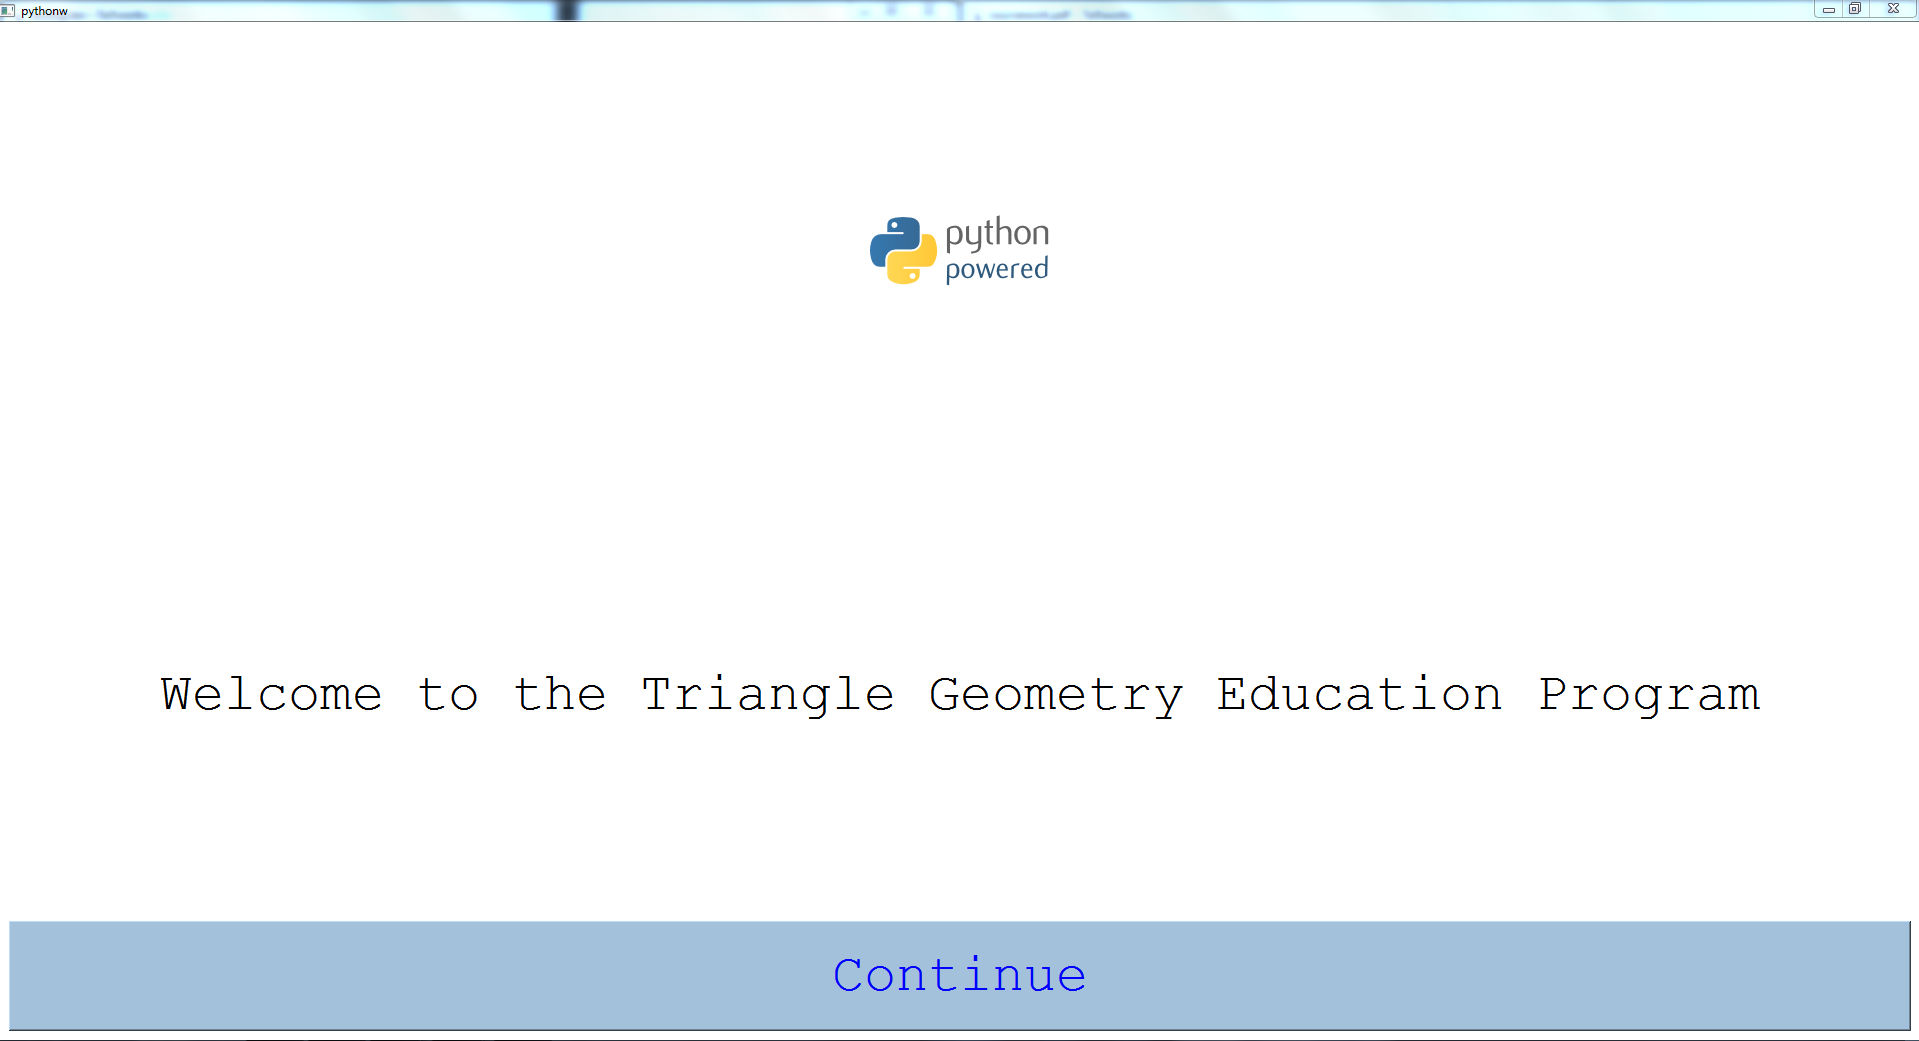
\includegraphics[width=\textwidth]{C:/Users/Jordan/git/COMP4Coursework2/Testing/screen_1}
\end{figure}

This screen is in the first window which opens when the system is run; it contains the title of the system, a picture, and a welcome message for user friendliness, and a continue button is present for switching to the home screen.

\begin{figure}[H]
    \label{fig: Second Screen}\caption{Home Screen}
    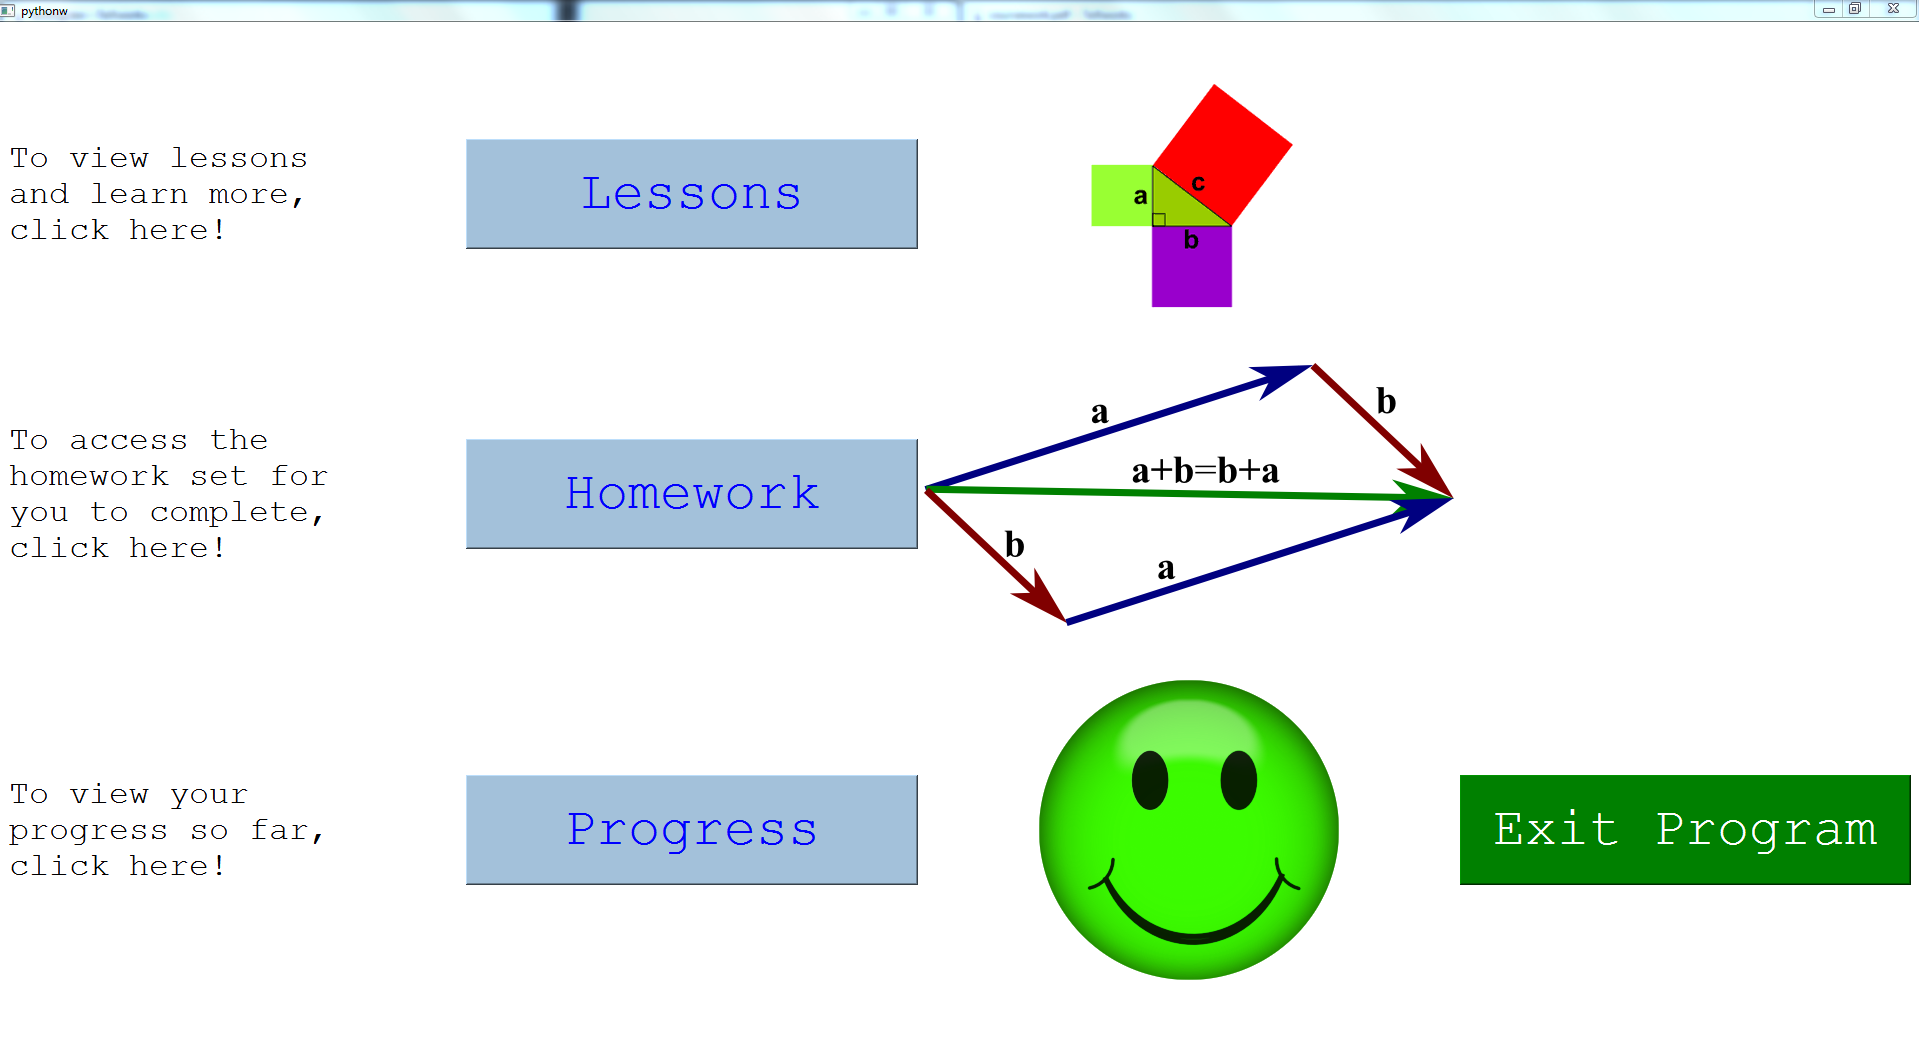
\includegraphics[width=\textwidth]{C:/Users/Jordan/git/COMP4Coursework2/Testing/screen_2}
\end{figure}

This screen is in the same stack window as the first screen and is displayed after the continue button is clicked. It contains four buttons: lessons, homework, progress and exit program, for accessing the lesson topic menu, the homework topic menu, the database viewer and exiting the program respectively. It also contains a picture for each of the three navigation buttons which suggest where the button will take them; they are relevant to the next screens and are user friendly.

\begin{figure}[H]
    \label{fig: Second Screen}\caption{Lesson Topic Menu}
    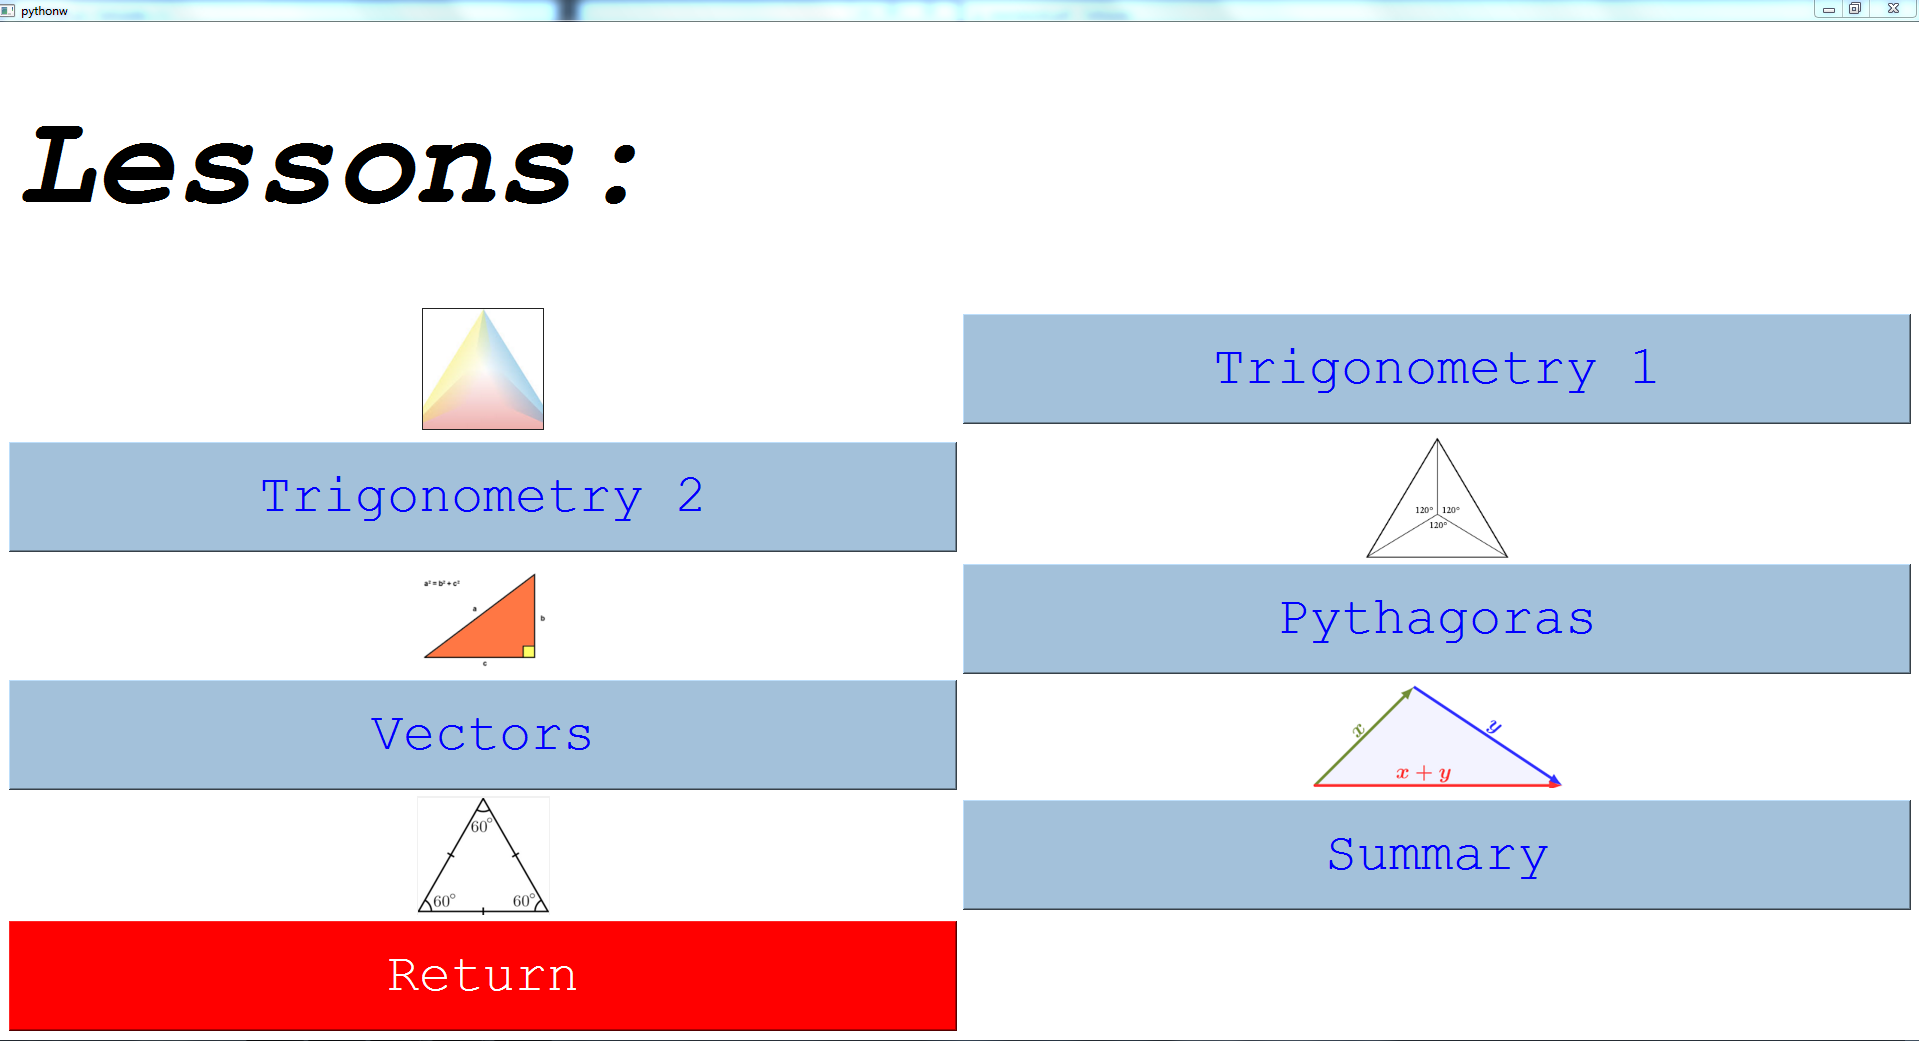
\includegraphics[width=\textwidth]{C:/Users/Jordan/git/COMP4Coursework2/Testing/screen_3}
\end{figure}

This screen is displayed when the user selects the lessons button on the home screen. It contains a title image which tells the user which screen they are on, followed by five buttons, each of which navigate to a topic specific sub-menu (which all appear the same, except for text and images, as they share a parent class). Each button is accompanied by a user friendly picture relevant to the topic menu they lead to. There is a return button which closes the window and returns the user to the home screen.

\begin{figure}[H]
    \label{fig: Second Screen}\caption{Trigonometry 1 Lesson Menu}
    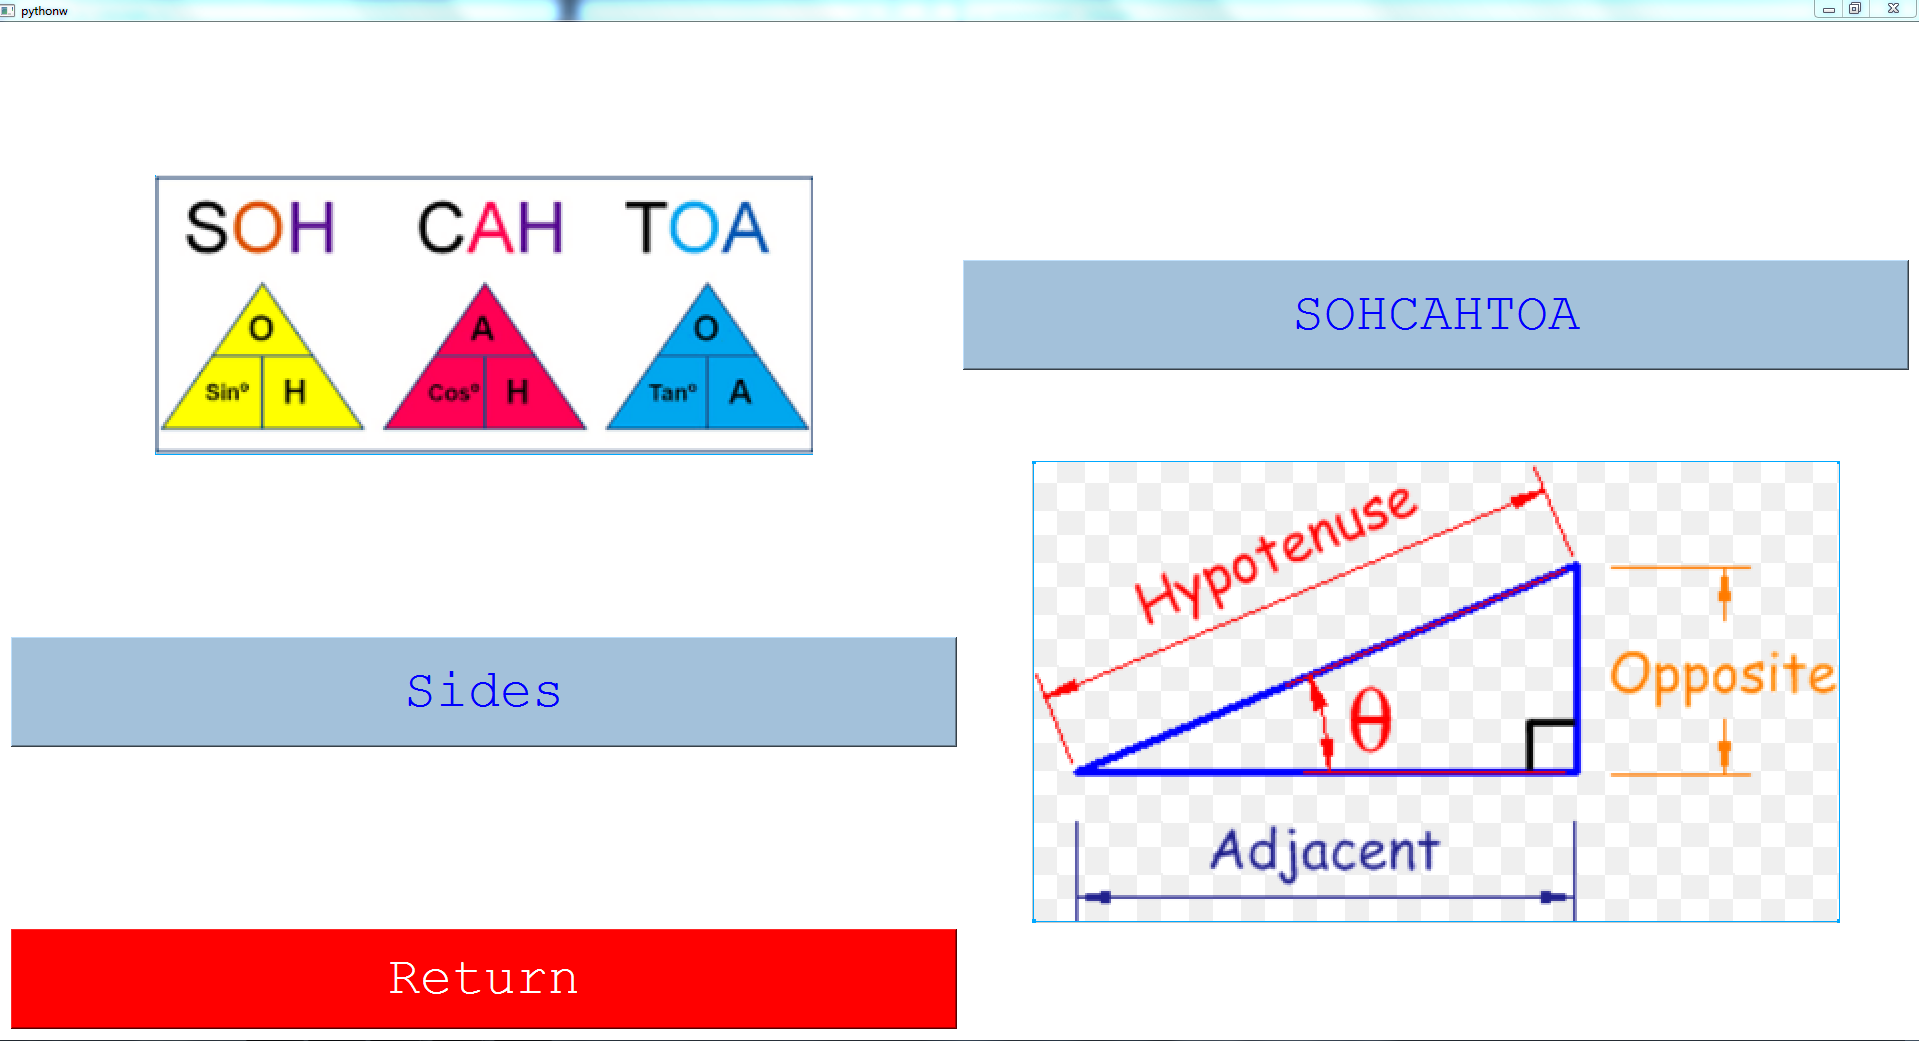
\includegraphics[width=\textwidth]{C:/Users/Jordan/git/COMP4Coursework2/Testing/screen_4}
\end{figure}

This window opens when the user clicks the first button on the lesson topic menu. It is one of five subclasses from the ParentLessonMenu, so these five windows essentially contain the same layout, only with different words, pictures and connections. They each contain a title image which tells the user which screen they are on, and have either two or three buttons, each accompanied by a picture, depending on how many lessons are in the selected topic menu. There is a return button which closes the window and returns the user to the lesson topic menu.

\begin{figure}[H]
    \label{fig: Second Screen}\caption{SOHCAHTOA 1st Lesson screen}
    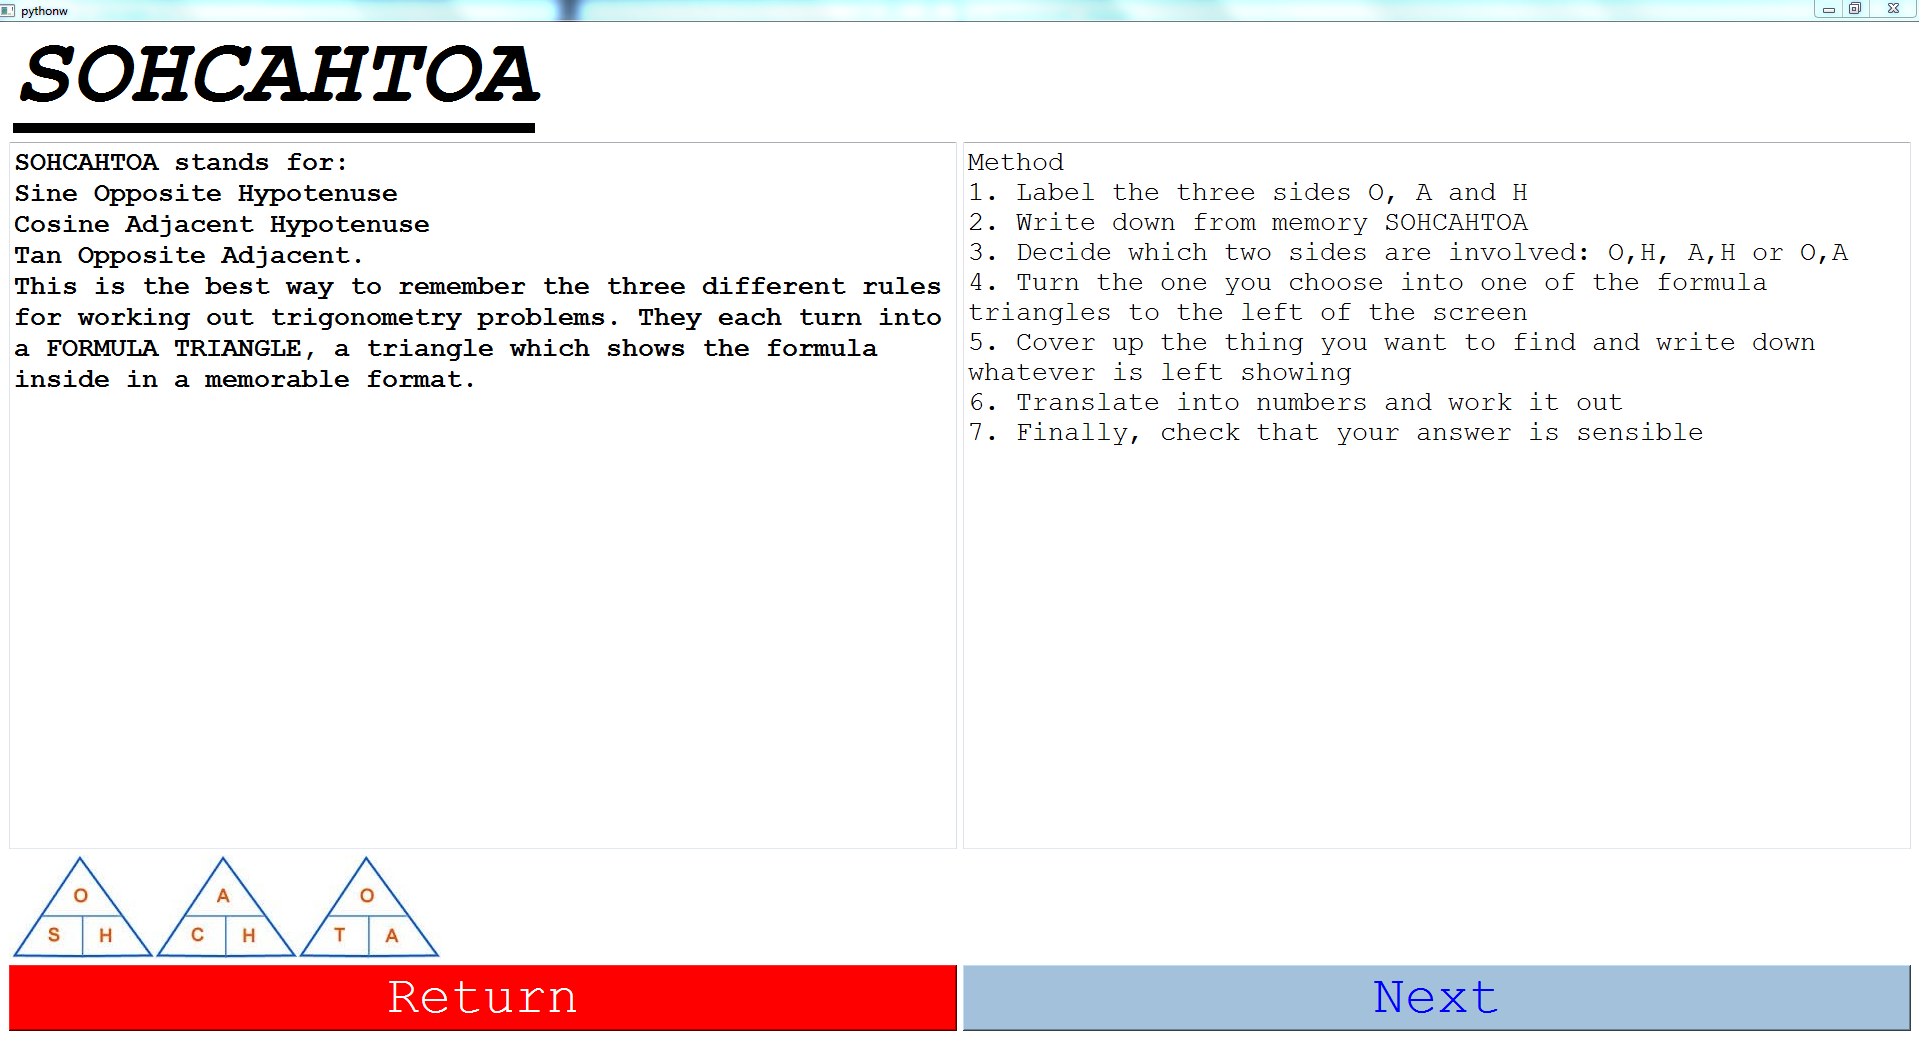
\includegraphics[width=\textwidth]{C:/Users/Jordan/git/COMP4Coursework2/Testing/screen_5}
\end{figure}

This window is accessed by clicking the corresponding button on one of the five derived lesson menus. It is one of nine first lesson's screens which inherit from a parent class; they each contain a title image, two text boxes for lessons and explanations, and cancel button, and a next button, along with one or two images depending on the lesson.

\begin{figure}[H]
    \label{fig: Second Screen}\caption{SOHCAHTOA 2nd Lesson screen}
    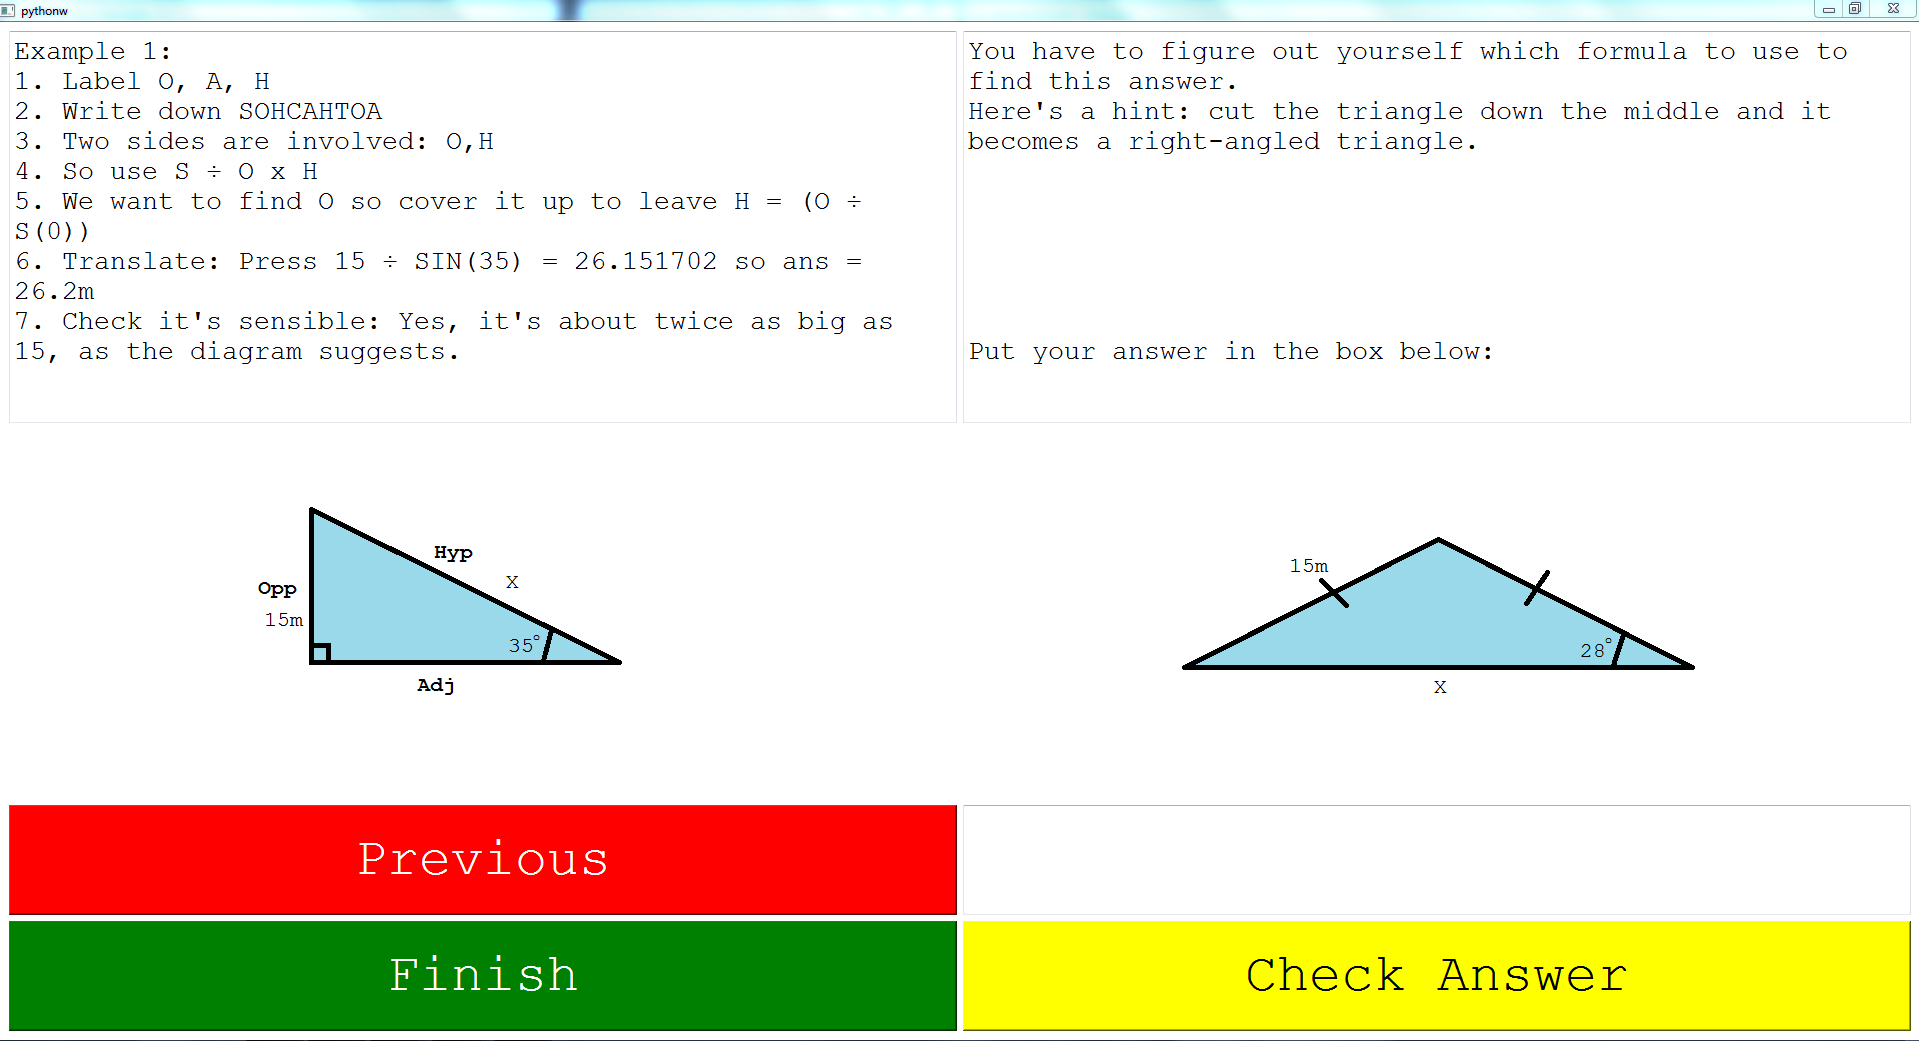
\includegraphics[width=\textwidth]{C:/Users/Jordan/git/COMP4Coursework2/Testing/screen_6}
\end{figure}

This window is in the same stack as the SOHCAHTOA 1st lesson screen, is also sub classed from a parent, and is accessed by clicking the next button. It contains a further two text boxes for lessons and examples, a check button with a line edit for a practice question which you can check the answer to, a previous button to switch back to the first lesson screen, and finish button to close the stack, and one or two images, again, depending on the lesson.

\begin{figure}[H]
    \label{fig: Second Screen}\caption{Homework Topic Menu}
    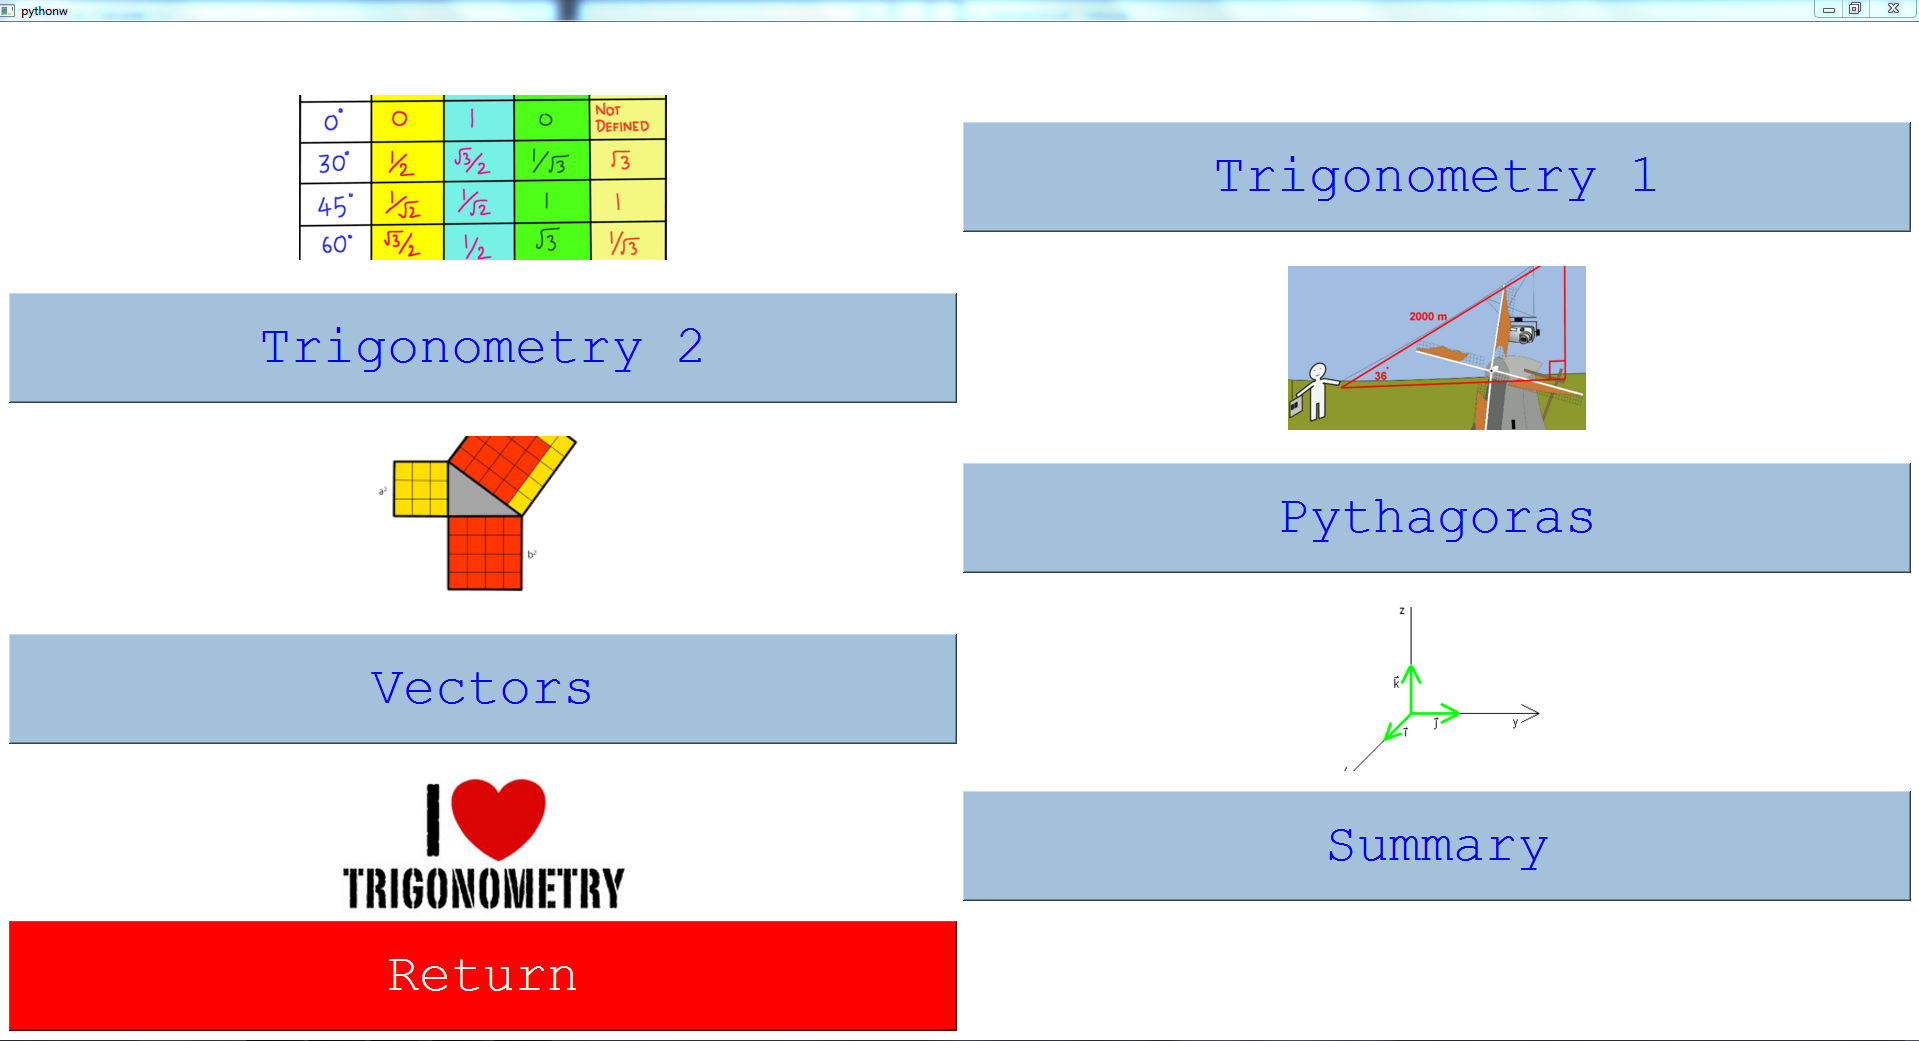
\includegraphics[width=\textwidth]{C:/Users/Jordan/git/COMP4Coursework2/Testing/screen_7}
\end{figure}

This screen is displayed when the user selects the homework button on the home screen. It contains a title image which tells the user which screen they are on, followed by five buttons, each of which navigate to a topic specific sub-menu (which all appear the same, except for text and images, as they share a parent class). Each button is accompanied by a user friendly picture relevant to the topic menu they lead to. There is a return button which closes the window and returns the user to the home screen.

\begin{figure}[H]
    \label{fig: Second Screen}\caption{Trigonometry 1 Homework Menu}
    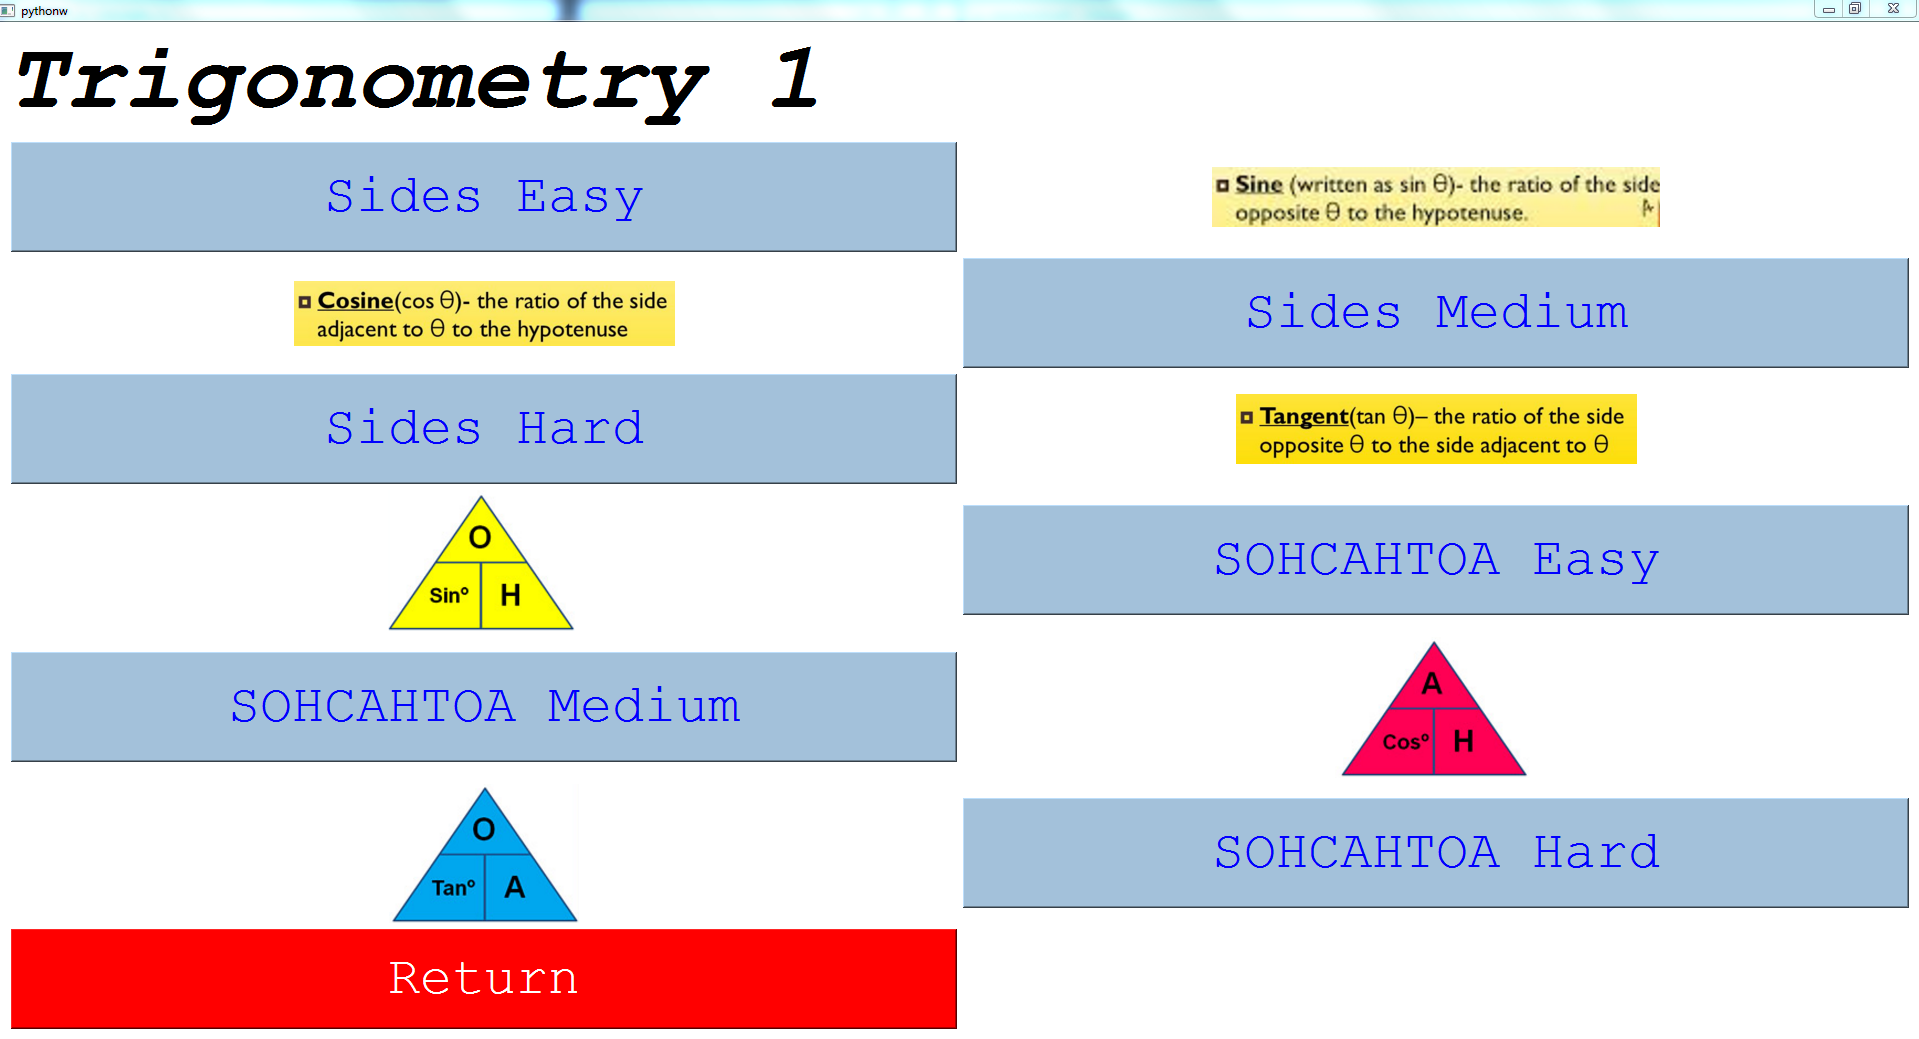
\includegraphics[width=\textwidth]{C:/Users/Jordan/git/COMP4Coursework2/Testing/screen_8}
\end{figure}

This window opens when the user clicks the first button on the homework topic menu. It is one of five subclasses from the HomeworkMenuParentClass, so these five windows essentially contain the same layout, only with different words, pictures and connections. They each contain a title image which tells the user which screen they are on, and have either three or six buttons, each accompanied by a picture, depending on how many homework tasks are in the selected topic menu. There is a return button which closes the window and returns the user to the homework topic menu.

\begin{figure}[H]
    \label{fig: Second Screen}\caption{Sides Easy 1st Homework Screen}
    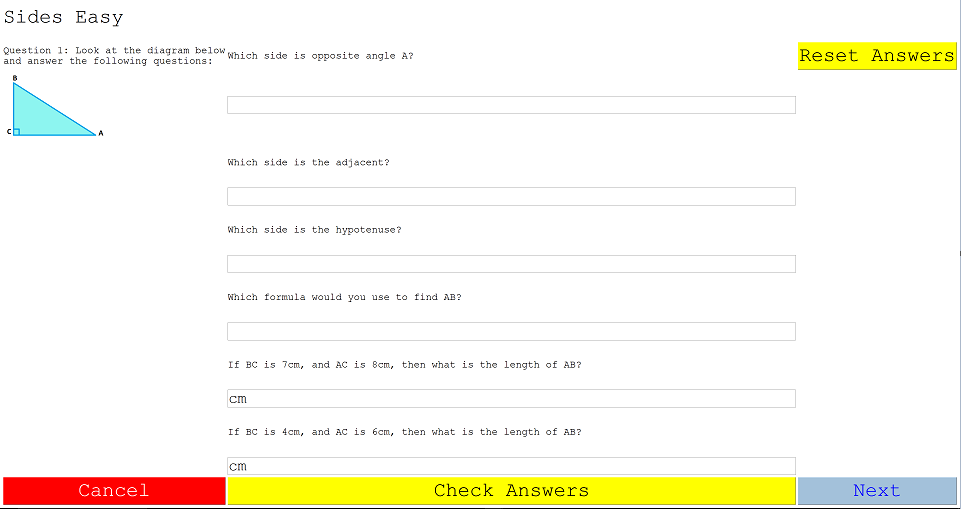
\includegraphics[width=\textwidth]{C:/Users/Jordan/git/COMP4Coursework2/Testing/screen_9}
\end{figure}

This window is accessed by clicking the corresponding button on one of the five derived homework menus. It is one of twenty-seven first homework screens which inherit from a parent class; they each contain a title image, a question, a reset button, a check answers button, a cancel button, a next button, and six line edits into which the user can input their answers to the question, which can be marked using the check button or all cleared using the reset button. 

\begin{figure}[H]
    \label{fig: Second Screen}\caption{Sides Easy 2nd Lesson screen}
    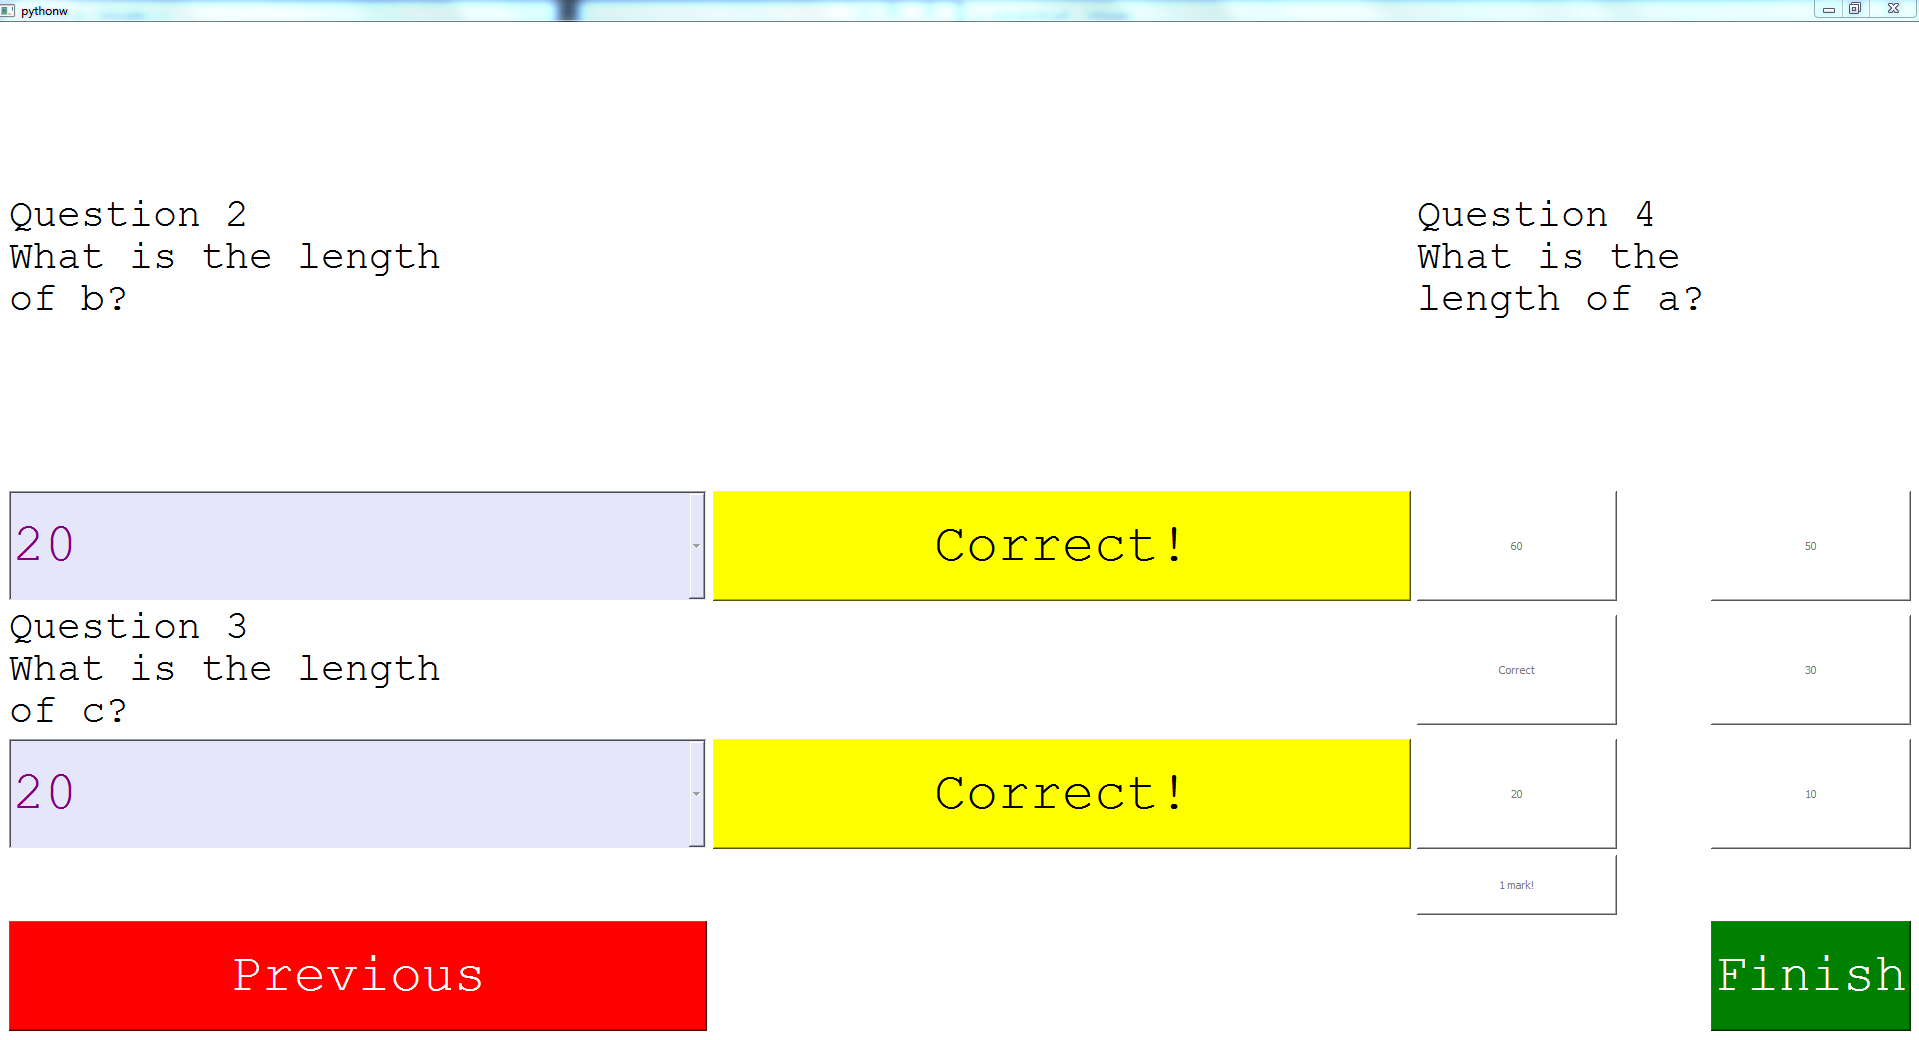
\includegraphics[width=\textwidth]{C:/Users/Jordan/git/COMP4Coursework2/Testing/screen_10}
\end{figure}

This window is in the same stack as the Sides Easy 1st homework screen, is also sub classed from a parent, and is accessed by clicking the next button. It contains three questions as QLabels, two combo boxes, two mark it buttons, six multiple choice buttons, a button showing the remaining number of attempts, a previous button, and a finish button.

\begin{figure}[H]
    \label{fig: Second Screen}\caption{Progress Screen}
    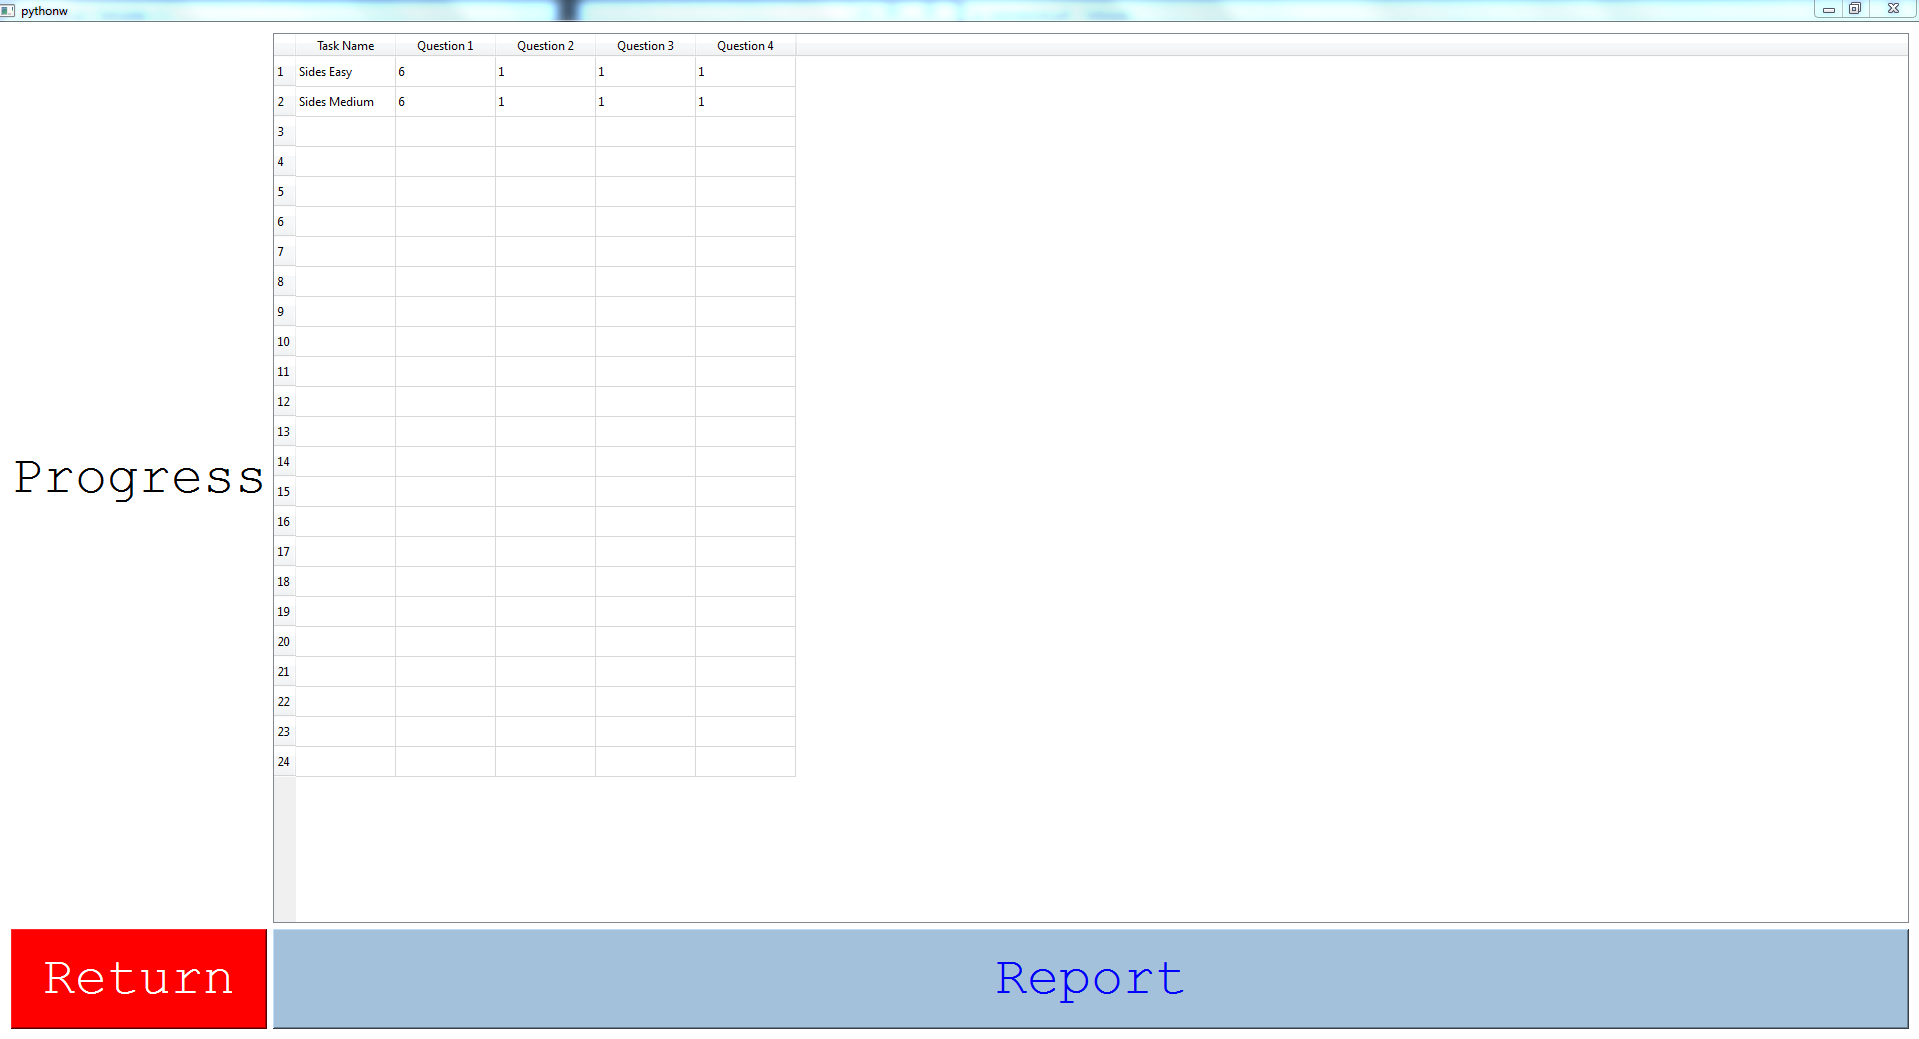
\includegraphics[width=\textwidth]{C:/Users/Jordan/git/COMP4Coursework2/Testing/screen_11}
\end{figure}

This window opens when the user selects progress from the home screen. It contains a title, a return button, a report button, which opens the report widget, and a QTableWidget which contains the data fetched from the database automatically every time the screen is loaded.

\begin{figure}[H]
    \label{fig: Second Screen}\caption{Report Screen}
    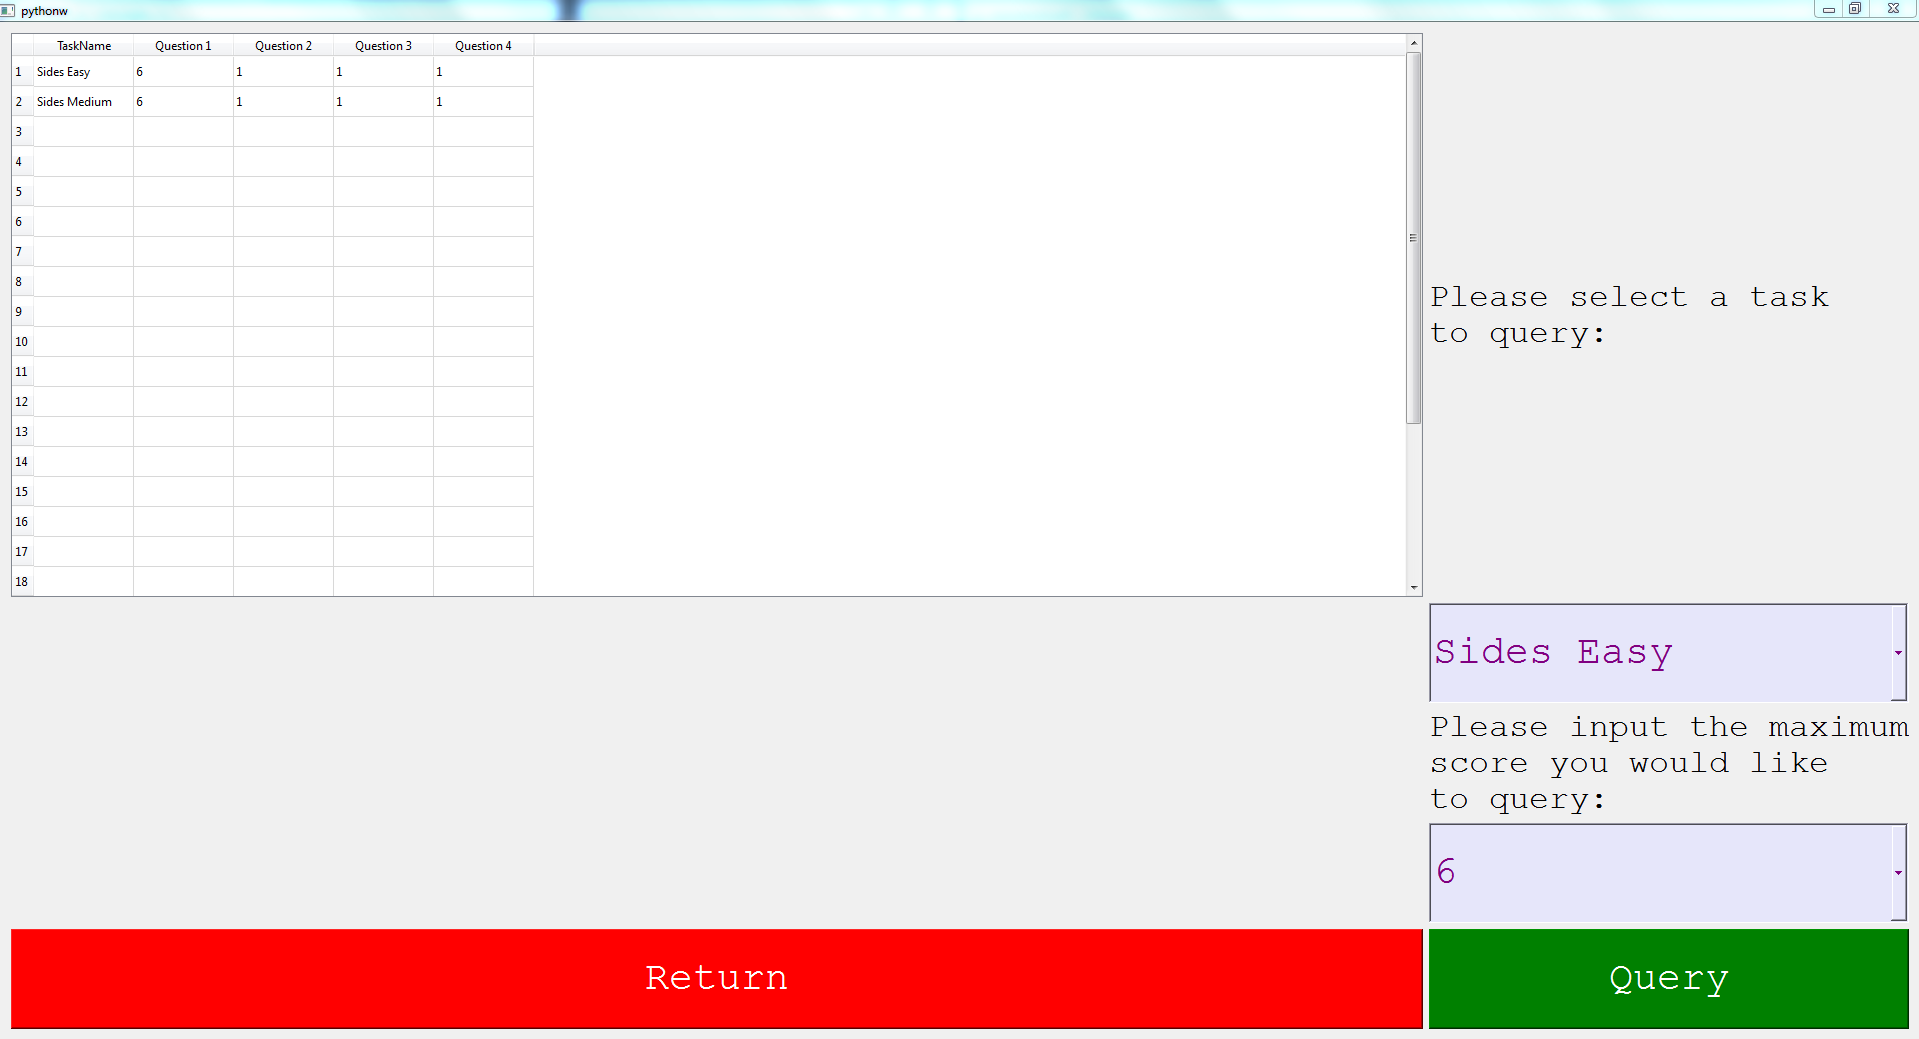
\includegraphics[width=\textwidth]{C:/Users/Jordan/git/COMP4Coursework2/Testing/screen_12}
\end{figure}

This window opens when the user selects report from the progress screen. It contains a QTableWidget which displays the results of the query, a return button, a task combo box, a score combo box and a query button, which are used by the user to input a query for the database.

\subsection{ER Diagram}

\begin{figure}[H]
    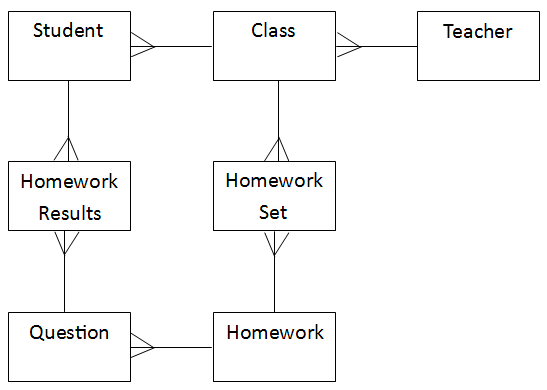
\includegraphics[width=\textwidth]{C:/Users/Jordan/git/COMP4Coursework2/Analysis/er_diagram.png}
    \label{fig:print_function_result}
\end{figure}

\subsection{Class Diagrams}

\begin{center}
\begin{tabular}{|p{7cm}|} \hline
\textbf{MyWindow Class} \\ \hline
NameEntered : Boolean \\
self.login\_widget : Class \\
self.student\_home : Class \\
self.stack : Class \\
self.widget : Class \\ \hline
enter\_program : Boolean \\ \hline
\end{tabular}
\end{center}

\begin{center}
\begin{tabular}{|p{7cm}|} \hline
\textbf{Database Class} \\ \hline
self.\_db\_name : String \\
self.table\_name : String \\ \hline
execute\_sql : String \\
create\_table : String \\
insert\_data\_first : String, Integer \\
insert\_data\_second : String, Integer, Integer, Integer \\
get\_query : String, Integer \\
GetAllNames : \\ \hline
\end{tabular}
\end{center}

\begin{center}
\begin{tabular}{|p{7cm}|} \hline
\textbf{DatabaseWidget Class} \\ \hline
students : List \\
count : Integer \\ \hline
selected\_back : \\
selected\_report : \\ \hline
\end{tabular}
\end{center}

\begin{center}
\begin{tabular}{|p{7cm}|} \hline
\textbf{ParentHomeworkPage1Class} \\ \hline
self.task : String \\
self.allow\_cont : Boolean \\
self.answers : List \\ \hline
check\_selected : \\
next\_selected : \\
reset\_selected : \\
cancel\_selected : \\
open\_page\_2 : \\ \hline
\end{tabular}
\end{center}

\begin{center}
\begin{tabular}{|p{7cm}|} \hline
\textbf{HomeworkPage2ParentClass} \\ \hline
self.task : String \\
self.attempts\_remaining\_a : Integer, Real \\
self.attempts\_remaining\_b : Integer, Real \\
self.attempts\_remaining\_c : Integer, Real \\
self.correct\_count\_2 : Integer, Real \\
self.correct\_count\_3 : Integer, Real \\
self.correct\_count\_4 : Integer, Real \\
self.answer\_question\_4 : Real \\ \hline
check\_button\_1 : Integer, Real \\
check\_button\_2 : Integer, Real \\
check\_button\_3 : Integer, Real \\
check\_button\_4 : Integer, Real \\
check\_button\_5 : Integer, Real \\
check\_button\_6 : Integer, Real \\
selected\_mark\_2 : Integer, Real \\
selected\_mark\_3 : Integer, Real \\
selected\_previous : \\
selected\_finish : \\ \hline
\end{tabular}
\end{center}

\begin{center}
\begin{tabular}{|p{7cm}|} \hline
\textbf{QErrorMessage} \\ \hline
message : String \\ \hline
x.showMessage : String \\ \hline
\end{tabular}
\end{center}

\subsection{Navigation Diagram}

\begin{figure}[H]
    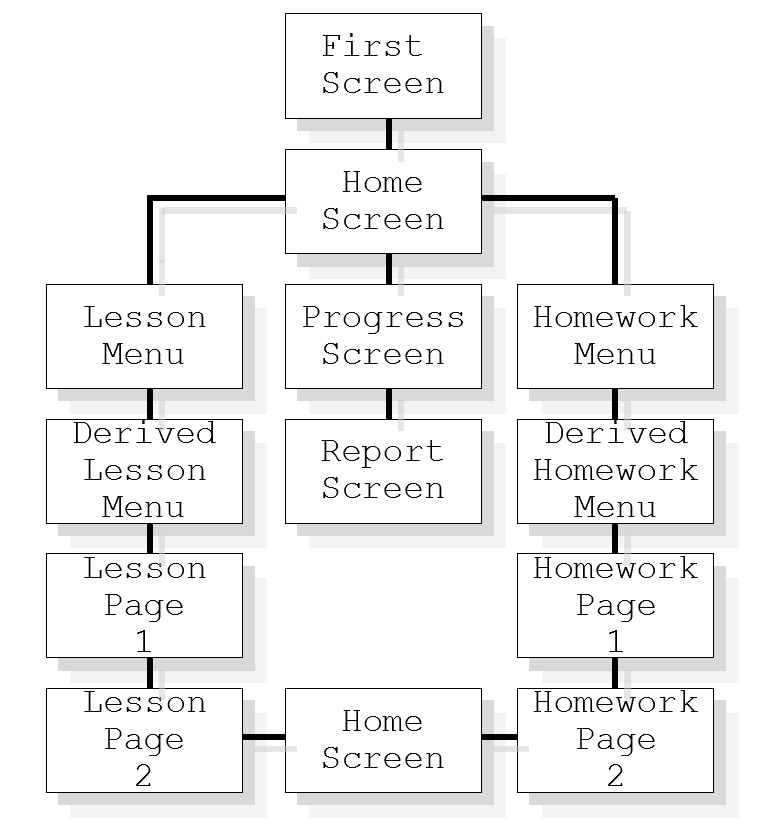
\includegraphics[width=\textwidth]{C:/Users/Jordan/git/COMP4Coursework2/Maintenance/nav_diagram.png}
    \label{fig:print_function_result}
\end{figure}

\subsection{Database Table Views}

\textbf{Task Entity: }

\begin{figure}[H]
    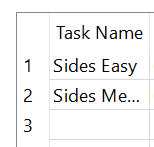
\includegraphics[width=\textwidth]{C:/Users/Jordan/git/COMP4Coursework2/Maintenance/task_db.png}
    \label{fig:print_function_result}
\end{figure}

This is the task name entity where the name of the task hard-coded from the subclass homework has been recorded along with the scores.

\textbf{Qone Entity: }

\begin{figure}[H]
    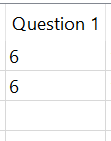
\includegraphics[width=\textwidth]{C:/Users/Jordan/git/COMP4Coursework2/Maintenance/q_one_db.png}
    \label{fig:print_function_result}
\end{figure}

This records the count of the number of correct line edit answers in the subclass for the task.

\textbf{Qtwo Entity: }

\begin{figure}[H]
    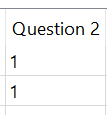
\includegraphics[width=\textwidth]{C:/Users/Jordan/git/COMP4Coursework2/Maintenance/q_two_db.png}
    \label{fig:print_function_result}
\end{figure}

This records the score of the second homework question from each subclass.

\textbf{Qthree Entity: }

\begin{figure}[H]
    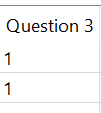
\includegraphics[width=\textwidth]{C:/Users/Jordan/git/COMP4Coursework2/Maintenance/q_three_db.png}
    \label{fig:print_function_result}
\end{figure}

This records the score of the third homework question from each subclass.

\textbf{Qfour Entity: }

\begin{figure}[H]
    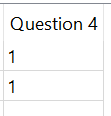
\includegraphics[width=\textwidth]{C:/Users/Jordan/git/COMP4Coursework2/Maintenance/q_four_db.png}
    \label{fig:print_function_result}
\end{figure}

This records the score of the fourth homework question from each subclass.

\textbf{All Entities: }

\begin{figure}[H]
    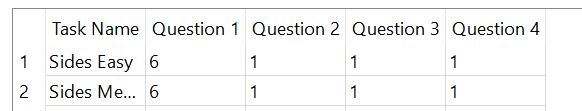
\includegraphics[width=\textwidth]{C:/Users/Jordan/git/COMP4Coursework2/Maintenance/all_db.png}
    \label{fig:print_function_result}
\end{figure}

This shows a whole record for a task that has been saved along with the scores that were obtained on said task.

\subsection{Database SQL}

\textbf{create\_table method: }

\begin{python}
def create_table(self, table_name):
        with sqlite3.connect(self._db_name) as db:
            cursor = db.cursor()
            cursor.execute("select name from sqlite_master where name=?",(table_name,))
            result = cursor.fetchall()
            keep_table = True
            if len(result) == 1:
                response = input("The table {0} already exists, do you wish to recreate it (y/n): ".format(table_name))
                if response == "y":
                    keep_table = False
                    print("The {0} table will be recreated - all existing data will be lost".format(table_name))
                    cursor.execute("drop table if exists {0}".format(table_name))
                    db.commit()
                else:
                    print("The existing table was kept")
            else:
                keep_table = False
            if not keep_table:
                sql = """create table Student
                (TaskID text,
                Qone integer,
                Qtwo integer,
                Qthree integer,
                Qfour integer,
                primary key(TaskID))"""
                cursor.execute(sql)
                db.commit()
\end{python}

This method is responsible for creating the table, and is run whenever the system is run, as it also checks to see if the database already exists before starting. It connects to the database which is identified by the \textit{g\_database} variable which is passed in to the method containing the database file name. The cursor (structure controller) searches all existing database files to see if one named 'Student' (the table\_name variable also passed into the method) already exists. If it does, it asks the user whether or not they want to over-write it; if they input yes, it will the drop the current table and create a new one using the SQL statement at the end of the class. Otherwise, if the boolean keep\_table remains true, the program will just move on; likewise, if the table doesn't already exist, in which the same SQL statement will be used to create it. The SQL statement in this method creates the table called Student, which is the name used to check the database files at the start of the method, and gives the following entities: TaskID, which is the task name and a string, then four question entities which each contain an integer. The SQL here is executed in the same method, rather than the execute\_sql method.

\textbf{Important Database variables: }

\begin{itemize}
	\item self.\_db\_name - This is the name of the database file which is passed into the class when a variable is assigned to it (in this case it is "student\_database.db") and used to identify which database file each SQL method needs to connect to.
	\item self.table\_name - This is the name of the table which is created and is used to check to see if this table already exists, and to identify which table to make changes to when SQL code is executed.
	\item g\_database - This variable is assigned to the database class and given a file name which is passed into the class to be used for identifying the file intended for use.
\end{itemize}

\subsection{SQL Queries}

\subsubsection{create\_table method: }

\begin{python}
"select name from sqlite_master where name=?",(table_name,))
\end{python}

This SQL query takes the name of the table which is being used (Student) and uses it to check the database files to see if a table with that name already exists, so that it can be over-written if need be.

\begin{python}
"drop table if exists {0}".format(table_name))
\end{python}

This SQL query takes the table name (Student) if an existing table with that name is found, and deletes it entirely, if the user chooses to over-write it.

\begin{python}
sql = """create table Student
	(TaskID text,
	Qone integer,
	Qtwo integer,
	Qthree integer,
	Qfour integer,
	primary key(TaskID))"""
\end{python}

This SQL query creates the Student table if it does not already exist; it adds the five entities and then makes TaskID the primary key.

\subsubsection{insert\_data\_first method: }

\begin{python}
"select TaskID from Student where TaskID = '{0}'".format(task))
\end{python}

The task variable, representing the name of the task being completed, is passed through from the first homework screen in use. The SQL statement uses this variable to search the database for any records already existing with the same task name; all records where the task name is the same are fetched and returned to the method in the form of a list variable. If one is found it knows to update rather than create a new record, otherwise it just creates a new record with that task name.

\begin{python}
"UPDATE Student SET Qone = '{0}' WHERE TaskID = '{1}' AND Qone < '{2}'".format(correct_count, task, correct_count)
\end{python}

If a record with the same task name already exists, the update statement is used to record the new correct\_count (score of the first homework question) but only if the new score is better than the old one, checked using the less than symbol. The WHERE part of the statement ensures that the changes are only made to the one record with the same task name rather than all records.

\begin{python}
"insert into Student(TaskID, Qone, Qtwo, Qthree, Qfour) values ('{0}', '{1}', '{2}', '{3}', '{4}')".format(task, correct_count, str(0), str(0), str(0))
\end{python}

This is the insert statement used if a record with the same task name is not found; it saves the task name along with the score of the first homework question, then saves values of 0 in the other three questions entities. This is so that the same update statements can be used in the next method regardless of whether or not a record previously existed, as values are there to be over-written anyway because this method will always be run first due to the access limitations of the second screen (having to submit the first question score before proceeding).

\subsubsection{insert\_data\_second method: }

\begin{python}
"UPDATE Student SET Qtwo = '{0}' WHERE TaskID = '{1}' AND Qtwo < '{2}'".format(count_2, task, count_2)
\end{python}

This SQL statement overwrites the value of the Qtwo entity in the record with the same task name, which will have just been written by the previous method from the first homework screen. If the value already there is less than the new score, then it will be over-written, whether it is a fresh 0 or an existing 4. The count variable is passed through from the second homework screen which calls the method.

\begin{python}
"UPDATE Student SET Qthree = '{0}' WHERE TaskID = '{1}' AND Qthree < '{2}'".format(count_3, task, count_3)
\end{python}

This SQL statement overwrites the value of the Qthree entity in the record with the same task name, which will have just been written by the previous method from the first homework screen. If the value already there is less than the new score, then it will be over-written, whether it is a fresh 0 or an existing 4. The count variable is passed through from the second homework screen which calls the method.

\begin{python}
"UPDATE Student SET Qfour = '{0}' WHERE TaskID = '{1}' AND Qfour < '{2}'".format(count_4, task, count_4)
\end{python}

This SQL statement overwrites the value of the Qfour entity in the record with the same task name, which will have just been written by the previous method from the first homework screen. If the value already there is less than the new score, then it will be over-written, whether it is a fresh 0 or an existing 4. The count variable is passed through from the second homework screen which calls the method.

\subsubsection{get\_query method: }

\begin{python}
"select * from Student WHERE TaskID = '{0}' or Qone = '{1}'".format(data, score_data)
\end{python}

This is used to query the database using variables passed through from the contents of the combo boxes in the report widget, where the user selects which details to query. The SQL statement searches the database for records which exist containing either one of the two variable values passed through, then returns them to a list variable which can be used to display the result.

\subsubsection{GetAllNames method: }

\begin{python}
"select * from Student"
\end{python}

This SQL statement fetches all information currently stored in the database and returns it to be displayed in the progress window using a list variable to call functions.

\section{Testing}

\subsection{Summary of Results}

Throughout the testing stage I had a few manageable issues, and one quite major issue, but all of these I was able to solve without too much trouble. The biggest problem was having to cut out all administrator capabilities from the system, and turn it into a single user program, due to a lack of time and knowledge. However, referring to the parts of the system which I actually created, the system was proven to be both reliable and robust one these problems had been fixed, as there is now no point where an endless loop can be entered or a crash occurs, and all data is stored responsibly. Save the administrator aspects, the system generally meets the user requirements as it is user friendly, easy to use and contains the subject material needed to teach trigonometry using a range of input types.

The problems I encountered includes the following:

\begin{itemize}
	\item The report widget having to be put on the same screen as the query inputs as I could not find a way to pass variables through to a separate pop-up window class
	\item Not having the knowledge to implement a drag and drop system into the homework, and replacing it with a multiple choice button system
	\item Implementing separate accounts with log-ins and access restrictions for an administrator
	\item Being able to save a total score to the database due to not being able to pass the variables through to the same window to be transformed together
	\item The database would not over-write an existing record with the same task name, it would just crash, until I implemented an update SQL statement
	\item The QTableWidgets would only display one record because they kept over-writing in the first row, until I placed a for loop in to increment the row count
\end{itemize}

\textbf{Below is the results table from the testing stage: }

\begin{landscape}

\begin{center}
\begin{longtable}{|p{2.5cm}|p{4cm}|p{4cm}|p{4.5cm}|p{3cm}|} \hline
\textbf{Test Number} & \textbf{Expected Result} & \textbf{Test Data} & \textbf{Actual Result} & \textbf{Screenshot Numbers} \\ \hline
1.003 & The lessons menu should be displayed & Click the lessons button & The lessons menu was displayed, as expected & Figures 3.1, 3.2 \\ \hline
1.004 & The homework menu should be displayed & Click the homework button & The homework menu was displayed, as expected & Figures 3.3, 3.4 \\ \hline
1.005 & The progress window should be displayed & Click the progress button & The progress window was displayed, as expected & Figures 3.5, 3.6 \\ \hline
1.006 & The program should close entirely & Click the exit program button & The entire program closed, as expected & Figures 3.7, 3.8 \\ \hline
1.007 & The Trigonometry 1 lesson menu should be displayed & Click the Trigonometry 1 button & The Trigonometry 1 lesson menu was displayed, as expected & Figures 3.9, 3.10 \\ \hline
1.012 & The lesson menu should be closed and the home screen displayed & Click the return button & The lesson menu closed and the home screen was displayed, as expected & Figures 3.11, 3.12 \\ \hline
1.013 & The SOHCAHTOA first lesson screen should be displayed & Click the SOHCAHTOA button & The SOHCAHTOA first lesson screen was displayed, as expected & Figures 3.13, 3.14 \\ \hline
1.015 & The Trigonometry 1 lesson menu should be closed and the lesson menu displayed & Click the return button & The Trigonometry 1 lesson menu closed and the lesson menu was displayed, as expected & Figures 3.15, 3.16 \\ \hline
1.031 & The SOHCAHTOA first lesson screen should be closed and the Trigonometry 1 lesson menu should be displayed & Click the return button & The SOHCAHTOA first lesson screen was closed and the Trigonometry 1 lesson menu was displayed, as expected & Figures 3.17, 3.18 \\ \hline
1.032 & The SOHCAHTOA second lesson screen should replace the first SOHCAHTOA lesson screen in display & Click the next button & The second SOHCAHTOA lesson screen replaced the first SOHCAHTOA lesson screen, as expected & Figures 3.19, 3.20 \\ \hline
1.033 & The SOHCAHTOA first lesson screen should replace the second SOHCAHTOA lesson screen in display & Click the previous button & The first SOHCAHTOA lesson screen replaced the second SOHCAHTOA lesson screen, as expected & Figures 3.21, 3.22 \\ \hline
1.034 & The input typed in the line edit should be checked and the user told whether they were correct or not & Click the button & The correct answer was registered as correct and the wrong answer was registered as incorrect, as expected & Figures 3.23, 3.24 \\ \hline
1.035 & The stack window with the SOHCAHTOA lesson should close and the Trigonometry 1 lesson menu be displayed & Click the finish button & The SOHCAHTOA lesson stack was closed and the Trigonometry 1 lesson menu was displayed, as expected & Figures 3.25, 3.26 \\ \hline
1.097 & The Trigonometry 1 homework menu should be displayed & Click the trigonometry 1 button & The Trigonometry 1 homework menu was displayed, as expected & Figures 3.27, 3.28 \\ \hline
1.102 & The homework menu should close and the home screen should be displayed & Click the return button & The homework menu closed and the home screen was displayed, as expected & Figures 3.29, 3.30 \\ \hline
1.103 & The first sides easy homework screen should be displayed & Click the sides easy button & The first sides easy homework screen was displayed, as expected & Figures 3.31, 3.32 \\ \hline
1.135 & The sides easy homework stack should close and the trigonometry 1 homework menu displayed & Click the return button & The sides easy homework stack was closed and the trigonometry 1 homework menu was displayed, as expected & Figures 3.33, 3.34 \\ \hline
1.136 & The 6 line edits should be checked and the user told how many were right, and marks given & Click the check answers button & The line edits were checked, correct answers were recognised and incorrect answers were rejected, as expected & Figures 3.35, 3.36 \\ \hline
1.137 & The 6 line edits contents should all be reset to empty & Click the reset button & All 6 line edits were cleared, as expected & Figures 3.37, 3.38 \\ \hline
1.138 & The second sides easy homework screen should replace the first sides easy homework screen in the stack, and the score from the first question should be stored in the database & Click the next button & The second sides easy homework screen replaced the first sides easy homework screen in the stack, and the correct score count was stored in the database, as expected & Figures 3.39, 3.40 \\ \hline
1.139 & The input in the combo box should be checked, the user informed if they are correct or not, and marks be added or attempts removed & Click the mark it button & The correct answer was recognised and marks added, and the incorrect answer recognised and attempts removed afterwards, as expected & Figures 3.41, 3.42 \\ \hline
1.140 & The input in the combo box should be checked, the user informed if they are correct or not, and marks be added or attempts removed & Click the mark it button & The correct answer was recognised and marks added, and the incorrect answer recognised and attempts removed afterwards, as expected & Figures 3.43, 3.44 \\ \hline
1.141 & The correct button should be checked, the user informed if they are correct or not, and marks be added or attempts removed & Click each possible button & The correct answer was recognised and marks added, and the incorrect answer recognised and attempts removed afterwards, as expected & Figures 3.45, 3.46, 3.47 \\ \hline
1.142 & The first sides easy homework screen should replace the second sides easy homework screen in the stack & Click the previous button & The first sides easy homework screen replaced the second sides easy homework screen in the stack, as expected & Figures 3.48, 3.49 \\ \hline
1.143 & the sides easy homework stack should be closed and the home screen should be displayed; The scores from the questions should be stored in the database & Click the finish button & The sides easy homework stack was closed, the home screen was displayed, and the scores were saved to the database, as expected & Figures 3.50, 3.51 \\ \hline
1.380 & The progress screen should be closed and the home screen displayed & Click the return button & The progress screen was closed and the home screen was displayed, as expected & Figures 3.52, 3.53 \\ \hline
1.431 & The report screen should be closed and the progress screen displayed & Click the return button & The report screen was closed and the home screen was displayed, as expected & Figures 3.54, 3.55\\ \hline
1.432 & The relevant information should be fetched from the database and displayed in the same window & Click the query button & Relevant information was found and displayed in the database in the same window, as expected & Figures 3.56, 3.57 \\ \hline
1.441 & The welcome screen should close and the home screen should be displayed & Click the continue button & The welcome screen was closed and the home screen was displayed, as expected & Figures 3.58, 3.59 \\ \hline
1.442 & The report screen should open and the progress screen hidden & Click the report button & The progress screen closed and the report screen was displayed, as expected & Figures 3.60, 3.61 \\ \hline
2.003 & If the input is correct, the word correct should be displayed, otherwise incorrect should be displayed & 5 (or right answer); abc; None & Correct was displayed, incorrect was displayed and an error message for no answer was displayed respectively, as expected & Figures 3.62, 3.63 \\ \hline
2.016 & If the input is correct, the word correct should be displayed, otherwise incorrect should be displayed & 1 (or right answer); abc; None & Correct was displayed, incorrect was displayed and an error message for no answer was displayed respectively, as expected & Figures 3.64, 3.65 \\ \hline
2.017 & If the input is correct, the word correct should be displayed, otherwise incorrect should be displayed & 2 (or right answer); abc; None & Correct was displayed, incorrect was displayed and an error message for no answer was displayed respectively, as expected & Figures 3.64, 3.65 \\ \hline
2.018 & If the input is correct, the word correct should be displayed, otherwise incorrect should be displayed & 3 (or right answer); abc; None & Correct was displayed, incorrect was displayed and an error message for no answer was displayed respectively, as expected & Figures 3.64, 3.65 \\ \hline
2.019 & If the input is correct, the word correct should be displayed, otherwise incorrect should be displayed & 4 (or right answer); abc; None & Correct was displayed, incorrect was displayed and an error message for no answer was displayed respectively, as expected & Figures 3.64, 3.65 \\ \hline
2.020 & If the input is correct, the word correct should be displayed, otherwise incorrect should be displayed & 5 (or right answer); abc; None & Correct was displayed, incorrect was displayed and an error message for no answer was displayed respectively, as expected & Figures 3.64, 3.65 \\ \hline
2.021 & If the input is correct, the word correct should be displayed, otherwise incorrect should be displayed & 6 (or right answer); abc; None & Correct was displayed, incorrect was displayed and an error message for no answer was displayed respectively, as expected & Figures 3.64, 3.65 \\ \hline
2.022 & If the contents of the combo box is correct, correct should appear in the button next to it, otherwise an attempt will be removed & 20; 10 & For the correct answer, correct was printed, an incorrect for the incorrect answer, as expected & Figures 3.66, 3.67 \\ \hline
2.023 & If the contents of the combo box is correct, correct should appear in the button next to it, otherwise an attempt will be removed & 40; 15 & For the correct answer, correct was printed, an incorrect for the incorrect answer, as expected & Figures  3.68, 3.69 \\ \hline
2.024 & If the right button is clicked, display correct, otherwise display incorrect & Each button in order & When the right button was clicked, a mark was added, and when the wrong buttons were clicked attempts were removed, as expected & Figures  3.70, 3.71 \\ \hline
2.295 & The information relevant to the input should be fetched from the database and displayed & Sides Easy; Pythagoras Theorem Hard & The relevant task name was fetched and displayed, as expected & Figure 3.72 \\ \hline 
2.296 & The information relevant to the input should be fetched from the database and displayed & 70\%; 80\% & The relevant scores were fetched and displayed, as expected & Figure 3.73 \\ \hline
3.009 & The task names should be stored under the 'Task Names' header in the database & Complete a task & The task name was stored under 'Task Names', as expected & Figure 3.74 \\ \hline
3.011 & The IndividualPercentScores should be stored under the 'QOne', 'QTwo', 'QThree', and 'QFour' headers respective to the question number in the database & Complete a task & The scores were under their respective headings, as expected & Figure 3.75 \\ \hline
4.015 & The correct output should be displayed for a correct or incorrect or absent input & [Correct answer]; [Incorrect answer]; None & The correct outputs were given, as expected & Figures 3.76, 3.77, 3.78 \\ \hline
4.016 & The correct output should be displayed for a correct or incorrect or absent input & [Correct answer]; [Incorrect answer]; None & The correct outputs were given, as expected & Figures 3.79, 3.80, 3.81 \\ \hline
4.017 & The correct output should be displayed for a correct or incorrect or absent input & [Correct answer]; [Incorrect answer]; None & The correct outputs were given, as expected & Figures 3.82, 3.83, 3.84 \\ \hline
4.018 & The correct output should be displayed for a correct or incorrect or absent input & [Correct answer]; [Incorrect answer]; None & The appropriate outputs were given for every possile input tested & 3.85, 3.86 \\ \hline
5.001 & The client should be satisfied with the overall system & Show the client each aspect of the system & The client believes that 71.9\% of the objectives have been met & See Evaluation Section 6.7 \\ \hline
5.003 & The task names and scores should be being saved to an sqlite database, 5 columns, as many rows as there are tasks & Complete a task & There are the right number of headings in the table all with the correct information being displayed in them, as expected & Figure 3.87 \\ \hline
5.004 & Only the task names and scores should be stored in the database & Complete a task & They are the only pieces of information being stored, as expected & Figure 3.88 \\ \hline
5.006 & No illegitimate information or personal information should be being stored & Complete a task (only source of information for the database) & No illegitimate information or personal information is being stored, only task names and scores, so the DPA cannot be breached anyway & Figure 3.89 \\ \hline
\end{longtable}
\end{center}

\end{landscape}

\subsection{Known Issues}

The only problem remaining is that of the administrator aspect of the system not being possible to create using the time and knowledge I have. In the Python 3.4 shell, every time a window is opened an error to do with the \_raise function pops up, however this does not affect the running of the program in any way and the user will never see this error in the distributed version of the system. Without, this function, the windows will not be displayed, so I cannot simply remove it. Lastly, I will not be able to record total scores from tasks as I still am unable to find a way to pass the appropriate variables through to the appropriate classes.

Otherwise, all of the other problems mentioned in section 3.4.2 have either been solved or replaced with an alternative working solution.

\section{Code Explanations}

\subsection{Difficult Sections}

\textbf{selected\_submit method (ReportWidget Class 4.3.3)}

\begin{python}
def selected_submit(self):
        _count = 0
        data = self.task_box.currentText()
        score_data = self.score_box.currentText()
        report = g_database.get_query(data, score_data)
        for count in range(7):
            self.db.setItem(count, 0, QTableWidgetItem(None))
            self.db.setItem(count, 1, QTableWidgetItem(None))
            self.db.setItem(count, 2, QTableWidgetItem(None))
            self.db.setItem(count, 3, QTableWidgetItem(None))
            self.db.setItem(count, 4, QTableWidgetItem(None))
        for record in report:
            self.db.setItem(_count, 0, QTableWidgetItem(record[0]))
            self.db.setItem(_count, 1, QTableWidgetItem(str(record[1])))
            self.db.setItem(_count, 2, QTableWidgetItem(str(record[2])))
            self.db.setItem(_count, 3, QTableWidgetItem(str(record[3])))
            self.db.setItem(_count, 4, QTableWidgetItem(str(record[4])))
            _count += 1
\end{python}

The part where the database method fetches from the database worked fine here, the problem was displaying the data in the QTableWidget in the report window. Only one record would be displayed, and at first I thought it was because the SQL kept over-writing the previous record, and that the fault was with the insert statements. However, it turned out to be to do with the formatting of the fetched information in the QTableWidget; I had to fiddle with counts and tried putting them in different places before all of the data would be displayed, then had to do it again to clear the table with each new query. Eventually the data was all displayed on each row, fixed by an incrementing row count. 

\textbf{Makes the background white (all PyQt classes)}

\begin{python}
pal = QPalette()
        pal.setColor(QPalette.Background, Qt.white)
        self.setAutoFillBackground(True)
        self.setPalette(pal)
\end{python}

This section of simple PyQt code was very hard to come across. I had to research how to change the background colour of a PyQt window on the internet as I had no experience beforehand in this area of PyQt. A very long time was spent trying out similar code which actually only changed the colour of the widgets on the layout rather than the background of the entire window itself. In fact, often everything but the part I wanted to change colour would actually change colour. Eventually, I tried this section of code, and it finally worked, and is useful because I can stick it in parent classes a few times and it will be in all of the subclasses, making the background colour consistent.

\textbf{next\_selected method (ParentHomeworkPage1Class 4.3.18)}

\begin{python}
def next_selected(self):
        cont = False
        while not cont:
            for a in self.answers:
                if a.text() == "":
                    error_message = ErrorMessage8()
                    error_message.show()
                    error_message._raise()
                    cont = False
            cont = True
            if self.allow_cont:
                g_database.insert_data_first(self.task, self.correct_count)
                self.open_page_2()
                self.hide()
            else:
                error_message_2 = ErrorMessage8()
                error_message_2.show()
                error_message_2._raise()
\end{python}

With this method, it was difficult to find the right indentation for the error messages to work with the intended logic, and also change the cont boolean to true. After lots of dry running I managed to get the error messages opening at the right times and the database method to work at the right time.

\textbf{insert\_data\_first method (DatabaseClass 4.3.1)}

\begin{python}
def insert_data_first(self, task, correct_count):
        with sqlite3.connect(self._db_name) as db:
            cursor = db.cursor()
            cursor.execute("select TaskID from Student where TaskID = '{0}'".format(task))
            info = cursor.fetchall()
            if len(info) != 0:
                sql = "UPDATE Student SET Qone = '{0}' WHERE TaskID = '{1}' AND Qone < '{2}'".format(correct_count, task, correct_count)
            else:
                sql = "insert into Student(TaskID, Qone, Qtwo, Qthree, Qfour) values ('{0}', '{1}', '{2}', '{3}', '{4}')".format(task, correct_count, str(0), str(0), str(0))
            self.execute_sql(sql)
\end{python}

I had a large issue with getting the insert\_data\_second method to be able to update and add new values in a record which already existed with no values in some of the entities. I decided to just add 0 values, as technically this would always be true for the user's score until they completed the second page anyway, and it would prove convenient when adding the update statements to the insert\_data\_second method, which would be able to update over 0 values or existing 1, 2, 3 etc. values. It did however take a long time to find this solution.

\textbf{selected\_mark\_2 method (HomeworkPage2ParentClass (4.3.19)}

\begin{python}
def selected_mark_2(self, attempts_remaining_a):
        self.correct_count_2 = 0
        if self.answer_2.currentText() == "20":
            self.correct_count_2 += 1
            self.mark_2.setText("Correct!")
            self.mark_2.setEnabled(False)
            self.answer_2.setEnabled(False)
        else:
            self.attempts_remaining_a -= 1
            self.mark_2.setText("Mark it|{0}".format(self.attempts_remaining_a))
            if self.attempts_remaining_a == 0:
                self.mark_2.setEnabled(False)
                self.answer_2.setEnabled(False)
            error_message = ErrorMessage5()
            error_message.show()
            error_message._raise()
        return self.attempts_remaining_a, self.correct_count_2
\end{python}

It was quite difficult to find the right indentation for the input widget disabling lines of code here. There were quite a few different things too juggle and maintain logic with this check algorithm - for example, counting the number of attempts remaining and only when that reaches 0 actually disabling the right widgets, and popping the error messages at the right time as well. It took a bit of playing around with the indentation but it eventually worked as intended.

\subsection{Self-created Algorithms}

\textbf{insert\_data\_first method (Database Class 4.3.1)}

\begin{python}
    def insert_data_first(self, task, correct_count):
        with sqlite3.connect(self._db_name) as db:
            cursor = db.cursor()
            cursor.execute("select TaskID from Student where TaskID = '{0}'".format(task))
            info = cursor.fetchall()
            if len(info) != 0:
                sql = "UPDATE Student SET Qone = '{0}' WHERE TaskID = '{1}' AND Qone < '{2}'".format(correct_count, task, correct_count)
            else:
                sql = "insert into Student(TaskID, Qone, Qtwo, Qthree, Qfour) values ('{0}', '{1}', '{2}', '{3}', '{4}')".format(task, correct_count, str(0), str(0), str(0))
            self.execute_sql(sql)
\end{python}

1 - The variables which represent the task name and the score the user achieved from a homework first page task are passed into the method.
2 - The database file intended for use, "student\_database.db", is connected to by the controller.
3 - The cursor variable is the structure controller for the database.
4 - This SQL statement searches the database for a record with the same task name as the value being passed through as task.
5 - The data retrieved from the SQL statement is assigned to a list variable.
6 - If a record with the same task name is found, the algorithm will proceed to update it.
7 - This SQL statement updates the value of the Qone entity if the new value is greater than the old one. Otherwise it is just left.
8 - If a record is not found the algorithm will proceed to make a new one.
9 - This SQL statement inserts a new record into the Student table and applies a value to all entities so the next SQL statement can always be an update statement.
10 - The execute\_sql method is run which contains the code which applies the SQL changes to the Student table in the database file.

\textbf{insert\_data\_second method (Database Class 4.3.1)}

\begin{python}
    def insert_data_second(self, task, count_2, count_3, count_4):
        with sqlite3.connect(self._db_name) as db:
            sql = "UPDATE Student SET Qtwo = '{0}' WHERE TaskID = '{1}' AND Qtwo < '{2}'".format(count_2, task, count_2)
            self.execute_sql(sql)
            sql_2 = "UPDATE Student SET Qthree = '{0}' WHERE TaskID = '{1}' AND Qthree < '{2}'".format(count_3, task, count_3)
            self.execute_sql(sql_2)
            sql_3 = "UPDATE Student SET Qfour = '{0}' WHERE TaskID = '{1}' AND Qfour < '{2}'".format(count_4, task, count_4)
            self.execute_sql(sql_3)
\end{python}

1 - The variables representing the scores the user achieved from a homework second page task are passed into the method.
2 - The database file intended for use, "student\_database.db", is connected to by the controller.
3 - This SQL statement takes the score from question 2 and updates either the clean 0 value or the previously obtained lower score of the Qtwo entity.
4 - The execute\_sql method is run which contains the code which applies the SQL changes to the Student table in the database file.
5 - This SQL statement takes the score from question 3 and updates either the clean 0 value or the previously obtained lower score of the Qtwo entity.
6 - The execute\_sql method is run which contains the code which applies the SQL changes to the Student table in the database file.
7 - This SQL statement takes the score from question 4 and updates either the clean 0 value or the previously obtained lower score of the Qtwo entity.
8 - The execute\_sql method is run which contains the code which applies the SQL changes to the Student table in the database file.

\textbf{selected\_submit method (Reportwidget 4.3.3)}

\begin{python}
def selected_submit(self):
        _count = 0
        data = self.task_box.currentText()
        score_data = self.score_box.currentText()
        report = g_database.get_query(data, score_data)
        for count in range(27):
            self.db.setItem(count, 0, QTableWidgetItem(None))
            self.db.setItem(count, 1, QTableWidgetItem(None))
            self.db.setItem(count, 2, QTableWidgetItem(None))
            self.db.setItem(count, 3, QTableWidgetItem(None))
            self.db.setItem(count, 4, QTableWidgetItem(None))
        for record in report:
            self.db.setItem(_count, 0, QTableWidgetItem(record[0]))
            self.db.setItem(_count, 1, QTableWidgetItem(str(record[1])))
            self.db.setItem(_count, 2, QTableWidgetItem(str(record[2])))
            self.db.setItem(_count, 3, QTableWidgetItem(str(record[3])))
            self.db.setItem(_count, 4, QTableWidgetItem(str(record[4])))
            _count += 1
\end{python}

2 - A stepper variable is added to increment the row count for displaying the data in the QTableWidget.
3 - The contents of the task QComboBox is assigned to a variable which can be passed into the get\_query method.
4 - The contents of the score QComboBox is assigned to a variable which can be passed into the get\_query method.
5 - A list variable is assigned to the data which will be returned from the get\_query method.
6 - A for loop is used to clear all values in the QTableWidget, which will only have twenty-seven rows, one for each possible task that could be recorded.
7 - The value none is set for each space in the QTableWidget, removing all values from it.
12 - For every record fetched from the database, a for loop is used to add each record to the QTableWidget.
13 - The \_count stepper variable is used to increment the row count so that each record is displayed on the next row rather than constantly over-writing the first row.
18 - The stepper variable increments.

\textbf{check\_selected method (ParentLessonPage2 4.3.14)}

\begin{python}
def check_selected(self):
        if self.answer.text() == self.answer_lesson:
            self.answer.setText("{0} Correct".format(self.answer_lesson))
        else:
            self.answer.setText("Incorrect")
        self.answer.setReadOnly(True)
        self.check.setEnabled(False)
\end{python}

2 - The algorithm checks to see if the contents of the line edit, i.e. the user's input, is the same as the hard-coded answer in the subclass lesson being used. If it is, it proceeds to tell the user they are correct, whilst leaving their input how it was (3).
4 - If they are not correct, it tells the user they are incorrect (5) and removes their wrong input.
6 - Disables the line edit so the user can no longer enter an input as they are already wrong and have been told the answer.
7 - Disables the check button so they cannot re-check the line edit which will now contain the text "Incorrect", which obviously won't change anyway.

\textbf{check\_selected method (ParentHomeworkPage1Class (4.3.18)}

\begin{python}
def check_selected(self):
        self.allow_cont = False
        self.correct_count = 0
        if self.answer_a.text() == self.answer_1_a:
            self.answer_a.setText("{0} Correct".format(self.answer_a.text()))
            self.correct_count += 1
        else:
            self.answer_a.setText("Incorrect")
        if self.answer_b.text() == self.answer_1_b:
            self.answer_b.setText("{0} Correct".format(self.answer_b.text()))
            self.correct_count += 1
        else:
            self.answer_b.setText("Incorrect")
        if self.answer_c.text() == self.answer_1_c:
            self.answer_c.setText("{0} Correct".format(self.answer_c.text()))
            self.correct_count += 1
        else:
            self.answer_c.setText("Incorrect")
        if self.answer_d.text() == self.answer_1_d:
            self.answer_d.setText("{0} Correct".format(self.answer_d.text()))
            self.correct_count += 1
        else:
            self.answer_d.setText("Incorrect")
        if self.answer_e.text() == self.answer_1_e:
            self.answer_e.setText("{0} Correct".format(self.answer_e.text()))
            self.correct_count += 1
        else:
            self.answer_e.setText("Incorrect")
        if self.answer_f.text() == self.answer_1_f:
            self.answer_f.setText("{0} Correct".format(self.answer_f.text()))
            self.correct_count += 1
        else:
            self.answer_f.setText("Incorrect")
        for a in self.answers:
            a.setReadOnly(True)
        self.check.setEnabled(False)
        self.reset.setEnabled(False)
        self.allow_cont = True
\end{python}

2 - Sets a boolean variable which determines whether or not the system will switch to the next screen based on whether or not the questions have all been answered.
3 - Sets a counter variable to keep track of how many of the line edit user inputs are correct.
4 - Checks to see of the contents of the first line edit, i.e. the user's input, is the same as the hard-coded answer in the homework subclass.
5 - If the input is correct, the user is told they are correct and a mark is awarded.
6 - The counter representing the number of marks is incremented.
7 - If the user input is wrong, the user is told they are wrong (8).
34 - Each line edit is in a list so the code used to change all of them the same way is only written once. A for loop is used for this.
35 - Each line edit is disabled so the user can no longer change their answer.
36 - The check button is disabled so they can't check either their right answer, which would then be interpreted as incorrect due to the additional text, or their wrong answer which would just keep printing "Incorrect" anyway.
37 - The reset button is disabled so they cannot reset all of the right answers or the incorrect messages as they have run out of attempts.
38 - Now that all of the answers have been checked, whether they were right or not, the allow\_cont boolean is changed to true to allow the user to continue to the next screen.

\textbf{next\_selected method (ParentHomeworkPage1Class 4.3.18)}

\begin{python}
def next_selected(self):
        cont = False
        while not cont:
            for a in self.answers:
                if a.text() == "":
                    error_message = ErrorMessage8()
                    error_message.show()
                    error_message._raise()
                    cont = False
            cont = True
            if self.allow_cont:
                g_database.insert_data_first(self.task, self.correct_count)
                self.open_page_2()
                self.hide()
            else:
                error_message_2 = ErrorMessage8()
                error_message_2.show()
                error_message_2._raise()
\end{python}

2 - A boolean variable is set which determines whether or not the system will switch screen based on whether or not the questions have all been answered.
3 - While the boolean is false, the algorithm will proceed to check if the line edit is blank, for each of the six line edits in the list (4, 5)
6 - If a line edit is blank, an error message will appear, and the algorithm will stop and allow the user to input an answer.
9 - The cont boolean remains false.
10 - If none of the line edits are blank, that means they have all been checked and the screen can switch.
11 - If the boolean variable from the check method is true, the insert\_data\_first method is run, saving the scores of the task as a record (12).
13 - The second screen in the stack is displayed.
15 - If the check method has not been run and the line edits have not been checked, it won't allow the user to proceed until they give an input.
16 - An error message is displayed asking the user to finish the questions.

\textbf{reset\_selected method (ParentHomeworkPage1Class 4.3.18)}

\begin{python}
def reset_selected(self):
        self.answer_a.setText(None)
        self.answer_b.setText(None)
        self.answer_c.setText(None)
        self.answer_d.setText(None)
        self.answer_e.setText(None)
        self.answer_f.setText(None)
\end{python}

2 - Simply sets the value of each line edit to none, effectively resetting the question so the user doesn't have to manually delete each input.

\textbf{check\_button\_1 method (HomeworkPage2ParentClass 4.3.19)}

\begin{python}
def check_button_1(self, attempts_remaining_c):
        self.correct_count_4 = 0
        if self._button_1.text() == self.answer_question_4:
            self._button_1.setText("Correct")
            self._button_1.setEnabled(False)
            self._button_2.setEnabled(False)
            self._button_3.setEnabled(False)
            self._button_4.setEnabled(False)
            self._button_5.setEnabled(False)
            self._button_6.setEnabled(False)
            self.attempts_button.setText("1 mark!")
            self.correct_count_4 += 1
        else:
            self._button_1.setText("Incorrect")
            self._button_1.setEnabled(False)
            self.attempts_remaining_c -= 1
            self.attempts_button.setText("{0} attempts remaining".format(self.attempts_remaining_c))
            if self.attempts_remaining_c == 0:
                self._button_1.setEnabled(False)
                self._button_2.setEnabled(False)
                self._button_3.setEnabled(False)
                self._button_4.setEnabled(False)
                self._button_5.setEnabled(False)
                self._button_6.setEnabled(False)
                self.attempts_button.setText("No more attempts")
            return self.attempts_remaining_c
\end{python}

1 - The variable representing the number of attempts the user has left is passed through - This is so that the number doesn't reset if one of the other five methods for the other buttons is run (couldn't be sub classed) and it isn't in the method itself as that would effectively require it to be reset with every click.
2 - The variable representing the user's score is in the method because it needs to be reset every time it is run otherwise it would just accumulate beyond a reasonable value.
3 - Checks to see if the text on the button is the same as the hard-coded answer in the homework subclass.
4 - If it is, it tells the user they are correct.
5 - All the buttons are disabled as they are no longer needed for input.
11 - The user is informed of their score.
12 - The user has a mark added.
13 - If the button text is not the same, the user is told they are incorrect (14).
15 - The incorrect button is disabled so they can't choose the same one again.
16 - The user loses an attempt.
17 - The button displaying the number of attempts the user has left is updated.
18 - If the user has no attempts left (attempts\_remaining reaches 0), all of the multiple choice buttons are disabled (19).
25 - The button displaying the number of attempts the user has left is updated.
26 - The variable representing the number of attempts remaining is returned to be used in the check method for the other five buttons.

\textbf{selected\_mark\_2 method (HomeworkPage2ParentClass 4.3.19)}

\begin{python}
def selected_mark_2(self, attempts_remaining_a):
        self.correct_count_2 = 0
        if self.answer_2.currentText() == self.answer_q_2:
            self.correct_count_2 += 1
            self.mark_2.setText("Correct!")
            self.mark_2.setEnabled(False)
            self.answer_2.setEnabled(False)
        else:
            self.attempts_remaining_a -= 1
            self.mark_2.setText("Mark it|{0}".format(self.attempts_remaining_a))
            if self.attempts_remaining_a == 0:
                self.mark_2.setEnabled(False)
                self.answer_2.setEnabled(False)
            error_message = ErrorMessage5()
            error_message.show()
            error_message._raise()
        return self.attempts_remaining_a, self.correct_count_2
\end{python}

1 - The number representing the number of attempts the user has remaining is passed through so it isn't reset every time the method is run as it would if the variable was in the method.
2 - The correct\_count variable counts the users score.
3 - Checks to see if the value of the text in the QComboBox is the same as the hard-coded answer in the homework subclass.
4 - If it is the same, the user receives a mark.
5 - The user is told they are correct.
6 - The check button is disabled so they cannot exploit marks.
7 - The QComboBox is disabled so they cannot change their input.
8 - If the answer is not correct, the user loses an attempt (9).
10 - The text on the button which has the number or attempts remaining is updated.
11 - If the user has no attempts left, all of the inputs are disabled (12, 13).
14 - An error message tells the user they are wrong regardless of how many attempts they have left.
17 - The attempts\_remaining is returned so it doesn't reset and is the same if the method is run again. The correct\_count is returned to be passed into the insert\_data\_second method to be recorded in the database.

\textbf{selected\_finish method (HomeworkPage2ParentClass 4.3.19)}

\begin{python}
def selected_finish(self):
        if self.attempts_button.text() != "1 mark!" and self.attempts_button.text() != "No more attempts":
            error_message_2 = ErrorMessage8()
            error_message_2.show()
            error_message_2._raise()
        elif self.mark_2.text() != "Correct!" and self.mark_2.text() != "Mark it|0":
            error_message_2 = ErrorMessage8()
            error_message_2.show()
            error_message_2._raise()
        elif self.mark_3.text() != "Correct!" and self.mark_3.text() != "Mark it|0":
            error_message_2 = ErrorMessage8()
            error_message_2.show()
            error_message_2._raise()
        else:
            g_database.insert_data_second(self.task, self.correct_count_2, self.correct_count_3, self.correct_count_4)
            self.parent.close()
\end{python}

2 - If the text of the attempts button displays neither of the texts it would display had the user used all of their attempts, it pops an error (3) as this means they have not answered the question or lost all of their attempts. The same goes for the other two questions.
14 - If all of the buttons have the text which signify that the questions have been properly answered, then the system proceeds to save the records to the database.
16 - The stack widget closes and the user is returned to the home screen.

\section{Settings}

There are no settings which the user or maintainer needs to be aware of; only Python 3 or later, and PyQt4 need to be installed on the computer for the entire program to run with no errors. Nothing will need to be changed or installed in order to develop additional content for the system in patches. Any changes that could possibly be made to this system would be possible using Python 3 and PyQt4. Anything using another software package would likely void some of the client's requirements.

\section{Acknowledgements}

\subsection{Pictures}

\begin{itemize}
	\item \url{https://www.python.org/community/logos/} - Python Powered Logo - First Screen
	\item \url{https://www.mathsisfun.com/Pythagoras.html} - Pythagoras Picture - Home Screen
	\item \url{http://mathinsight.org/vector_introduction} - Vector Picture - Home Screen
	\item \url{http://www.clipartpanda.com/categories/green-smiley-face-png} - Green Face - Home Screen
	\item \url{https://commons.wikimedia.org/wiki/File:Triangle_model_of_love.png} - 1st Triangle - Lesson Topic Menu
	\item \url{https://en.wikipedia.org/wiki/Equilateral_triangle} - 2nd Triangle - Lesson Topic Menu
	\item \url{http://www.bbc.co.uk/bitesize/standard/maths_i/measure/Pythagoras/revision/1/} - 3rd Triangle - Lesson Topic Menu
	\item \url{https://en.wikipedia.org/wiki/Triangle_inequality} - 4th Triangle - Lesson Topic Menu
	\item \url{https://en.wikipedia.org/wiki/Equilateral_triangle} - 5th Triangle - Lesson Topic Menu
	\item \url{http://passyworldofmathematics.com/trigonometric-ratios/} - 1st Picture - Trigonometry 1 Lesson Menu
	\item \url{https://www.mathsisfun.com/algebra/sohcahtoa.html} - 2nd Picture - Trigonometry 1 Lesson Menu
	\item \url{http://www.derivativesinvesting.net/article/262371065/trigonometry-finding-unknown-sides/} - SOHCAHTOA Lesson Page 2
	\item \url{http://maths.nayland.school.nz/Year_11/AS1.7_Triangles/3_trig_angle.htm} - 1st Picture - Trigonometry 2 Lesson Menu
	\item \url{http://revisionmaths.com/gcse-maths-revision/trigonometry/Pythagorass-theorem} - 2nd Picture - Trigonometry 2 Lesson Menu
	\item \url{http://www.pbs.org/wgbh/nova/proof/puzzle/theoremsans.html} - 1st Picture - Pythagoras Lesson Menu
	\item \url{http://www.bbc.co.uk/schools/gcsebitesize/maths/geometry/Pythagoras3drev1.shtml} - 2nd Picture - Pythagoras Lesson Menu
	\item \url{http://www.kshitij-iitjee.com/Adding-Vectors-Subtracting-Vectors-equality-of-vectors} - 1st Picture - Vectors Lesson Menu
	\item \url{http://www.maths.usyd.edu.au/u/MOW/vectors/vectors-3/v-3-3.html} - 2nd Picture - Vectors Lesson Menu
	\item \url{https://en.wikipedia.org/wiki/Triangle} - 1st Picture - Summary Lesson Menu
	\item \url{http://solvemymaths.com/2015/01/27/complements-7-the-pythagorean-theorem/} - 2nd Picture - Summary Lesson Menu
	\item \url{http://stackoverflow.com/questions/18874339/deform-a-triangle-along-vector-to-get-a-specific-angle} - 3rd Picture - Summary Lesson Menu
	\item \url{http://www.wikihow.com/Remember-the-Trigonometric-Table} - 1st Picture - Homework Topic Menu
	\item \url{http://www.mathsaccelerator.com/measurement/trigonometry-cosine-rule} - 2nd Picture - Homework Topic Menu
	\item \url{https://en.wikipedia.org/wiki/Pythagorean_theorem} - 3rd Picture - Homework Topic Menu
	\item \url{https://www.math.hmc.edu/calculus/tutorials/vectoranalysis/} - 4th Picture - Homework Topic Menu
	\item \url{http://www.cafepress.co.uk/mf/30421745/i-love-trigonometry_golf-shirt} - 5th Picture - Homework Topic Menu
	\item \url{https://images.google.com/ - Unknown website} - 1st Picture - Trigonometry 1 Homework Menu
	\item \url{https://images.google.com/ - Unknown website} - 2nd Picture - Trigonometry 1 Homework Menu
	\item \url{https://images.google.com/ - Unknown website} - 3rd Picture - Trigonometry 1 Homework Menu
	\item \url{http://passyworldofmathematics.com/lessons/page/5/} - 4th Picture - Trigonometry 1 Homework Menu
	\item \url{http://passyworldofmathematics.com/lessons/page/5/} - 5th Picture - Trigonometry 1 Homework Menu
	\item \url{http://passyworldofmathematics.com/lessons/page/5/} - 6th Picture - Trigonometry 1 Homework Menu
	\item \url{https://images.google.com/ - Unknown website} - 1st Picture - Trigonometry 2 Homework Menu
	\item \url{https://images.google.com/ - Unknown website} - 2nd Picture - Trigonometry 2 Homework Menu
	\item \url{https://images.google.com/ - Unknown website} - 3rd Picture - Trigonometry 2 Homework Menu
	\item \url{https://triglaws.wordpress.com/2011/03/08/problem-1-estimate-the-elevation/} - 4th Picture - Trigonometry 2 Homework Menu
	\item \url{http://math.tutorcircle.com/geometry/right-triangle.html} - 5th Picture - Trigonometry 2 Homework Menu
	\item \url{http://www.glogster.com/meredithgoh/emaths-project-trigonometry/g-6mshrggqu3136b3go4lu9a0} - 6th Picture - Trigonometry 2 Homework Menu
	\item \url{http://www.bbc.co.uk/education/guides/zfbqtfr/revision/3} - 1st Picture - Pythagoras Homework Menu
	\item \url{http://cribbd.com/question/how-do-i-use-trig-in-3d} - 2nd Picture - Pythagoras Homework Menu
	\item \url{http://maths.nayland.school.nz/Year_11/AS1.7_Triangles/4_trig_apps.htm}
	\item \url{http://phasesexperimental.weebly.com/trigonometry.html} - 1st Picture - Finding Angles Lesson Page 1
	\item \url{http://www.bbc.co.uk/bitesize/standard/maths_ii/trigonometry/equations/revision/1/} - 2nd Picture - Finding Angles Lesson Page 1
	\item \url{http://www.onlinemathlearning.com/trig-graphs.html} - 1st Picture - Finding Angles Lesson Page 2
	\item \url{http://www.mymaths.co.uk} - Images in Analysis section 1.2.1
\end{itemize}

\subsection{Code Segments}

\textbf{The following code was taken from my current computing teacher's example on how to create a working database structure.}

\begin{python}
class Database:
    def __init__(self, db_name):
        self._db_name = db_name
        self.table_name = "Student"
        self.create_table(self.table_name)
        
    def execute_sql(self, sql):
        with sqlite3.connect(self._db_name) as db:
            cursor = db.cursor()
            cursor.execute(sql)

	def GetAllNames(self):
        with sqlite3.connect(self._db_name) as db:
            cursor = db.cursor()
            cursor.execute("select * from Student")
            students = cursor.fetchall()
            return students

	count = 0
        for student in students:
            self.database.setItem(count, 0, QTableWidgetItem(student[0]))
            self.database.setItem(count, 1, QTableWidgetItem(str(student[1])))
            self.database.setItem(count, 2, QTableWidgetItem(str(student[2])))
            self.database.setItem(count, 3, QTableWidgetItem(str(student[3])))
            self.database.setItem(count, 4, QTableWidgetItem(str(student[4])))
            count += 1
\end{python}

\textbf{The following code was taken from a video on this webpage: }

\url{http://www.pythonschool.net/databases/creating-the-data-model/}

\begin{python}
def create_table(self, table_name):
        with sqlite3.connect(self._db_name) as db:
            cursor = db.cursor()
            cursor.execute("select name from sqlite_master where name=?",(table_name,))
            result = cursor.fetchall()
            keep_table = True
            if len(result) == 1:
                response = input("The table {0} already exists, do you wish to recreate it (y/n): ".format(table_name))
                if response == "y":
                    keep_table = False
                    print("The {0} table will be recreated - all existing data will be lost".format(table_name))
                    cursor.execute("drop table if exists {0}".format(table_name))
                    db.commit()
                else:
                    print("The existing table was kept")
            else:
                keep_table = False
            if not keep_table:
                sql = """create table Student
                (TaskID text,
                Qone integer,
                Qtwo integer,
                Qthree integer,
                Qfour integer,
                primary key(TaskID))"""
                cursor.execute(sql)
                db.commit()
\end{python}

\textbf{The following code was taken and modified from this website: }

\url{http://www.qtforum.org/article/38014/qdockwidget-background.html}

\begin{python}
pal = QPalette()
        pal.setColor(QPalette.Background, Qt.white)
        self.setAutoFillBackground(True)
        self.setPalette(pal)
\end{python}

\textbf{The following code was taken from this website: }

\url{http://stackoverflow.com/questions/24659239/how-to-change-qpushbutton-text-and-background-color}

\begin{python}
self.setStyleSheet("QPushButton {background-color: #A3C1DA; color: blue;}")
\end{python}

\subsection{Subject Material}

All of the subject material and information was taken from a CGP book, including some pictures, text and examples, in order to ensure that the material in the system is relevant and useful.

CGP - GCSE Mathematics - The Revision Guide - Higher Level - Richard Parsons - Coordination Group Publications Ltd

\section{Code Listing}

\begin{landscape}

\subsection{MyWindow Class}

\begin{python}
from PyQt4.QtGui import * #These two lines import the built in PyQt code
from PyQt4.QtCore import *

from student_account_home import * #Contains the home screen class, needed to switch from the first screen to the home screen
from error_messages import * #Contains all the QErrorMessage classes.
from first_screen_widget import * #This file has the class which creates the first screen
                                  #in the initial stack

import sys

#This window is the main window of the system; it contains two widgets in a
#stack and accepts a pyqtsignal, then transfers to the next page.
class MyWindow(QMainWindow):
    #The signal which activates the next window.
    NameEntered = pyqtSignal()
    #Constructor
    def __init__(self):
        #Return a proxy object that delegates method calls to a parent or sibling class of type.
        super().__init__()
        #This is the first widget which opens when the program is run.
        self.login_widget = FirstScreen()
        
        #This is the second widget in the stack.      
        self.student_home = UserAccountWidget(self)
        
        #Sets the layout to a stack.
        self.stack = QStackedLayout()
        
        #Adds the two widgets to a stack.
        self.stack.addWidget(self.login_widget)
        self.stack.addWidget(self.student_home)
       
        self.widget = QWidget()
        
        #This sets the stack layout as the program's layout.
        self.widget.setLayout(self.stack)
        
        self.setCentralWidget(self.widget)

        #This is the connection for the continue button which uses the pyqtSignal().
        #When pressed, it switches to the second window in the stack.
        self.login_widget.NameEntered.connect(self.enter_program)
        
    #The method which is run when the above connection is made.
    def enter_program(self):
        #Sets the displayed window to self.student_home.
        self.stack.setCurrentIndex(1)
        #Maximises the screen.
        self.student_home.showMaximized()
        self.student_home.raise_()
        
#This makes the program start by default when run.
if __name__ == "__main__":
    app = QApplication(sys.argv)
    #Assigns the window to the MyWindow class made above.
    window = MyWindow()
    #Forces the window to be shown.
    window.show()
    window.raise_()
    #Maximises the window.
    window.showMaximized()
    app.exec_()
\end{python}

\subsection{Database Class}

\begin{python}
import sqlite3 #This imports all of the built in sqlite3 code

#This is the class which generates the database
class Database:
    #Constructor
    def __init__(self, db_name):
        #Assigns the db_name variable to whatever name is passed in when the class is called (in this case "student_database.db")
        self._db_name = db_name
        #The name of the table - will be used to access this database using SQL queries
        self.table_name = "Student"
        #Calls the method which creates the table called Student
        self.create_table(self.table_name)
        
    #This method is called everytime data is saved in the database so the code doesn't have to be written every time
    def execute_sql(self, sql):
        #Opens a connection to student_database.db
        with sqlite3.connect(self._db_name) as db:
            #This line makes any addition to the database remain in the database, rather than just deleting it when the program stops running
            cursor = db.cursor()
            #This line runs the sql query which is passed in each time the method is called
            cursor.execute(sql)

    #This is the method called when the program is run - each time it can be kept or over-written
    def create_table(self, table_name):
        #connects to the student_database.db
        with sqlite3.connect(self._db_name) as db:
            cursor = db.cursor()
            #Executes the SQL statement to check if the database already exists
            cursor.execute("select name from sqlite_master where name=?",(table_name,))
            #This fetches all of the results from the query (the database called Student) and assigns it to a variable so it can be used elsewhere
            result = cursor.fetchall()
            #Sets a boolean variable used to determine if the table will be deleted or not
            keep_table = True
            #Checks if there is one table already called Student
            if len(result) == 1:
                #Gives the user the option to recreate the table
                response = input("The table {0} already exists, do you wish to recreate it (y/n): ".format(table_name))
                #If they choose yes, the boolean changes and the table will be deleted
                if response == "y":
                    keep_table = False
                    print("The {0} table will be recreated - all existing data will be lost".format(table_name))
                    #This SQL statement deletes the entire table
                    cursor.execute("drop table if exists {0}".format(table_name))
                    #Commits the changes
                    db.commit()
                else:
                    print("The existing table was kept")
            else:
                keep_table = False
            #If the user deleted the previous Student table another one will be created to replace it, exactly the same except for the data inside the table
            if not keep_table:
                #This SQL statement creates the Student table with the following attributes
                sql = """create table Student
                (TaskID text,
                Qone integer,
                Qtwo integer,
                Qthree integer,
                Qfour integer,
                primary key(TaskID))"""
                #Executes the SQL statement by running the method at the top
                cursor.execute(sql)
                #Commits the changes (makes sure they stay)
                db.commit()

    #This method is called in the parent homework widget, and it saves the task name of the homework and the score from the first question,
    #then fills the remaining columns with 0 so that the next method will work
    def insert_data_first(self, task, correct_count):
        with sqlite3.connect(self._db_name) as db:
            cursor = db.cursor()
            cursor.execute("select TaskID from Student where TaskID = '{0}'".format(task))
            info = cursor.fetchall()
            if len(info) != 0:
                sql = "UPDATE Student SET Qone = '{0}' WHERE TaskID = '{1}' AND Qone < '{2}'".format(correct_count, task, correct_count)
            else:
                #Inserts the values
                sql = "insert into Student(TaskID, Qone, Qtwo, Qthree, Qfour) values ('{0}', '{1}', '{2}', '{3}', '{4}')".format(task, correct_count, str(0), str(0), str(0))
                #Executes the SQL statement above by running the method at the top
            self.execute_sql(sql)

    #This method is called in the parent homework page 2 widget, which saves the scores for the remaining questions
    def insert_data_second(self, task, count_2, count_3, count_4):
        #Connects to the student_database.db
        with sqlite3.connect(self._db_name) as db:
            #These statements all update the value of the corresponding question score where the saved task is the same as the current task,
            #so it will only overwrite the task being attempted
            sql = "UPDATE Student SET Qtwo = '{0}' WHERE TaskID = '{1}' AND Qtwo < '{2}'".format(count_2, task, count_2)
            self.execute_sql(sql)
            sql_2 = "UPDATE Student SET Qthree = '{0}' WHERE TaskID = '{1}' AND Qthree < '{2}'".format(count_3, task, count_3)
            self.execute_sql(sql_2)
            sql_3 = "UPDATE Student SET Qfour = '{0}' WHERE TaskID = '{1}' AND Qfour < '{2}'".format(count_4, task, count_4)
            self.execute_sql(sql_3)
##            sql_4 = "UPDATE Student SET Total = '{0}%' WHERE TaskID = '{1}'".format(total, task)
##            self.execute_sql(sql_4)

    #This method fetches all of the relevant data from the database when the user makes a query i.e. searches for all the results for a task or score range
    def get_query(self, data, score_data):
        #Connects to the database
        with sqlite3.connect(self._db_name) as db:
            cursor = db.cursor()
            #Executes the SQL statement to search the database for anything with the same value as the data or score_data variables
            cursor.execute("select * from Student WHERE TaskID = '{0}' or Qone = '{1}'".format(data, score_data))
            report = cursor.fetchall()
            #Returns the results of the query so that they can be manipulated i.e. displayed in the secondary QTableWidget
            return report

    #This method is used in the database widget to display all data in the database as soon as it is opened
    def GetAllNames(self):
        #Connects to student_database.db
        with sqlite3.connect(self._db_name) as db:
            cursor = db.cursor()
            #This SQL statement selects everything in the Student table
            cursor.execute("select * from Student")
            #Everything in the cursor from the previous line is fetched and assigned a variable so that the data can be used
            students = cursor.fetchall()
            #Returns all data from the Student table
            return students

#This variable is the database, constructed from the Database class, and is called whenever changes to the database are to be made
g_database = Database("student_database.db")
\end{python}

\subsection{DatabaseWidget class}

\begin{python}
from PyQt4.QtGui import * #These two lines import the built in PyQt code
from PyQt4.QtCore import *

from database_class import * #Needed to fetch all of the information from the database
from report_widget import * #Needed to connect to the report screen which opens when the report button is clicked

#This class is the template for the screen with the database view and the button for the report widget
class DatabaseWidget(QWidget):
    #Constructor
    def __init__(self):
        #Return a proxy object that delegates method calls to a parent or sibling class of type.
        super().__init__()

        #Maximises the screen
        self.showMaximized()

        #These four lines of code make the background of the widget white
        pal = QPalette()
        #Sets the chosen colour to white
        pal.setColor(QPalette.Background, Qt.white)
        #The screen will automatically be filled with the chosen colour
        self.setAutoFillBackground(True)
        self.setPalette(pal)

        #This QLabel is the title on the screen
        self.title = QLabel("Progress")
        #This line sets the title font size and house style
        self.title.setFont(QFont("Courier", 40))

        #This QPushButton closes the screen
        self.back = QPushButton("Return")
        #Sets the minimum width of the QPushButton so that it will take up at least the required portion of the screen
        self.back.setMinimumWidth(60)
        #Sets the minimum height of the QPushButton so that it will take up at least the required portion of the screen
        self.back.setMinimumHeight(100)
        #Sets the font size and house style of the text in the button
        self.back.setFont(QFont("Courier", 40))
        #This overrides the background and text colour for the return button
        self.back.setStyleSheet("QPushButton {background-color: red; color: white; font-size: 20;}")

        #This button connects to the report window
        self.report = QPushButton("Report")
        self.report.setMinimumWidth(60)
        self.report.setMinimumHeight(100)
        self.report.setFont(QFont("Courier", 40))
        
        #This QTableWidget is the table which the data from the database is presented in
        self.database = QTableWidget()
        #Sets the number of rows in the table - there are only 27 possible tasks, rach of which can only be recorded once and overwritten upon improvement
        self.database.setRowCount(27)
        #Sets the number of columns in the table - there are 5 headings, 5 attributes to record
        self.database.setColumnCount(5)
        #This is the header which appears in each column in the database
        self.database_header = ("Task Name", "Question 1", "Question 2", "Question 3", "Question 4")#"Total"
        #This applies the header to the QTableWidget
        self.database.setHorizontalHeaderLabels(self.database_header)

        #This sets the background colour and text colour for all of the QPushButtons on the page
        self.setStyleSheet("QPushButton {background-color: #A3C1DA; color: blue;}")

        #This sets the colour of the selected boxes in the QTableWidget
        self.database.setStyleSheet("QTableView {selection-background-color: #A3C1DA;}")
        #This overrides the background and text colour for the return button

        #This calls a method in database_class which fetches all of the data in the database
        students = g_database.GetAllNames()
        
        #Every bit of data fetched from the database is allocated to the corresponding column in the QTableWidget
        count = 0
        for student in students:
            #The TaskNames are put in the first column
            self.database.setItem(count, 0, QTableWidgetItem(student[0]))
            #The first question scores are put in the second column, etc.
            self.database.setItem(count, 1, QTableWidgetItem(str(student[1])))
            self.database.setItem(count, 2, QTableWidgetItem(str(student[2])))
            self.database.setItem(count, 3, QTableWidgetItem(str(student[3])))
            self.database.setItem(count, 4, QTableWidgetItem(str(student[4])))
            count += 1

        #Sets the layout of the page to a QGridLayout() so that every widget can be positioned where I want them easily
        self.layout = QGridLayout()

        #These four lines add the four widgets to the layout so they will appear when the screen is displayed.
        self.layout.addWidget(self.title, 0, 0) #These numbers are for positioning the widgets e.g This one will be in the top left of the screen
        self.layout.addWidget(self.database, 0, 1)
        self.layout.addWidget(self.back, 4, 0)
        self.layout.addWidget(self.report, 4, 1)

        #Sets the layout as the layout to be displayed
        self.setLayout(self.layout)

        #When back is clicked the selected_back method will be executed
        self.back.clicked.connect(self.selected_back)
        #When report is clicked the selected_report method will be executed
        self.report.clicked.connect(self.selected_report)

    #Executed when back is clicked
    def selected_back(self):
        #The entire progress screen disappears
        self.close()

    #Executed when report is clicked
    def selected_report(self):
        #Assigns a variable to the ReportWidget() class
        report_widget = ReportWidget()
        #The report widget will appear in front of the progress window
        report_widget.show()
        report_widget._raise()
\end{python}

\subsection{ReportWidget Class}

\begin{python}
from PyQt4.QtGui import * #These two lines import all of the built in PyQt code
from PyQt4.QtCore import *

from database_widget import * #This contains the data currently being displayed to the user
from database_class import * #This contains the methods which fetch the information from the database

#This is the template for the widget which is used to query the database
class ReportWidget(QWidget):
    #Constructor
    def __init__(self):
        #Return a proxy object that delegates method calls to a parent or sibling class of type.
        super().__init__()

        #Maximises the screen
        self.showMaximized()

        #This is just a label with the title of the window
        self.header = QLabel("Report")
        #Sets the font size and house style of the label
        self.header.setFont(QFont("Courier", 30))

        self.task_box_label = QLabel("Please select a task\nto query: ")
        self.task_box_label.setFont(QFont("Courier", 25))

        #This combo box contains all of the options which can be chosen from when
        #querying the database for a task name
        self.task_box = QComboBox()
        #Sets the size of the combo box
        self.task_box.setMinimumWidth(60)
        self.task_box.setMinimumHeight(100)
        #Sets the font size and house style of the text in the combo box
        self.task_box.setFont(QFont("Courier", 30))
        #Sets the background colour of the combo box
        self.task_box.setStyleSheet("QComboBox {background-color: lavender; color: purple;}")
        #Adds the data which can be queried as options
        self.task_box.addItem("")
        self.task_box.addItem("Sides Easy")
        self.task_box.addItem("Sides Medium")
        self.task_box.addItem("Sides Hard")
        self.task_box.addItem("SOHCAHTOA Easy")
        self.task_box.addItem("SOHCAHTOA Medium")
        self.task_box.addItem("SOHCAHTOA Hard")
        self.task_box.addItem("Finding Angles Easy")
        self.task_box.addItem("Finding Angles Medium")
        self.task_box.addItem("Finding Angles Hard")
        self.task_box.addItem("3D Trigonometry Easy")
        self.task_box.addItem("3D Trigonometry Medium")
        self.task_box.addItem("3D Trigonometry Hard")
        self.task_box.addItem("Pythagoras' Theorem Easy")
        self.task_box.addItem("Pythagoras' Theorem Medium")
        self.task_box.addItem("Pythagoras' Theorem Hard")
        self.task_box.addItem("3D Pythagoras Easy")
        self.task_box.addItem("3D Pythagoras Medium")
        self.task_box.addItem("3D Pythagoras Hard")
        self.task_box.addItem("Vectors Easy")
        self.task_box.addItem("Vectors Medium")
        self.task_box.addItem("Vectors Hard")
        self.task_box.addItem("Easy Summary")
        self.task_box.addItem("Medium Summary")
        self.task_box.addItem("Hard Summary")
        
        self.score_box_label = QLabel("Please input the maximum\nscore you would like\nto query: ")
        self.score_box_label.setFont(QFont("Courier", 25))

        #Essentially the same as the other combo box except with score ranges to select from
        self.score_box = QComboBox()
        self.score_box.setMinimumWidth(60)
        self.score_box.setMinimumHeight(100)
        self.score_box.setFont(QFont("Courier", 30))
        self.score_box.setStyleSheet("QComboBox {background-color: lavender; color: purple;}")
        self.score_box.addItem(None)
        self.score_box.addItem("6")
        self.score_box.addItem("5")
        self.score_box.addItem("4")
        self.score_box.addItem("3")
        self.score_box.addItem("2")
        self.score_box.addItem("1")
        self.score_box.addItem("0")

        #This button closes the window
        self.back = QPushButton("Return")
        self.back.setMinimumWidth(60)
        self.back.setMinimumHeight(100)
        self.back.setFont(QFont("Courier", 30))
        self.back.setStyleSheet("QPushButton {background-color: red; color: white; font-size: 20;}")
        
        #This button initiates the query method - fetches all the relevant data
        self.submit = QPushButton("Query")
        self.submit.setMinimumWidth(60)
        self.submit.setMinimumHeight(100)
        self.submit.setFont(QFont("Courier", 30))
        self.submit.setStyleSheet("QPushButton {background-color: green; color: white;}")

        #This is the table which displays the data which the user has queried when it is found
        self.db = QTableWidget()
        #Sets the number of rows in the table - only 27 possible tasks to find
        self.db.setRowCount(27)
        #Sets the number of columns in the table - there are 5 headers
        self.db.setColumnCount(5)
        #Sets the headers so that they match the database
        self.db_header = ("TaskName", "Question 1", "Question 2", "Question 3", "Question 4")
        #Applies the header to the table
        self.db.setHorizontalHeaderLabels(self.db_header)
        self.db.setStyleSheet("QTableWidget {selection-background-color: #A3C1DA;}")

        #Sets the layout to a QGridLayout so that the widgets can be positioned easily
        self.layout = QGridLayout()

        ##Sets layout as the layout to be used
        self.setLayout(self.layout)

        #Adds all of the widgets to the layout
        self.layout.addWidget(self.db, 0, 0) #These numbers position the widget in the layout
        self.layout.addWidget(self.task_box_label, 0, 1)
        self.layout.addWidget(self.task_box, 1, 1)
        self.layout.addWidget(self.score_box_label, 2, 1)
        self.layout.addWidget(self.score_box, 3, 1)
        self.layout.addWidget(self.back, 4, 0)
        self.layout.addWidget(self.submit, 4, 1)

        #The connections for returning to the previous screen or querying the database
        self.back.clicked.connect(self.selected_back)
        self.submit.clicked.connect(self.selected_submit)

    #Closes the window
    def selected_back(self):
        self.close()

    #This method takes the input in the combo boxes are uses it to search the database
    def selected_submit(self):
        _count = 0
        #data is the combo box selection and is passed into the database method
        data = self.task_box.currentText()
        score_data = self.score_box.currentText()
        #This method is in the database_class
        report = g_database.get_query(data, score_data)
        #This clears the contents of the table with each new query so it does'nt continue to
        #display data that is no longer relevant
        for count in range(27):
            self.db.setItem(count, 0, QTableWidgetItem(None))
            self.db.setItem(count, 1, QTableWidgetItem(None))
            self.db.setItem(count, 2, QTableWidgetItem(None))
            self.db.setItem(count, 3, QTableWidgetItem(None))
            self.db.setItem(count, 4, QTableWidgetItem(None))
        #The report variable represents all that was fetched from the database
        for record in report:
            #Each piece of information is displayed in the QTableWidget under the right headers
            #so that it looks exactly the same as the actual database would
            self.db.setItem(_count, 0, QTableWidgetItem(record[0]))
            self.db.setItem(_count, 1, QTableWidgetItem(str(record[1])))
            self.db.setItem(_count, 2, QTableWidgetItem(str(record[2])))
            self.db.setItem(_count, 3, QTableWidgetItem(str(record[3])))
            self.db.setItem(_count, 4, QTableWidgetItem(str(record[4])))
            _count += 1
\end{python}

\subsection{FirstScreen Class}

\begin{python}
from PyQt4.QtGui import * #These two lines import the built in PyQt code
from PyQt4.QtCore import *

#This is the template for the very first screen which appears when the program is run
class FirstScreen(QWidget):
    #This is the signal for the connection which switches to the second screen in the stack
    #When the button is clicked, NameEntered becomes true and the connection is executed
    NameEntered = pyqtSignal()
    #Constructor
    def __init__(self):
        #Return a proxy object that delegates method calls to a parent or sibling class of type.
        super().__init__()

        #These four lines of code set the background of the screen to white
        pal = QPalette()
        #This line selects the colour for the background
        pal.setColor(QPalette.Background, Qt.white)
        #This line makes the background automatically change to the chosen colour whenever it is displayed
        self.setAutoFillBackground(True)
        #Sets the screen's palette to the one selected above
        self.setPalette(pal)

        self.message = QLabel("Welcome to the Triangle Geometry Education Program")
        #This changes the QLabel's font size and house style
        self.message.setFont(QFont("Courier", 40))
        #This aligns the QLabel to the centre of the width of the screen
        self.message.setAlignment(Qt.AlignCenter)

        #This is the button which connects to the home screen, the second screen in the stack
        self.cont = QPushButton("Continue")
        #This sets the minimum height and width for the QPushButton so that different screen sizes can all work
        self.cont.setMinimumHeight(110)
        self.cont.setMinimumWidth(60)
        #Changes the font size and house style of the text in the QPushButton
        self.cont.setFont(QFont("Courier", 40))

        #This is a picture
        self.pic = QLabel()
        #The picture is imported from the file below
        self.pic.setPixmap(QPixmap("powered_by_python"))
        #This centralises the picture in its designated area
        self.pic.setAlignment(Qt.AlignCenter)

        #Sets the layout to a QGridLayout so that all the widgets can be positioned easily
        self.layout = QGridLayout()

        #Sets layout as the layot used in the widget
        self.setLayout(self.layout)

        #Adds the widgets to the layout 
        self.layout.addWidget(self.pic, 0, 0) #The numbers here position the widgets
        self.layout.addWidget(self.message, 1, 0)
        self.layout.addWidget(self.cont, 2, 0)

        #This sets the QPushButton's background colour and font colour
        self.setStyleSheet("QPushButton {background-color: #A3C1DA; color: blue;}")

        #This is the connection for the button, when clicked the enter method is executed
        self.cont.clicked.connect(self.enter)

    #This is run when the continue button is clicked
    def enter(self):
        #This is the pyqtSignal - when NameEntered is changed to true, the signal is emitted, and this switches the screento the home screen
        self.NameEntered.emit()
\end{python}

\subsection{UserAccountWidget Class}

\begin{python}
from PyQt4.QtGui import * #These two lines import all of the built in PyQt code
from PyQt4.QtCore import *

import sys #This is needed for the exit button - to close the entire program
#The only built-in function that works exactly how it needs to here is from sys

from lesson_menu_widget import * #Contains the lesson menu for when the lessons button is clicked
from homework_menu_widget import * #Contains the homework menu for when the homework button is clicked
from database_widget import * #Contains the database widget for when the progress button is clicked

#This class is the template for the home screen; the second screen in the first stack
#when the program is first run
class UserAccountWidget(QWidget):
    #Constructor
    def __init__(self, parent):
        #Return a proxy object that delegates method calls to a parent or sibling class of type.
        super().__init__()
        
        #This is the parent variable which allows the child classes to inherit the connections to the second widget in the stacks       
        self.parent_window = parent

        #Sets the background colour of the window to white
        pal = QPalette()
        pal.setColor(QPalette.Background, Qt.white)
        self.setAutoFillBackground(True)
        self.setPalette(pal)

        #This button connects to the lesson menu
        self.lessons = QPushButton("Lessons")
        #Sets the size of the buttons
        self.lessons.setMinimumWidth(90)
        self.lessons.setMinimumHeight(110)
        #Sets the font size and house style of the text in the buttons
        self.lessons.setFont(QFont("Courier", 40))

        #This button connects to the homework menu        
        self.homework = QPushButton("Homework")
        self.homework.setMinimumWidth(90)
        self.homework.setMinimumHeight(110)
        self.homework.setFont(QFont("Courier", 40))

        #This button connects to the progress screen
        self.progress = QPushButton("Progress")
        self.progress.setMinimumWidth(90)
        self.progress.setMinimumHeight(110)
        self.progress.setFont(QFont("Courier", 40))
        
        self.lessons_label = QLabel("To view lessons\nand learn more,\nclick here! ")
        #Sets the font size and house style in of the QLabel text
        self.lessons_label.setFont(QFont("Courier", 25))
        
        self.homework_label = QLabel("To access the\nhomework set for\nyou to complete,\nclick here! ")
        self.homework_label.setFont(QFont("Courier", 25))
        
        self.database_label = QLabel("To view your\nprogress so far,\nclick here! ")
        self.database_label.setFont(QFont("Courier", 25))
        
        self.log_out = QPushButton("Exit Program")
        self.log_out.setMinimumWidth(90)
        self.log_out.setMinimumHeight(110)
        self.log_out.setFont(QFont("Courier", 40))
        #Overrides the style of the buttons in the window - exit button distinguished from
        #other buttons
        self.log_out.setStyleSheet("QPushButton {background-color: green; color: white; font-size: 20;}")

        #These are pictures - one for each button
        self.picture = QLabel()
        #This imports the picture from the below file
        self.picture.setPixmap(QPixmap("student_account_home_pic"))
        #This aligns the picture to the centre of its designated area
        self.picture.setAlignment(Qt.AlignCenter)
        
        self.homework_pic = QLabel()
        self.homework_pic.setPixmap(QPixmap("student_home_homework"))
        self.homework_pic.setAlignment(Qt.AlignCenter)  
        
        self.smiler = QLabel()
        self.smiler.setPixmap(QPixmap("smile"))
        self.smiler.setAlignment(Qt.AlignCenter)

        #Sets the background colour and font colour of all of the buttons in the window
        self.setStyleSheet("QPushButton {background-color: #A3C1DA; color: blue; font-size: 20;}")

        #Sets the layout to a QGridLayout so that the widgets are positioned easily
        self.layout = QGridLayout()

        #Adds the widgets to the layout
        self.layout.addWidget(self.lessons, 0, 1)#These numbers position the widgets in the layout
        self.layout.addWidget(self.picture, 0, 2)
        self.layout.addWidget(self.homework, 1, 1)
        self.layout.addWidget(self.progress, 2, 1)
        self.layout.addWidget(self.lessons_label, 0, 0)
        self.layout.addWidget(self.homework_label, 1, 0)
        self.layout.addWidget(self.database_label, 2, 0)
        self.layout.addWidget(self.picture, 1, 3)
        self.layout.addWidget(self.log_out, 2, 3)
        self.layout.addWidget(self.smiler, 2, 2)
        self.layout.addWidget(self.homework_pic, 1, 2)

        #Sets layout as the layout to be used
        self.setLayout(self.layout)

        #These are the connections which connect to the next screens when the buttons are clicked
        self.lessons.clicked.connect(self.selected_lessons)
        self.homework.clicked.connect(self.selected_homework)
        self.progress.clicked.connect(self.selected_progress)
        self.log_out.clicked.connect(self.log_out_selected)

    #This is where the 'import sys' is needed - it stops the entire program without
    #displaying a message asking the user if they are sure they want to exit
    def log_out_selected(self):
        sys.exit()

    #These are the methods from the connections
    def selected_lessons(self):
        #Assigns a variable to the widget
        lessonmenuwidget = LessonMenuWidget()
        #This displays the window in front of the previous window
        lessonmenuwidget.show()
        lessonmenuwidget._raise()
        lessonmenuwidget.showMaximized()
##        self.parent_window.close()

    def selected_homework(self):
        homeworkmenuwidget = HomeworkMenuWidget()
        homeworkmenuwidget.show()
        homeworkmenuwidget._raise()
        homeworkmenuwidget.showMaximized()

    def selected_progress(self):
        databasewidget = DatabaseWidget()
        databasewidget.show()
        databasewidget._raise()
        databasewidget.showMaximized() 
\end{python}

\subsection{LessonMenuWidget Class}

\begin{python}
from PyQt4.QtGui import * #These two lines import all of the built in PyQt code
from PyQt4.QtCore import *

from derived_lesson_menus import * #This contains all of the lesson menus which the buttons in the class connect to

#This is the template for the lesson topic menu (the one before the menus for each topic)
class LessonMenuWidget(QMainWindow):
    #Constructor
    def __init__(self):
        #Return a proxy object that delegates method calls to a parent or sibling class of type.
        super().__init__()

        #Maximises the screen when it is displayed
        self.showMaximized()

        #Sets the background colour of the window to white
        pal = QPalette()
        pal.setColor(QPalette.Background, Qt.white)
        self.setAutoFillBackground(True)
        self.setPalette(pal)

        #These are the buttons which each connect to  a different child menu
        self.t1 = QPushButton("Trigonometry 1")
        #Sets the size of the buttons - having a minimum
        # and maximum size helps prevent overlapping on different sizes of screen
        self.t1.setMinimumWidth(90)
        self.t1.setMinimumHeight(110)
        #This sets the font size and house style of the text in the QPushButton
        self.t1.setFont(QFont("Courier", 40))
        
        self.t1_pic = QLabel()
        #Imports the image from the file below
        self.t1_pic.setPixmap(QPixmap("t1_pic"))
        #Aligns the image in the centre of its designated space
        self.t1_pic.setAlignment(Qt.AlignCenter)
        
        self.t2 = QPushButton("Trigonometry 2")
        self.t2.setMinimumWidth(90)
        self.t2.setMinimumHeight(110)
        self.t2.setFont(QFont("Courier", 40))
        
        self.t2_pic = QLabel()
        self.t2_pic.setPixmap(QPixmap("t2_pic"))
        self.t2_pic.setAlignment(Qt.AlignCenter)
        
        self.pyt = QPushButton("Pythagoras")
        self.pyt.setMinimumWidth(90)
        self.pyt.setMinimumHeight(110)
        self.pyt.setFont(QFont("Courier", 40))
        
        self.pyt_pic = QLabel()
        self.pyt_pic.setPixmap(QPixmap("pyt_pic"))
        self.pyt_pic.setAlignment(Qt.AlignCenter)
        
        self.pytrig = QPushButton("Vectors")
        self.pytrig.setMinimumWidth(90)
        self.pytrig.setMinimumHeight(110)
        self.pytrig.setFont(QFont("Courier", 40))
        
        self.pytrig_pic = QLabel()
        self.pytrig_pic.setPixmap(QPixmap("pytrig_pic"))
        self.pytrig_pic.setAlignment(Qt.AlignCenter)
        
        self.sum = QPushButton("Summary")
        self.sum.setMinimumWidth(90)
        self.sum.setMinimumHeight(110)
        self.sum.setFont(QFont("Courier", 40))
        
        self.sum_pic = QLabel()
        self.sum_pic.setPixmap(QPixmap("sum_pic"))
        self.sum_pic.setAlignment(Qt.AlignCenter)

        #This button returns to the previous window, unlike the other buttons,
        #so it is a different colour to make it clear that it serves a different
        #purpose
        self.back = QPushButton("Return")
        self.back.setMinimumWidth(90)
        self.back.setMinimumHeight(110)
        self.back.setFont(QFont("Courier", 40))
        #This overrides the style of the other buttons
        self.back.setStyleSheet("QPushButton {background-color: red; color: white; font-size: 20;}")
    
        self.lesson_label = QLabel("Lessons")
        self.lesson_label.setFont(QFont("Courier", 40))
        
        self.select = QLabel("Please select a topic: ")
        self.select.setFont(QFont("Courier", 25))
        
        self.title_pic = QLabel()
        self.title_pic.setPixmap(QPixmap("title_lessons"))

        #This sets the background colour and font colour of all the QPushButtons
        self.setStyleSheet("QPushButton {background-color: #A3C1DA; color: blue; font-size: 20;}")

        #Sets the layout as a QGridLayout so all the widgets can be positioned easily
        self.layout = QGridLayout()

        #Adds all of the widgets to the layout
        self.layout.addWidget(self.title_pic, 0, 0) #These numbers position the widgets
        self.layout.addWidget(self.t1_pic, 1, 0)
        self.layout.addWidget(self.t1, 1, 1)
        self.layout.addWidget(self.t2, 2, 0)
        self.layout.addWidget(self.t2_pic, 2, 1)
        self.layout.addWidget(self.pyt_pic, 3, 0)
        self.layout.addWidget(self.pyt, 3, 1)
        self.layout.addWidget(self.pytrig, 4, 0)
        self.layout.addWidget(self.pytrig_pic, 4, 1)
        self.layout.addWidget(self.sum_pic, 5, 0)
        self.layout.addWidget(self.sum, 5, 1)
        self.layout.addWidget(self.back, 6, 0)

        #These 3 lines set _centralwidget as the layout to be used
        #It needs to be declared as a QWidget because the class it's in is a QMainWindow
        self._centralwidget = QWidget()
        self._centralwidget.setLayout(self.layout)
        self.setCentralWidget(self._centralwidget)

        #The connections for the buttons
        self.t1.clicked.connect(self.selected_t1) #These are the methods executed when the button is clicked
        self.t2.clicked.connect(self.selected_t2)
        self.pyt.clicked.connect(self.selected_pyt)
        self.pytrig.clicked.connect(self.selected_pytrig)
        self.sum.clicked.connect(self.selected_sum)
        self.back.clicked.connect(self.selected_back)

    #These open the selected menus and display them
    def selected_t1(self):
        trig_1_widget = Trigonometry1()
        trig_1_widget.show()
        trig_1_widget._raise()
        trig_1_widget.showMaximized()

    def selected_t2(self):
        trig_2_widget = Trigonometry2()
        trig_2_widget.show()
        trig_2_widget._raise()
        trig_2_widget.showMaximized()

    def selected_pyt(self):
        Pythagoras_widget = Pythagoras()
        Pythagoras_widget.show()
        Pythagoras_widget._raise()
        Pythagoras_widget.showMaximized()

    def selected_pytrig(self):
        pyth_trig_widget = PythagTrig()
        pyth_trig_widget.show()
        pyth_trig_widget._raise()
        pyth_trig_widget.showMaximized()

    def selected_sum(self):
        summary_widget = Summary()
        summary_widget.show()
        summary_widget._raise()
        summary_widget.showMaximized()

    #This closes the window and returns the user to the previous window
    def selected_back(self):
        self.close()
\end{python}

\subsection{HomeworkMenuWidget Class}

\begin{python}
from PyQt4.QtGui import * #These two lines import the built in PyQt code
from PyQt4.QtCore import *

from derived_homework_menus import * #This contains the topic specific menu classes which open when the buttons are clicked

#This is the template for the homework topic menu (before the individual homework menus)
class HomeworkMenuWidget(QMainWindow):
    #Constructor
    def __init__(self):
        #Return a proxy object that delegates method calls to a parent or sibling class of type.
        super().__init__()

        #Maximises the screen
        self.showMaximized()

        #Changes the background colour of the window to white
        pal = QPalette()
        pal.setColor(QPalette.Background, Qt.white)
        self.setAutoFillBackground(True)
        self.setPalette(pal)

        self.title = QLabel()
        self.title.setFont(QFont("Courier", 40))

        #These buttons all connect to a child menu class, which inherit from the HomeworkMenuParentClass
        self.ht1 = QPushButton("Trigonometry 1")
        #Sets the minimum width and height of the button to reduce problems with different screen sizes
        self.ht1.setMinimumWidth(90)
        self.ht1.setMinimumHeight(110)
        #Sets the font size and house style of the text in the QPushButton
        self.ht1.setFont(QFont("Courier", 40))
        
        self.ht2 = QPushButton("Trigonometry 2")
        self.ht2.setMinimumWidth(90)
        self.ht2.setMinimumHeight(110)
        self.ht2.setFont(QFont("Courier", 40))
        
        self.hpyt = QPushButton("Pythagoras")
        self.hpyt.setMinimumWidth(90)
        self.hpyt.setMinimumHeight(110)
        self.hpyt.setFont(QFont("Courier", 40))
        
        self.hpytrig = QPushButton("Vectors")
        self.hpytrig.setMinimumWidth(90)
        self.hpytrig.setMinimumHeight(110)
        self.hpytrig.setFont(QFont("Courier", 40))
        
        self.hsum = QPushButton("Summary")
        self.hsum.setMinimumWidth(90)
        self.hsum.setMinimumHeight(110)
        self.hsum.setFont(QFont("Courier", 40))
        
        self.back = QPushButton("Return")
        self.back.setMinimumWidth(90)
        self.back.setMinimumHeight(110)
        self.back.setFont(QFont("Courier", 40))
        #Overrides the style of the other buttons so the user can distinguish it from the homework menu buttons easily
        self.back.setStyleSheet("QPushButton {background-color: red; color: white; font-size: 20;}")

        #Each button has a picture with it
        self.ht1_pic = QLabel()
        #This imports the picture from the file name below
        self.ht1_pic.setPixmap(QPixmap("homework_trig_1_pic"))
        #This aligns the picture to the centre of its designated area
        self.ht1_pic.setAlignment(Qt.AlignCenter)
        
        self.ht2_pic = QLabel()
        self.ht2_pic.setPixmap(QPixmap("homework_trig_2_pic"))
        self.ht2_pic.setAlignment(Qt.AlignCenter)
        
        self.hpyt_pic = QLabel()
        self.hpyt_pic.setPixmap(QPixmap("homework_pythag_pic"))
        self.hpyt_pic.setAlignment(Qt.AlignCenter)
        
        self.hpytrig_pic = QLabel()
        self.hpytrig_pic.setPixmap(QPixmap("homework_vectors_pic"))
        self.hpytrig_pic.setAlignment(Qt.AlignCenter)
        
        self.hsum_pic = QLabel()
        self.hsum_pic.setPixmap(QPixmap("homework_summary_pic"))
        self.hsum_pic.setAlignment(Qt.AlignCenter)

        #This sets the bacground colour and font colour of all of the buttons in the window
        self.setStyleSheet("QPushButton {background-color: #A3C1DA; color: blue; font-size: 20;}")

        #This sets the layout as a QGridLayout so that each widget can be positioned easily
        self.layout = QGridLayout()

        #These add the widgets to the layout
        self.layout.addWidget(self.title, 0, 0) #These numbers position the widget in the window
        self.layout.addWidget(self.ht1_pic, 2, 0)
        self.layout.addWidget(self.ht1, 2, 1)
        self.layout.addWidget(self.ht2, 3, 0)
        self.layout.addWidget(self.ht2_pic, 3, 1)
        self.layout.addWidget(self.hpyt_pic, 4, 0)
        self.layout.addWidget(self.hpyt, 4, 1)
        self.layout.addWidget(self.hpytrig, 5, 0)
        self.layout.addWidget(self.hpytrig_pic, 5, 1)
        self.layout.addWidget(self.hsum_pic, 6, 0)
        self.layout.addWidget(self.hsum, 6, 1)
        self.layout.addWidget(self.back, 7, 0)

        #This chunk of code sets the centralwidget as the layout - it has to use a QWidget because this class is a QMainWindow
        self._centralwidget = QWidget()
        self._centralwidget.setLayout(self.layout)
        self.setCentralWidget(self._centralwidget)

        #These are the connections for the buttons - the methods are executed when they are clicked
        self.ht1.clicked.connect(self.selected_ht1)
        self.ht2.clicked.connect(self.selected_ht2)
        self.hpyt.clicked.connect(self.selected_hpyt)
        self.hpytrig.clicked.connect(self.selected_hpytrig)
        self.hsum.clicked.connect(self.selected_hsum)
        self.back.clicked.connect(self.selected_back)

    #These are the methods executed when the buttons are clicked
    def selected_ht1(self):
        #This assigns a variable to a widget then opens and displays the widget
        trigonometry_1_homework = Trigonometry1HW()
        trigonometry_1_homework.show()
        trigonometry_1_homework._raise()
        trigonometry_1_homework.showMaximized()

    def selected_ht2(self):
        trigonometry_2_homework = Trigonometry2HW()
        trigonometry_2_homework.show()
        trigonometry_2_homework._raise()
        trigonometry_2_homework.showMaximized()

    def selected_hpyt(self):
        Pythagoras_homework = PythagorasHW()
        Pythagoras_homework.show()
        Pythagoras_homework._raise()
        Pythagoras_homework.showMaximized()

    def selected_hpytrig(self):
        pythag_trig_homework = PythagTrigonometryHW()
        pythag_trig_homework.show()
        pythag_trig_homework._raise()
        pythag_trig_homework.showMaximized()

    def selected_hsum(self):
        summary_homework = SummaryHW()
        summary_homework.show()
        summary_homework._raise()
        summary_homework.showMaximized()

    def selected_back(self):
        #This closes the entire window
        self.close()
\end{python}

\subsection{ParentLessonMenu Class}

\begin{python}
from PyQt4.QtCore import * #These two lines import all of the built in PyQt code
from PyQt4.QtGui import *

#This is the parent class which provides the default attributes for the 4 child lesson menus
class ParentLessonMenu(QWidget):
    #Constructor
    def __init__(self):
        #Return a proxy object that delegates method calls to a parent or sibling class of type.
        super().__init__()

        #This maximises the window of each child class
        self.showMaximized()

        #This sets the background colour of each window 
        pal = QPalette()
        pal.setColor(QPalette.Background, Qt.white)
        self.setAutoFillBackground(True)
        self.setPalette(pal)

        #The QLabel is declared here because all 4 child menus will have one
        #The QPixmap is set in the child class
        self.title = QLabel()

        #All of the widgets have either 2 or 3 options to select, so 3 buttons are created
        #here, then either 2 or 3 can be addded to the layout in the child class
        #The text is set in the child class
        self.button_1 = QPushButton()
        #Sets the size of the button
        self.button_1.setMinimumHeight(110)
        self.button_1.setMinimumWidth(60)
        #Sets the font size and house style of the text in the button
        self.button_1.setFont(QFont("Courier", 40))
        
        self.button_2 = QPushButton()
        self.button_2.setMinimumHeight(110)
        self.button_2.setMinimumWidth(60)
        self.button_2.setFont(QFont("Courier", 40))
        
        self.button_3 = QPushButton()
        self.button_3.setMinimumHeight(110)
        self.button_3.setMinimumWidth(60)
        self.button_3.setFont(QFont("Courier", 40))
   
        self.back = QPushButton("Return")
        self.back.setMinimumHeight(100)
        self.back.setMinimumWidth(60)
        self.back.setFont(QFont("Courier", 40))
        self.back.setStyleSheet("QPushButton {background-color: red; color: white; font-size: 20;}")

        #Sets the background colour and font colour of all the buttons in all of the child classes
        self.setStyleSheet("QPushButton {background-color: #A3C1DA; color: blue}")

        #Sets the layout to a QGridLayout so the widgets can be positioned easily
        self.layout = QGridLayout()

        #Sets layout as the layout to be used
        self.setLayout(self.layout)

        #The back button is added here because it is in the same place in every child class
        self.layout.addWidget(self.back, 3, 0) #These numbers position the widget at the bottm
                                               #it doesn't matter whether there are two or three buttons above,
                                               #as the program ignores gaps by default

        #This connection is the same in each child class so it is written here, as is the method
        self.back.clicked.connect(self.selected_back)

    #This closes the window and returns the user to the previous screen
    def selected_back(self):
        self.close()

\end{python}

\subsection{ParentHomeworkMenuClass Class}

\begin{python}
from PyQt4.QtGui import * #These two lines import the built in PyQt code
from PyQt4.QtCore import *

#This is the template for the parent homework menu, which provides default attributes for 4 child homework menu classes
class ParentHomeworkMenuClass(QWidget):
    #Constructor
    def __init__(self):
        #Return a proxy object that delegates method calls to a parent or sibling class of type.
        super().__init__()

        #This maximises the screen - each child class will be maximised when displayed
        self.showMaximized()

        #This sets the background colour to white
        pal = QPalette()
        pal.setColor(QPalette.Background, Qt.white)
        self.setAutoFillBackground(True)
        self.setPalette(pal)

        #Each child class has a title in the form of a picture, so the QLabel is defined here and the QPixmap is defined in each separate child class
        self.title = QLabel()

        #Each of the child classes have either 3 or 6 buttons which connect to a homework
        #The buttons are defined here, and all have the same characteristics, and the text is added in the child classes
        #This way either 3 or 6 buttons can be added to the layout in each child class
        self.button_1 = QPushButton()
        self.button_1.setMinimumHeight(110)
        self.button_1.setMinimumWidth(60)
        self.button_1.setFont(QFont("Courier", 40))
        
        self.button_2 = QPushButton()
        self.button_2.setMinimumHeight(110)
        self.button_2.setMinimumWidth(60)
        self.button_2.setFont(QFont("Courier", 40))
        
        self.button_3 = QPushButton()
        self.button_3.setMinimumHeight(110)
        self.button_3.setMinimumWidth(60)
        self.button_3.setFont(QFont("Courier", 40))
        
        self.button_4 = QPushButton()
        self.button_4.setMinimumHeight(110)
        self.button_4.setMinimumWidth(60)
        self.button_4.setFont(QFont("Courier", 40))
        
        self.button_5 = QPushButton()
        self.button_5.setMinimumHeight(110)
        self.button_5.setMinimumWidth(60)
        self.button_5.setFont(QFont("Courier", 40))
        
        self.button_6 = QPushButton()
        self.button_6.setMinimumHeight(110)
        self.button_6.setMinimumWidth(60)
        self.button_6.setFont(QFont("Courier", 40))

        #This button appears in every child class
        self.back = QPushButton("Return")
        self.back.setMinimumHeight(100)
        self.back.setMinimumWidth(60)
        self.back.setFont(QFont("Courier", 40))
        #The colour of this one is different so it can be distinguished between the buttons that take you to a homework
        self.back.setStyleSheet("QPushButton {background-color: red; color: white;}")

        #Each child class has 1 picture for every homework button, so the QLabels are created here,
        #and the desired amount of them can be added to the layout, depending on the number of buttons. The QPixmap is defined in the child class
        self.pic_1 = QLabel()
        #This aligns the picture to the centre of its designated area, which is required for every picture in every child class
        self.pic_1.setAlignment(Qt.AlignCenter)

        self.pic_2 = QLabel()
        self.pic_2.setAlignment(Qt.AlignCenter)
        
        self.pic_3 = QLabel()
        self.pic_3.setAlignment(Qt.AlignCenter)
        
        self.pic_4 = QLabel()
        self.pic_4.setAlignment(Qt.AlignCenter)

        self.pic_5 = QLabel()
        self.pic_5.setAlignment(Qt.AlignCenter)
        
        self.pic_6 = QLabel()
        self.pic_6.setAlignment(Qt.AlignCenter)

        #This sets the background colour and font colour for every button in each child class, except for the back button which is overridden
        self.setStyleSheet("QPushButton {background-color: #A3C1DA; color: blue}")   

        #This sets the layout to a QGridLayout so that each widget can be positioned easily
        self.layout = QGridLayout()

        #This sets layout as the layout to be used
        self.setLayout(self.layout)

        #Only these two widgets are added here, because they are the same across each child class
        self.layout.addWidget(self.title, 0, 0)
        #The back button will be on the bottom one space beneath the next widget regardless of how many buttons are on the screen. No extra gaps are included
        self.layout.addWidget(self.back, 10, 0)
        #The buttons and pictures are added in the child class because 4, 5 and 6 of each won't always be used

        #This is in the parent class because it is the same for each child class; the window just closes and the previous menu is displayed
        self.back.clicked.connect(self.selected_back)
        #The other connections are in the child classes because they all have to connect to different homeworks stacks

    #The method which is executed when back is selected in any of the 4 child classes
    def selected_back(self):
        #This closes the window - the previous window will still be there
        self.close()
\end{python}

\subsection{Derived Lesson Menus}

\begin{python}
from PyQt4.QtGui import * #These two lines import the built in PyQt code
from PyQt4.QtCore import *

from parent_lesson_menu import * #This imports the parent class from which the following 4 classes inherit all of their default attributes
from lesson_stacks import * #This imports the lesson stacks for the connections to open when the buttons are clicked
\end{python}

\subsubsection{Trigonometry1 Class}

\begin{python}
#This is the template for the trigonometry 1 lesson menu, most of which is defined in the parent class ParentLessonMenu
class Trigonometry1(ParentLessonMenu):
    #Constructor
    def __init__(self):
        #Return a proxy object that delegates method calls to a parent or sibling class of type.
        super().__init__()

        self.title.setPixmap(QPixmap("trig_1_title"))
        self.title.setAlignment(Qt.AlignCenter)

        #The buttons are created in the parent class
        #The text is set here so that they can be different in each of the 4 child classes
        self.button_1.setText("Sides")
        self.button_2.setText("SOHCAHTOA")

        #The QLabels are defined here because pictures aren't necessarily included in every child class
        self.pic = QLabel()
        self.pic.setPixmap(QPixmap("trig_1_pic"))
        #Aligns the picture to the center of the area to which it is positioned
        self.pic.setAlignment(Qt.AlignCenter)

        self.pic_2 = QLabel()
        self.pic_2.setPixmap(QPixmap("trig_1_pic_2"))
        self.pic_2.setAlignment(Qt.AlignCenter)

        #The widgets are added to the layout here so that there are no overlaps from the parent class
        self.layout.addWidget(self.title, 0, 0)
        self.layout.addWidget(self.pic, 1, 0)
        self.layout.addWidget(self.button_2, 1, 1)
        self.layout.addWidget(self.button_1, 2, 0)
        self.layout.addWidget(self.pic_2, 2, 1)

        #The connections are added in the child class because each button connects to different stack widgets depending on which menu it is
        self.button_1.clicked.connect(self.SidesAHO)
        self.button_2.clicked.connect(self.SOHCAHTOA)

    #Each of these methods, called in the above connections, opens a different stack widget which is why they are declared in the child classes
    def SidesAHO(self):
        sides_aho = Trig1StackSides()
        sides_aho.show()
        sides_aho._raise()

    def SOHCAHTOA(self):
        sohcahtoa = Trig1StackSOHCAHTOA()
        sohcahtoa.show()
        sohcahtoa._raise()
\end{python}

\subsubsection{Trigonometry 2 Class}

\begin{python}
#Essentially the same as the above class except with different images, button text and lesson stack connections
class Trigonometry2(ParentLessonMenu):
    def __init__(self):
        super().__init__()

        self.title.setPixmap(QPixmap("trig_2_title"))
        self.title.setAlignment(Qt.AlignCenter)

        self.button_1.setText("Finding Angles")
        self.button_2.setText("3D Trigonometry")

        self.pic = QLabel()
        self.pic.setPixmap(QPixmap("trig_2_pic_1"))
        self.pic.setAlignment(Qt.AlignCenter)

        self.pic_2 = QLabel()
        self.pic_2.setPixmap(QPixmap("trig_2_pic_3"))
        self.pic_2.setAlignment(Qt.AlignCenter)    

        self.layout.addWidget(self.title, 0, 0)
        self.layout.addWidget(self.pic, 1, 0)
        self.layout.addWidget(self.button_1, 1, 1)
        self.layout.addWidget(self.button_2, 2, 0)
        self.layout.addWidget(self.pic_2, 2, 1)
        self.layout.addWidget(self.back, 3, 0)

        self.button_1.clicked.connect(self.FindingAngles)
        self.button_2.clicked.connect(self.ThreeDTrigonometry)
    
    def FindingAngles(self):
        finding_angles = Trig2StackFA()
        finding_angles.show()
        finding_angles._raise()

    def ThreeDTrigonometry(self):
        three_d_trig = Trig2StackTDT()
        three_d_trig.show()
        three_d_trig._raise()
\end{python}

\subsubsection{Pythagoras Class}

\begin{python}
class Pythagoras(ParentLessonMenu):
    def __init__(self):
        super().__init__()

        self.title.setPixmap(QPixmap("pythag_vector_label"))
        self.title.setAlignment(Qt.AlignCenter)

        self.button_1.setText("Pythagoras' Theorem")
        self.button_2.setText("Vectors")

        self.pic = QLabel()
        self.pic.setPixmap(QPixmap("pythag_pic_1"))
        self.pic.setAlignment(Qt.AlignCenter)

        self.pic_2 = QLabel()
        self.pic_2.setPixmap(QPixmap("pythag_pic_2"))
        self.pic_2.setAlignment(Qt.AlignCenter)

        self.layout.addWidget(self.title, 0, 0)
        self.layout.addWidget(self.pic, 1, 0)
        self.layout.addWidget(self.button_1, 1, 1)
        self.layout.addWidget(self.button_2, 2, 0)
        self.layout.addWidget(self.pic_2, 2, 1)

        self.button_1.clicked.connect(self.PythagTheorem)
        self.button_2.clicked.connect(self.Vectors)
    
    def PythagTheorem(self):
        pythag_theorem = PythagStackTheorem()
        pythag_theorem.show()
        pythag_theorem._raise()

    def Vectors(self):
        vectors = VectorStack()
        vectors.show()
        vectors._raise()
\end{python}

\subsubsection{Summary Class}

\begin{python}
class Summary(ParentLessonMenu):
    def __init__(self):
        super().__init__()

        self.title.setPixmap(QPixmap("summary_title"))
        self.title.setAlignment(Qt.AlignCenter)
        
        self.button_1.setText("Trigonometry")
        self.button_2.setText("Pythagoras")
        self.button_3.setText("Vectors")

        self.pic = QLabel()
        self.pic.setPixmap(QPixmap("summary_pic_1"))
        self.pic.setAlignment(Qt.AlignCenter)

        self.pic_2 = QLabel()
        self.pic_2.setPixmap(QPixmap("summary_pic_2"))
        self.pic_2.setAlignment(Qt.AlignCenter)

        self.pic_3 = QLabel()
        self.pic_3.setPixmap(QPixmap("summary_pic_3"))
        self.pic_3.setAlignment(Qt.AlignCenter)
        
        self.layout.addWidget(self.title, 0, 0)
        self.layout.addWidget(self.pic, 1, 0)
        self.layout.addWidget(self.button_1, 1, 1)
        self.layout.addWidget(self.button_2, 2, 0)
        self.layout.addWidget(self.pic_2, 2, 1)
        self.layout.addWidget(self.pic_3, 3, 0)
        self.layout.addWidget(self.button_3, 3, 1)
        self.layout.addWidget(self.back, 4, 0)

        self.button_1.clicked.connect(self.ReviseTrig1)
        self.button_2.clicked.connect(self.ReviseTrig2)
        self.button_3.clicked.connect(self.ReviseTrig3)
    
    def ReviseTrig1(self):
        revise_trig_1 = Revise1Stack()
        revise_trig_1.show()
        revise_trig_1._raise()

    def ReviseTrig2(self):
        revise_trig_2 = Revise2Stack()
        revise_trig_2.show()
        revise_trig_2._raise()

    def ReviseTrig3(self):
        revise_trig_3 = Revise3Stack()
        revise_trig_3.show()
        revise_trig_3._raise()
\end{python}

\subsection{Derived Homework Menus}

\begin{python}
from PyQt4.QtGui import * #These two lines import the built in PyQt code
from PyQt4.QtCore import *

from homework_menu_parent_class import * #This contains the parent template for each of the 4 menus to take from
from homework_stacks import * #This has the templates for the stacks which are opened from each button which is clicked
\end{python}

\subsubsection{Trigonometry1HW}

\begin{python}
#This is the template for the trigonometry 1 menu which takes most of its attributes from the ParentHomeworkMenuClass parent class
class Trigonometry1HW(ParentHomeworkMenuClass):
    ##constructor
    def __init__(self):
        #Return a proxy object that delegates method calls to a parent or sibling class of type.
        super().__init__()

        #This is an image - the words trigonometry 1 in large bold black text
        self.title.setPixmap(QPixmap("trig_1_title"))

        #These buttons have already been created in the parent class
        #The text is set here so that it can be different across each of the 4 child menus
        self.button_1.setText("Sides Easy")
        self.button_2.setText("Sides Medium")
        self.button_3.setText("Sides Hard")
        self.button_4.setText("SOHCAHTOA Easy")
        self.button_5.setText("SOHCAHTOA Medium")
        self.button_6.setText("SOHCAHTOA Hard")

        #The QLabels have already been created in the parent class
        #The pixmaps are set here so that they can be different across each of the 4 child classes
        self.pic_1.setPixmap(QPixmap("trig_1_pic_1_h"))
        self.pic_2.setPixmap(QPixmap("trig_1_pic_2_h"))
        self.pic_3.setPixmap(QPixmap("trig_1_pic_3_h"))
        self.pic_4.setPixmap(QPixmap("trig_1_pic_4_h"))
        self.pic_5.setPixmap(QPixmap("trig_1_pic_5_h"))
        self.pic_6.setPixmap(QPixmap("trig_1_pic_6_h"))

        #The layouts are set in the child classes so that nothing overlaps from the parent class
        self.layout.addWidget(self.button_1, 1, 0)
        self.layout.addWidget(self.pic_1, 1, 1)
        self.layout.addWidget(self.pic_2, 2, 0)
        self.layout.addWidget(self.button_2, 2, 1)
        self.layout.addWidget(self.button_3, 3, 0)
        self.layout.addWidget(self.pic_3, 3, 1)
        self.layout.addWidget(self.pic_4, 4, 0)
        self.layout.addWidget(self.button_4, 4, 1)
        self.layout.addWidget(self.button_5, 5, 0)
        self.layout.addWidget(self.pic_5, 5, 1)
        self.layout.addWidget(self.pic_6, 6, 0)
        self.layout.addWidget(self.button_6, 6, 1)

        #The connections are here because the stack widgets that each button needs to connect to are different in each child class
        self.button_1.clicked.connect(self.sides_aho_easy)
        self.button_2.clicked.connect(self.sides_aho_medium)
        self.button_3.clicked.connect(self.sides_aho_hard)
        self.button_4.clicked.connect(self.sohcahtoa_easy)
        self.button_5.clicked.connect(self.sohcahtoa_medium)
        self.button_6.clicked.connect(self.sohcahtoa_hard)

    #These are the methods which open the homework stack widgets when the corresponding button is clicked
    def sides_aho_easy(self):
        #Opens and displays the Sides Easy homework stack
        sides_aho_1 = Trig1StackSidesEasy()
        sides_aho_1.show()
        sides_aho_1._raise()

    def sides_aho_medium(self):
        sides_aho_2 = Trig1StackSidesMedium()
        sides_aho_2.show()
        sides_aho_2._raise()

    def sides_aho_hard(self):
        sides_aho_3 = Trig1StackSidesHard()
        sides_aho_3.show()
        sides_aho_3._raise()

    def sohcahtoa_easy(self):
        sohcahtoa_1 = Trig1StackSOHCAHTOAEasy()
        sohcahtoa_1.show()
        sohcahtoa_1._raise()

    def sohcahtoa_medium(self):
        sohcahtoa_2 = Trig1StackSOHCAHTOAMedium()
        sohcahtoa_2.show()
        sohcahtoa_2._raise()

    def sohcahtoa_hard(self):
        sohcahtoa_3 = Trig1StackSOHCAHTOAHard()
        sohcahtoa_3.show()
        sohcahtoa_3._raise()
\end{python}

\subsubsection{Trigonometry2HW}

\begin{python}
#Everything is essentially the same as the above class except with different text on the buttons, different images and connections to different stack widgets
class Trigonometry2HW(ParentHomeworkMenuClass):
    def __init__(self):
        super().__init__()

        self.title.setPixmap(QPixmap("trig_2_title"))

        self.button_1.setText("Finding Angles Easy")
        self.button_2.setText("Finding Angles Medium")
        self.button_3.setText("Finding Angles Hard")
        self.button_4.setText("3D Trigonometry Easy")
        self.button_5.setText("3D Trigonometry Medium")
        self.button_6.setText("3D Trigonometry Hard")

        self.pic_1.setPixmap(QPixmap("trig_2_pic_1_h"))
        self.pic_2.setPixmap(QPixmap("trig_2_pic_2_h"))
        self.pic_3.setPixmap(QPixmap("trig_2_pic_3_h"))
        self.pic_4.setPixmap(QPixmap("trig_2_pic_7_h"))
        self.pic_5.setPixmap(QPixmap("trig_2_pic_8_h"))
        self.pic_6.setPixmap(QPixmap("trig_2_pic_9_h"))

        self.layout.addWidget(self.button_1, 1, 0)
        self.layout.addWidget(self.pic_1, 1, 1)
        self.layout.addWidget(self.pic_2, 2, 0)
        self.layout.addWidget(self.button_2, 2, 1)
        self.layout.addWidget(self.button_3, 3, 0)
        self.layout.addWidget(self.pic_3, 3, 1)
        self.layout.addWidget(self.pic_4, 4, 0)
        self.layout.addWidget(self.button_4, 4, 1)
        self.layout.addWidget(self.button_5, 5, 0)
        self.layout.addWidget(self.pic_5, 5, 1)
        self.layout.addWidget(self.pic_6, 6, 0)
        self.layout.addWidget(self.button_6, 6, 1)

        self.button_1.clicked.connect(self.finding_angles_easy)
        self.button_2.clicked.connect(self.finding_angles_medium)
        self.button_3.clicked.connect(self.finding_angles_hard)
        self.button_4.clicked.connect(self.three_d_trig_easy)
        self.button_5.clicked.connect(self.three_d_trig_medium)
        self.button_6.clicked.connect(self.three_d_trig_hard)
    
    def finding_angles_easy(self):
        finding_angles_1 = Trig2StackFindingAnglesEasy()
        finding_angles_1.show()
        finding_angles_1._raise()

    def finding_angles_medium(self):
        finding_angles_2 = Trig2StackFindingAnglesMedium()
        finding_angles_2.show()
        finding_angles_2._raise()

    def finding_angles_hard(self):
        finding_angles_3 = Trig2StackFindingAnglesHard()
        finding_angles_3.show()
        finding_angles_3._raise()

    def three_d_trig_easy(self):
        three_d_trig_1 = Trig2StackTDTEasy()
        three_d_trig_1.show()
        three_d_trig_1._raise()

    def three_d_trig_medium(self):
        three_d_trig_2 = Trig2StackTDTMedium()
        three_d_trig_2.show()
        three_d_trig_2._raise()

    def three_d_trig_hard(self):
        three_d_trig_3 = Trig2StackTDTHard()
        three_d_trig_3.show()
        three_d_trig_3._raise()
\end{python}

\subsubsection{PythagorasHW}

\begin{python}
class PythagorasHW(ParentHomeworkMenuClass):
    def __init__(self):
        super().__init__()

        self.title.setPixmap(QPixmap("pythag_vector_label"))

        self.button_1.setText("Pythagoras' Theorem Easy")
        self.button_2.setText("Pythagoras' Theorem Medium")
        self.button_3.setText("Pythagoras' Theorem Hard")
        self.button_4.setText("Vectors Easy")
        self.button_5.setText("Vectors Medium")
        self.button_6.setText("Vectors Hard")

        self.pic_1.setPixmap(QPixmap("pythag_pic_1_h"))
        self.pic_2.setPixmap(QPixmap("pythag_pic_2_h"))
        self.pic_3.setPixmap(QPixmap("pythag_pic_3_h"))
        
        self.layout.addWidget(self.button_1, 1, 0)
        self.layout.addWidget(self.pic_1, 1, 1)
        self.layout.addWidget(self.pic_2, 2, 0)
        self.layout.addWidget(self.button_2, 2, 1)
        self.layout.addWidget(self.button_3, 3, 0)
        self.layout.addWidget(self.pic_3, 3, 1)
        self.layout.addWidget(self.button_4, 4, 1)
        self.layout.addWidget(self.button_5, 5, 0)
        self.layout.addWidget(self.button_6, 6, 1)

        self.button_1.clicked.connect(self.pythag_theorem_easy)
        self.button_2.clicked.connect(self.pythag_theorem_medium)
        self.button_3.clicked.connect(self.pythag_theorem_hard)
        self.button_4.clicked.connect(self.vectors_easy)
        self.button_5.clicked.connect(self.vectors_medium)
        self.button_6.clicked.connect(self.vectors_hard)
    
    def pythag_theorem_easy(self):
        pythag_theorem_1 = PythagStackTheoremEasy()
        pythag_theorem_1.show()
        pythag_theorem_1._raise()

    def pythag_theorem_medium(self):
        pythag_theorem_2 = PythagStackTheoremMediun()
        pythag_theorem_2.show()
        pythag_theorem_2._raise()

    def pythag_theorem_hard(self):
        pythag_theorem_3 = PythagStackTheoremHard()
        pythag_theorem_3.show()
        pythag_theorem_3._raise()

    def vectors_easy(self):
        three_d_pythag_1 = VectorsStackEasy()
        three_d_pythag_1.show()
        three_d_pythag_1._raise()

    def vectors_medium(self):
        three_d_pythag_2 = VectorsStackMedium()
        three_d_pythag_2.show()
        three_d_pythag_2._raise()

    def vectors_hard(self):
        three_d_pythag_3 = VectorsStackHard()
        three_d_pythag_3.show()
        three_d_pythag_3._raise()
\end{python}

\subsubsection{SummaryHW}

\begin{python}
class SummaryHW(ParentHomeworkMenuClass):
    def __init__(self):
        super().__init__()

        self.title.setPixmap(QPixmap("summary_title"))

        self.button_1.setText("Easy Summary")
        self.button_2.setText("Medium Summary")
        self.button_3.setText("Hard Summary")

        self.layout.addWidget(self.button_1, 0, 1)
        self.layout.addWidget(self.button_2, 1, 0)
        self.layout.addWidget(self.button_3, 2, 1)

        self.button_1.clicked.connect(self.easy_summary)
        self.button_2.clicked.connect(self.medium_summary)
        self.button_3.clicked.connect(self.hard_summary)
          
    def easy_summary(self):
        summary_1 = ReviseTrigStackEasy()
        summary_1.show()
        summary_1._raise()

    def medium_summary(self):
        summary_2 = ReviseTrigStackMedium()
        summary_2.show()
        summary_2._raise()

    def hard_summary(self):
        summary_3 = ReviseTrigStackHard()
        summary_3.show()
        summary_3._raise()
\end{python}

\subsection{Lesson Stacks}

\begin{python}
from PyQt4.QtCore import * #These two lines import all of the built in PyQt code
from PyQt4.QtGui import *

from lesson_widgets_page_1 import * #This contains the first widget of each stack widget
from lesson_page_2 import * #This contains the second widget of each stack widget
\end{python}

\subsubsection{Trig1StackSides}

\begin{python}
#These are the templates for the stack widgets which contain a first and a second page each for a lesson
class Trig1StackSides(QMainWindow):
    #Constructor
    def __init__(self):
        #Return a proxy object that delegates method calls to a parent or sibling class of type.
        super().__init__()

        #This maximises the window
        self.showMaximized()

        #Assigns variables to the first and second widgets so that when ths specific stack is run
        #the lesson pages will be relevant to each other
        self.first_widget = SidesAHOWidget(self)
        self.second_widget = SidesAHOWidgetPage2(self)

        #Sets the stack a a QStackedLayout so that the two windows can be switched between
        #in the same window
        self.stack = QStackedLayout()

        #Adds the widgets to the stack layout
        self.stack.addWidget(self.first_widget)
        self.stack.addWidget(self.second_widget)

        #Creates a QWidget, as this class is a QMainWindow, and sets the stack as
        #the layout to be used
        self.widget = QWidget()
        self.widget.setLayout(self.stack)

        #Sets the QWidget as the central widget so it will actually appear
        self.setCentralWidget(self.widget)
\end{python}

\subsubsection{Trig1StackSOHCAHTOA}

\begin{python}
class Trig1StackSOHCAHTOA(QMainWindow):
    def __init__(self):
        super().__init__()

        self.showMaximized()
        
        self.first_widget = SOHCAHTOAWidget(self)
        self.second_widget = SOHCAHTOAWidgetPage2(self)

        self.stack = QStackedLayout()

        self.stack.addWidget(self.first_widget)
        self.stack.addWidget(self.second_widget)

        self.widget = QWidget()
        self.widget.setLayout(self.stack)

        self.setCentralWidget(self.widget)
\end{python}

\subsubsection{Trig2StackFA}

\begin{python}
class Trig2StackFA(QMainWindow):
    def __init__(self):
        super().__init__()

        self.showMaximized()
        
        self.first_widget = FindingAnglesWidget(self)
        self.second_widget = FindingAnglesWidgetPage2(self)

        self.stack = QStackedLayout()

        self.stack.addWidget(self.first_widget)
        self.stack.addWidget(self.second_widget)

        self.widget = QWidget()
        self.widget.setLayout(self.stack)

        self.setCentralWidget(self.widget)
\end{python}

\subsubsection{Trig2StackTDT}

\begin{python}
class Trig2StackTDT(QMainWindow):
    def __init__(self):
        super().__init__()

        self.showMaximized()
        
        self.first_widget = ThreeDTrigonometryWidget(self)
        self.second_widget = ThreeDTrigonometryWidgetPage2(self)

        self.stack = QStackedLayout()

        self.stack.addWidget(self.first_widget)
        self.stack.addWidget(self.second_widget)

        self.widget = QWidget()
        self.widget.setLayout(self.stack)

        self.setCentralWidget(self.widget)
\end{python}

\subsubsection{PythagStackTheorem}

\begin{python}
class PythagStackTheorem(QMainWindow):
    def __init__(self):
        super().__init__()

        self.showMaximized()
        
        self.first_widget = PythagTheoremWidget(self)
        self.second_widget = PythagTheoremWidgetPage2(self)

        self.stack = QStackedLayout()

        self.stack.addWidget(self.first_widget)
        self.stack.addWidget(self.second_widget)

        self.widget = QWidget()
        self.widget.setLayout(self.stack)

        self.setCentralWidget(self.widget)
\end{python}

\subsubsection{VectorStack}

\begin{python}
class VectorStack(QMainWindow):
    def __init__(self):
        super().__init__()

        self.showMaximized()
        
        self.first_widget = EasyWidget(self)
        self.second_widget = VectorWidgetPage2(self)

        self.stack = QStackedLayout()

        self.stack.addWidget(self.first_widget)
        self.stack.addWidget(self.second_widget)

        self.widget = QWidget()
        self.widget.setLayout(self.stack)

        self.setCentralWidget(self.widget)
\end{python}

\subsubsection{Revise1Stack}

\begin{python}
class Revise1Stack(QMainWindow):
    def __init__(self):
        super().__init__()

        self.showMaximized()
        
        self.first_widget = ReviseTrig1Widget(self)
        self.second_widget = ReviseTrig1WidgetPage2(self)

        self.stack = QStackedLayout()

        self.stack.addWidget(self.first_widget)
        self.stack.addWidget(self.second_widget)

        self.widget = QWidget()
        self.widget.setLayout(self.stack)

        self.setCentralWidget(self.widget)
\end{python}

\subsubsection{Revise2Stack}

\begin{python}
class Revise2Stack(QMainWindow):
    def __init__(self):
        super().__init__()

        self.showMaximized()
        
        self.first_widget = ReviseTrig2Widget(self)
        self.second_widget = ReviseTrig2WidgetPage2(self)

        self.stack = QStackedLayout()

        self.stack.addWidget(self.first_widget)
        self.stack.addWidget(self.second_widget)

        self.widget = QWidget()
        self.widget.setLayout(self.stack)

        self.setCentralWidget(self.widget)
\end{python}

\subsubsection{Revise3Stack}

\begin{python}
class Revise3Stack(QMainWindow):
    def __init__(self):
        super().__init__()

        self.showMaximized()
        
        self.first_widget = ReviseTrig3Widget(self)
        self.second_widget = ReviseTrig3WidgetPage2(self)

        self.stack = QStackedLayout()

        self.stack.addWidget(self.first_widget)
        self.stack.addWidget(self.second_widget)

        self.widget = QWidget()
        self.widget.setLayout(self.stack)

        self.setCentralWidget(self.widget)
\end{python}

\subsection{Homework Stacks}

\begin{python}
from PyQt4.QtCore import * #These two lines import the built in PyQt code
from PyQt4.QtGui import *

from homework_widgets import * #Contains the first widgets to add to each stack
from homework_widgets_page_2 import * #Contains the second widgets to add to each stack
\end{python}

\subsubsection{Trig1StackSidesEasy}

\begin{python}
class Trig1StackSidesEasy(QMainWindow):
    def __init__(self):
        #Return a proxy object that delegates method calls to a parent or sibling class of type.
        super().__init__()

        #Maximises the stack widget for both windows contained in it
        self.showMaximized()

        #Assigns the first sides easy widget from the homework_widgets file for the stack layout
        self.first_widget = SidesAHOEasyWidget(self)
        #Assigns the second sides easy widget from the homework_widgets_page_2 file for the stack layout
        self.second_widget = SidesAHOEasyWidget2(self)
        #All of the first widgets and second widgets share files so that only 1 import is necessary for each, and they share a lot of code
        #Furthermore the code is'nt too long

        #Sets the layout to a stack layout to allow for the addition of a page 1 and 2 to a single window to switch between them
        self.stack = QStackedLayout()

        #Adds the two widgets to the stack
        self.stack.addWidget(self.first_widget)
        self.stack.addWidget(self.second_widget)

        #Sets the layout to be used as a QWidget and adds the stack to it
        self.widget = QWidget()
        self.widget.setLayout(self.stack)

        #Sets the layout to be used as the central widget so that it appears
        self.setCentralWidget(self.widget)
\end{python}

\subsubsection{Trig1StackSidesMedium}

\begin{python}
class Trig1StackSidesMedium(QMainWindow):
    def __init__(self):
        super().__init__()

        self.showMaximized()

        self.first_widget = SidesAHOMediumWidget(self)
        self.second_widget = SidesAHOMediumWidget2(self)

        self.stack = QStackedLayout()

        self.stack.addWidget(self.first_widget)
        self.stack.addWidget(self.second_widget)

        self.widget = QWidget()
        self.widget.setLayout(self.stack)

        self.setCentralWidget(self.widget)
\end{python}

\subsubsection{Trig1StackSidesHard}

\begin{python}
class Trig1StackSidesHard(QMainWindow):
    def __init__(self):
        super().__init__()

        self.showMaximized()

        self.first_widget = SidesAHOHardWidget(self)
        self.second_widget = SidesAHOHardWidget2(self)

        self.stack = QStackedLayout()

        self.stack.addWidget(self.first_widget)
        self.stack.addWidget(self.second_widget)

        self.widget = QWidget()
        self.widget.setLayout(self.stack)

        self.setCentralWidget(self.widget)
\end{python}

\subsubsection{Trig1StackSOHCAHTOAEasy}

\begin{python}
class Trig1StackSOHCAHTOAEasy(QMainWindow):
    def __init__(self):
        super().__init__()

        self.showMaximized()

        self.first_widget = SOHCAHTOAEasyWidget(self)
        self.second_widget = SOHCAHTOAEasyWidget2(self)

        self.stack = QStackedLayout()

        self.stack.addWidget(self.first_widget)
        self.stack.addWidget(self.second_widget)

        self.widget = QWidget()
        self.widget.setLayout(self.stack)

        self.setCentralWidget(self.widget)
\end{python}

\subsubsection{Trig1StackSOHCAHTOAMedium}

\begin{python}
class Trig1StackSOHCAHTOAMedium(QMainWindow):
    def __init__(self):
        super().__init__()

        self.showMaximized()

        self.first_widget = SOHCAHTOAMediumWidget(self)
        self.second_widget = SOHCAHTOAMediumWidget2(self)

        self.stack = QStackedLayout()

        self.stack.addWidget(self.first_widget)
        self.stack.addWidget(self.second_widget)

        self.widget = QWidget()
        self.widget.setLayout(self.stack)

        self.setCentralWidget(self.widget)
\end{python}

\subsubsection{Trig1StackSOHCAHTOAHard}

\begin{python}
class Trig1StackSOHCAHTOAHard(QMainWindow):
    def __init__(self):
        super().__init__()

        self.showMaximized()

        self.first_widget = SOHCAHTOAHardWidget(self)
        self.second_widget = SOHCAHTOAHardWidget2(self)

        self.stack = QStackedLayout()

        self.stack.addWidget(self.first_widget)
        self.stack.addWidget(self.second_widget)

        self.widget = QWidget()
        self.widget.setLayout(self.stack)

        self.setCentralWidget(self.widget)
\end{python}

\subsubsection{Trig2StackFindingAnglesEasy}

\begin{python}
class Trig2StackFindingAnglesEasy(QMainWindow):
    def __init__(self):
        super().__init__()

        self.showMaximized()

        self.first_widget = FindingAnglesEasyWidget(self)
        self.second_widget = FindingAnglesEasyWidget2(self)

        self.stack = QStackedLayout()

        self.stack.addWidget(self.first_widget)
        self.stack.addWidget(self.second_widget)

        self.widget = QWidget()
        self.widget.setLayout(self.stack)

        self.setCentralWidget(self.widget)
\end{python}

\subsubsection{Trig2StackFindingAnglesMedium}

\begin{python}
class Trig2StackFindingAnglesMedium(QMainWindow):
    def __init__(self):
        super().__init__()

        self.showMaximized()

        self.first_widget = FindingAnglesMediumWidget(self)
        self.second_widget = FindingAnglesMediumWidget2(self)

        self.stack = QStackedLayout()

        self.stack.addWidget(self.first_widget)
        self.stack.addWidget(self.second_widget)

        self.widget = QWidget()
        self.widget.setLayout(self.stack)

        self.setCentralWidget(self.widget)
\end{python}

\subsubsection{Trig2StackFindingAnglesHard}

\begin{python}
class Trig2StackFindingAnglesHard(QMainWindow):
    def __init__(self):
        super().__init__()

        self.showMaximized()

        self.first_widget = FindingAnglesHardWidget(self)
        self.second_widget = FindingAnglesHardWidget2(self)

        self.stack = QStackedLayout()

        self.stack.addWidget(self.first_widget)
        self.stack.addWidget(self.second_widget)

        self.widget = QWidget()
        self.widget.setLayout(self.stack)

        self.setCentralWidget(self.widget)
\end{python}

\subsubsection{Trig2StackTDTEasy}

\begin{python}
class Trig2StackTDTEasy(QMainWindow):
    def __init__(self):
        super().__init__()

        self.showMaximized()

        self.first_widget = ThreeDTrigEasyWidget(self)
        self.second_widget = ThreeDTrigEasyWidget2(self)

        self.stack = QStackedLayout()

        self.stack.addWidget(self.first_widget)
        self.stack.addWidget(self.second_widget)

        self.widget = QWidget()
        self.widget.setLayout(self.stack)

        self.setCentralWidget(self.widget)
\end{python}

\subsubsection{Trig2StackTDTMedium}

\begin{python}
class Trig2StackTDTMedium(QMainWindow):
    def __init__(self):
        super().__init__()

        self.showMaximized()

        self.first_widget = ThreeDTrigMediumWidget(self)
        self.second_widget = ThreeDTrigMediumWidget2(self)

        self.stack = QStackedLayout()

        self.stack.addWidget(self.first_widget)
        self.stack.addWidget(self.second_widget)

        self.widget = QWidget()
        self.widget.setLayout(self.stack)

        self.setCentralWidget(self.widget)
\end{python}

\subsubsection{Trig2StackTDTHard}

\begin{python}
class Trig2StackTDTHard(QMainWindow):
    def __init__(self):
        super().__init__()

        self.showMaximized()

        self.first_widget = ThreeDTrigHardWidget(self)
        self.second_widget = ThreeDTrigHardWidget2(self)

        self.stack = QStackedLayout()

        self.stack.addWidget(self.first_widget)
        self.stack.addWidget(self.second_widget)

        self.widget = QWidget()
        self.widget.setLayout(self.stack)

        self.setCentralWidget(self.widget)
\end{python}

\subsubsection{PythagStackTheoremEasy}

\begin{python}
class PythagStackTheoremEasy(QMainWindow):
    def __init__(self):
        super().__init__()

        self.showMaximized()

        self.first_widget = PythagTheoremEasyWidget(self)
        self.second_widget = PythagTheoremEasyWidget2(self)

        self.stack = QStackedLayout()

        self.stack.addWidget(self.first_widget)
        self.stack.addWidget(self.second_widget)

        self.widget = QWidget()
        self.widget.setLayout(self.stack)

        self.setCentralWidget(self.widget)
\end{python}

\subsubsection{PythagStackTheoremMediun}

\begin{python}
class PythagStackTheoremMediun(QMainWindow):
    def __init__(self):
        super().__init__()

        self.showMaximized()

        self.first_widget = PythagTheoremMediumWidget(self)
        self.second_widget = PythagTheoremMediumWidget2(self)

        self.stack = QStackedLayout()

        self.stack.addWidget(self.first_widget)
        self.stack.addWidget(self.second_widget)

        self.widget = QWidget()
        self.widget.setLayout(self.stack)

        self.setCentralWidget(self.widget)
\end{python}

\subsubsection{PythagStackTheoremHard}

\begin{python}
class PythagStackTheoremHard(QMainWindow):
    def __init__(self):
        super().__init__()

        self.showMaximized()

        self.first_widget = PythagTheoremHardWidget(self)
        self.second_widget = PythagTheoremHardWidget2(self)

        self.stack = QStackedLayout()

        self.stack.addWidget(self.first_widget)
        self.stack.addWidget(self.second_widget)

        self.widget = QWidget()
        self.widget.setLayout(self.stack)

        self.setCentralWidget(self.widget)
\end{python}

\subsubsection{VectorsStackEasy}

\begin{python}
class VectorsStackEasy(QMainWindow):
    def __init__(self):
        super().__init__()

        self.showMaximized()

        self.first_widget = VectorsEasyWidget(self)
        self.second_widget = VectorsEasyWidget2(self)

        self.stack = QStackedLayout()

        self.stack.addWidget(self.first_widget)
        self.stack.addWidget(self.second_widget)

        self.widget = QWidget()
        self.widget.setLayout(self.stack)

        self.setCentralWidget(self.widget)
\end{python}

\subsubsection{VectorsStackMedium}

\begin{python}
class VectorsStackMedium(QMainWindow):
    def __init__(self):
        super().__init__()

        self.showMaximized()

        self.first_widget = VectorsMediumWidget(self)
        self.second_widget = VectorsMediumWidget2(self)

        self.stack = QStackedLayout()

        self.stack.addWidget(self.first_widget)
        self.stack.addWidget(self.second_widget)

        self.widget = QWidget()
        self.widget.setLayout(self.stack)

        self.setCentralWidget(self.widget)
\end{python}

\subsubsection{VectorsStackHard}

\begin{python}
class VectorsStackHard(QMainWindow):
    def __init__(self):
        super().__init__()

        self.showMaximized()

        self.first_widget = VectorsHardWidget(self)
        self.second_widget = VectorsHardWidget2(self)

        self.stack = QStackedLayout()

        self.stack.addWidget(self.first_widget)
        self.stack.addWidget(self.second_widget)

        self.widget = QWidget()
        self.widget.setLayout(self.stack)

        self.setCentralWidget(self.widget)
\end{python}

\subsubsection{ReviseTrigStackEasy}

\begin{python}
class ReviseTrigStackEasy(QMainWindow):
    def __init__(self):
        super().__init__()

        self.showMaximized()

        self.first_widget = EasySummaryWidget(self)
        self.second_widget = EasySummaryWidget2(self)

        self.stack = QStackedLayout()

        self.stack.addWidget(self.first_widget)
        self.stack.addWidget(self.second_widget)

        self.widget = QWidget()
        self.widget.setLayout(self.stack)

        self.setCentralWidget(self.widget)
\end{python}

\subsubsection{ReviseTrigStackMedium}

\begin{python}
class ReviseTrigStackMedium(QMainWindow):
    def __init__(self):
        super().__init__()

        self.showMaximized()

        self.first_widget = MediumSummaryWidget(self)
        self.second_widget = MediumSummaryWidget2(self)

        self.stack = QStackedLayout()

        self.stack.addWidget(self.first_widget)
        self.stack.addWidget(self.second_widget)

        self.widget = QWidget()
        self.widget.setLayout(self.stack)

        self.setCentralWidget(self.widget)
\end{python}

\subsubsection{ReviseTrigStackHard}

\begin{python}
class ReviseTrigStackHard(QMainWindow):
    def __init__(self):
        super().__init__()

        self.showMaximized()

        self.first_widget = HardSummaryWidget(self)
        self.second_widget = HardSummaryWidget2(self)

        self.stack = QStackedLayout()

        self.stack.addWidget(self.first_widget)
        self.stack.addWidget(self.second_widget)

        self.widget = QWidget()
        self.widget.setLayout(self.stack)

        self.setCentralWidget(self.widget)
\end{python}

\subsection{ParentLessonLayout Class}

\begin{python}
from PyQt4.QtGui import * #These two lines import all of the built in PyQt code
from PyQt4.QtCore import *

from PyQt4.QtGui import * #These two lines import all of the built in PyQt code
from PyQt4.QtCore import *

#This is the parent class which provides the default attributes to all of the child lesson page 1 widgets
class ParentLessonLayout(QWidget):
    #Constructor
    def __init__(self, parent = None):
        #Return a proxy object that delegates method calls to a parent or sibling class of type.
        super().__init__()

        #This is the parent variable which allows the child classes to inherit the connections to the second widget in the stacks       
        self.parent = parent

        #This sets the title which is included in all child classes; the QPixmap is set in the child classes so they can all be different
        self.title = QLabel()

        #Sets the background colour of the window to white in all of the child classes
        pal = QPalette()
        pal.setColor(QPalette.Background, Qt.white)
        self.setAutoFillBackground(True)
        self.setPalette(pal)

        #All of these widgets are used in each of the child classes; they are created and formatted here then the text is set in the child classes
        self.back = QPushButton("Return")
        #Sets the size of the button
        self.back.setMinimumHeight(50)
        self.back.setMinimumWidth(60)
        #Changes the font size and house style of the QPushButton
        self.back.setFont(QFont("Courier", 40))
        self.back.setStyleSheet("QPushButton {background-color: red; color: white; font-size: 20;}")
        
        self.next = QPushButton("Next")
        self.next.setMinimumHeight(50)
        self.next.setMinimumWidth(60)
        self.next.setFont(QFont("Courier", 40))

        self.lesson_1 = QTextEdit()
        self.lesson_1.setMinimumHeight(400)
        self.lesson_1.setMinimumWidth(80)
        self.lesson_1.setFont(QFont("Courier", 20))
        #Prevents the user from being able to change the text of the lessons
        self.lesson_1.setReadOnly(True)
        
        self.lesson_2 = QTextEdit()
        self.lesson_2.setMinimumHeight(400)
        self.lesson_2.setMinimumWidth(80)
        self.lesson_2.setFont(QFont("Courier", 20))
        self.lesson_2.setReadOnly(True)

        #Sets the background colour and font colour of all of the QPushButtons in each child class
        self.setStyleSheet("QPushButton {background-color: #A3C1DA; color: blue;}")

        #Sets the layout to a QGridLayout so that each widget can be positioned easily
        self.layout = QGridLayout()

        #Adds all of the widgets to the layout
        self.layout.addWidget(self.title, 0, 0) #These numbers position the widgets in the window
        self.layout.addWidget(self.lesson_1, 1, 0)
        self.layout.addWidget(self.lesson_2, 1, 1)
        self.layout.addWidget(self.back, 3, 0)
        self.layout.addWidget(self.next, 3, 1)

        #Sets layout as the layout to be used
        self.setLayout(self.layout)

        #These are the connections which are the same in each child class;
        #any that are different will be in the child classes, for example connecting to different windows
        self.back.clicked.connect(self.selected_back)
        self.next.clicked.connect(self.selected_next_page)

    #This method closes the entire stack window
    def selected_back(self):
        self.parent.close()
\end{python}

\subsection{ParentLessonPage2 Class}

\begin{python}
from PyQt4.QtGui import * #These two lines import all of the built in PyQt code
from PyQt4.QtCore import *

#This is the parent class which provides the default attributes for all of these child classes
class ParentLessonPage2(QWidget):
    #Constructor
    def __init__(self, parent = None):
        #Return a proxy object that delegates method calls to a parent or sibling class of type.
        super().__init__()

        #This is the parent variable which allows the child classes to inherit the connections to the second widget in the stacks       
        self.parent = parent

        #Sets the background colour of the window to white for all of the child classes
        pal = QPalette()
        pal.setColor(QPalette.Background, Qt.white)
        self.setAutoFillBackground(True)
        self.setPalette(pal)

        #All of the widgets are created here, as they are used in each child class
        #The text unique attributes are set in the child classes
        self.answer = QLineEdit()
        #Sets the size of the widgets
        self.answer.setMinimumWidth(80)
        self.answer.setMinimumHeight(110)
        #Sets the font size and house style of the text
        self.answer.setFont(QFont("Courier", 40))
        
        self.previous = QPushButton("Previous")
        self.previous.setMinimumHeight(110)
        self.previous.setMinimumWidth(60)
        self.previous.setFont(QFont("Courier", 40))
        self.previous.setStyleSheet("QPushButton {background-color: red; color: white; font-size: 20;}")
        
        self.check = QPushButton("Check Answer")
        self.check.setMinimumHeight(110)
        self.check.setMinimumWidth(60)
        self.check.setFont(QFont("Courier", 40))
        self.check.setStyleSheet("QPushButton {background-color: yellow; color: black; font-size: 20;}")
        
        self.finish = QPushButton("Finish")
        self.finish.setMinimumHeight(110)
        self.finish.setMinimumWidth(60)
        self.finish.setFont(QFont("Courier", 40))
        self.finish.setStyleSheet("QPushButton {background-color: green; color: white; font-size: 20;}")

        self.text_1 = QTextEdit()
        self.text_1.setMinimumWidth(80)
        self.text_1.setMinimumHeight(110)
        self.text_1.setFont(QFont("Courier", 20))
        self.text_1.setReadOnly(True)
        
        self.text_2 = QTextEdit()
        self.text_2.setMinimumWidth(80)
        self.text_2.setMinimumHeight(110)
        self.text_2.setFont(QFont("Courier", 20))
        self.text_2.setReadOnly(True)

        #Sets the background colour and font colour of all the buttons in all of the child classes
        #with just one line
        self.setStyleSheet("QPushButton {background-color: #A3C1DA; color: blue;}")

        #Sets the layout as a QGridLayout so all of the widgets can be positioned easily
        self.layout = QGridLayout()

        #Sets layout as the layout to be used
        self.setLayout(self.layout)

        #Adds the widgets to the layout
        self.layout.addWidget(self.text_1, 0, 0) #These numbers position the widgets in the layout
        self.layout.addWidget(self.text_2, 0, 1)
        self.layout.addWidget(self.previous, 3, 0)
        self.layout.addWidget(self.answer, 3, 1)
        self.layout.addWidget(self.finish, 4, 0)
        self.layout.addWidget(self.check, 4, 1)

        #The connections for navigation and checking the practice answer
        self.previous.clicked.connect(self.previous_selected)
        self.check.clicked.connect(self.check_selected)
        self.finish.clicked.connect(self.finish_selected)

        self.answer_lesson = None
        self.answer_lesson_2 = None
        self.answer_lesson_3 = None

    #Switches back to the previous screen in the stack window (page 1)
    def previous_selected(self):
        self.parent.stack.setCurrentIndex(0)

    #This checks to see if the practice answer is correct
    def check_selected(self):
        #If it's correct it just tells them they are correct
        #Nothing is saved from the lessons
        if self.answer.text() == self.answer_lesson or self.answer.text() == self.answer_lesson_2 or self.answer.text() == self.answer_lesson_3:
            self.answer_text = self.answer.text()
            self.answer.setText("{0} Correct".format(self.answer_text))
        else:
            self.answer.setText("Incorrect")
        #Disables the buttons so they can't edit their answer
        self.answer.setReadOnly(True)
        self.check.setEnabled(False)

    #Closes the entire stack window
    def finish_selected(self):
        self.parent.close()
\end{python}

\subsection{Lesson Page 1 Classes}

Here are some examples of the first lesson screens:

\begin{python}
from PyQt4.QtGui import * #These two lines import the built in PyQt code
from PyQt4.QtCore import *

from lesson_layout_parent_class import * #This is the parent class for all of the first lesson pages, it provides all of the default attributes
\end{python}

\subsubsection{SidesAHOWidget}

\begin{python}
#This is the child template for the first page of the Sides lesson
class SidesAHOWidget(ParentLessonLayout):
    #Constructor
    def __init__(self, parent):
        #Return a proxy object that delegates method calls to a parent or sibling class of type.
        super().__init__()

        #This declares the parent variable so that it can be called to switch the screen in the stack
        self.parent = parent

        #The QLabel is declared in the parent class and the picture is set here so that it can be different across each child class
        self.title.setPixmap(QPixmap("sides_lesson_title"))

        #These TextEdits are declared in the parent class and the text is set here so that it can be different across each child class
        self.lesson_1.setText("Every triangle has 3 sides, and each side has a name.\n\nThe HYPOTENUSE is the longest side, and is always opposite the right-angle of a triangle.\n\nThe length can be found using Pythagoras' Theorem of a\u00b2 + b\u00b2 = c\u00b2.\n\nSine function: sin(x) = Opposite {0} Hypotenuse\n\nb {0} SIN B = c {0} SIN C or a {0} SIN A = b {0} SIN B".format(chr(247)))

        self.lesson_2.setText("The OPPOSITE is the side opposite the angle being used.\n\nCosine function: cos(x) = Adjacent {0} Hypotenuse\n\na\u00b2 = b\u00b2 + c\u00b2 - 2bcCOS A\n\nOR\n\nCOS A = b\u00b2 + c\u00b2 - a\u00b2 {0} 2bc\n\nThe ADJACENT is next to the angle being used.\nTangent function: tan(x) = Opposite {0} Adjacent".format(chr(247)))

    #The connection is in the parent class, because each setCurrentIndex(1) (each second screen in the stack) is declared in the lesson stack template which is already in use
    def selected_next_page(self):
        #Sets the stack to the next screen
        self.parent.stack.setCurrentIndex(1)
\end{python}

\subsubsection{SOHCAHTOAWidget}

\begin{python}
class SOHCAHTOAWidget(ParentLessonLayout):
    def __init__(self, parent):
        super().__init__()

        self.parent = parent
        
        self.title.setPixmap(QPixmap("sohcahtoa_lesson_title"))
        
        self.lesson_1.setText("SOHCAHTOA stands for:\n\nSine Opposite Hypotenuse\nCosine Adjacent Hypotenuse\nTan Opposite Adjacent.\n\nThis is the best way to remember the three different rules for working out trigonometry problems.\n\nThey each turn into a FORMULA TRIANGLE, a triangle which shows the formula inside in a memorable format.")

        self.lesson_2.setText("Method\n\n1. Label the three sides O, A and H\n\n2. Write down from memory SOHCAHTOA\n\n3. Decide which two sides are involved: O,H, A,H or O,A\n\n4. Turn the one you choose into one of the formula triangles to the left of the screen\n\n5. Cover up the thing you want to find and write down whatever is left showing\n\n6. Translate into numbers and work it out\n\n7. Finally, check that your answer is sensible")

        self.pic = QLabel()
        self.pic.setPixmap(QPixmap("formula_triangles.png"))

        self.layout.addWidget(self.pic, 2, 0)

    def selected_next_page(self):
        self.parent.stack.setCurrentIndex(1)
\end{python}

\subsubsection{FindingAnglesWidget}

\begin{python}
class FindingAnglesWidget(ParentLessonLayout):
    def __init__(self, parent):
        super().__init__()

        self.parent = parent
        
        self.title.setPixmap(QPixmap("finding_angles_lesson_title"))

        self.lesson_1_pic = QLabel()
        self.lesson_2_pic = QLabel()

        self.lesson_1_pic.setPixmap(QPixmap("find_angles_lesson_1_pic"))
        self.lesson_1_pic.setAlignment(Qt.AlignCenter)

        self.lesson_2_pic.setPixmap(QPixmap("find_angles_text_1_pic"))
        self.lesson_2_pic.setAlignment(Qt.AlignCenter)
        
        self.lesson_1.setText("Each of the three trigonometry rules has a graph representing its cycle.\n\nFor 0\u00b0 - 360\u00b0, you get a SINE WAVE, which has one peak and one trough, and a COS BUCKET, which starts at the top, dips, and finishes at the top.\n\nThe underlying shape of both the SIN and COS graphs are identical when you extend them in both directions. The only difference between the two is that the SIN graph is shifted by 90\u00b0 right compared to the COS graph.\n\nBoth graphs wiggle between y limits of exactly +1 and -1.\n\nThe key to drawing the extended graphs is to draw the 0 - 360\u00b0 cycle of either the SIN WAVE or the COS BUCKET and then repeat it in both directions as shown.")
        
        self.lesson_2.setText("The TAN graph bears no resemblance to the SIN WAVE or COS BUCKET.\n\nEvery 180\u00b0, starting at 90\u00b0, the line disappears up into + infinity and then reappears at - infinity on the y line (asymptote).\nTherefore, the TAN wave is not limited to y values between +1 and -1.\n\nWhilst the SIN and COS graphs repeat every 360\u00b0, the TAN graph repeats every 180\u00b0.")

        self.layout.addWidget(self.lesson_1_pic, 2, 0)
        self.layout.addWidget(self.lesson_2_pic, 2, 1)
\end{python}

\subsubsection{ThreeDTrigonometryWidget}

\begin{python}
class ThreeDTrigonometryWidget(ParentLessonLayout):
    def __init__(self, parent):
        super().__init__()

        self.parent = parent

        self.lesson_1_pic = QLabel()
        self.lesson_1_pic.setPixmap(QPixmap("three_d_trig_lesson_1_pic"))
        self.lesson_1_pic.setAlignment(Qt.AlignCenter)

        self.lesson_2_pic = QLabel()
        self.lesson_2_pic.setPixmap(QPixmap("three_d_trig_lesson_2_pic"))
        self.lesson_2_pic.setAlignment(Qt.AlignCenter)
        
        self.title.setPixmap(QPixmap("three_d_trig_lesson_title"))
        
        self.lesson_1.setText("When you are presented with a 3D pyramid, make a right angled triangle using the line, a line in the plane and a line between the two.\n\nDraw this right angled triangle again so that you can see it clearly. Label the sides. You might have to use Pythagoras to work out the length of one of the sides.\n\nUse trigonometry to calculate the angle.")
        
        self.lesson_2.setText("Example: ABCDE is a square based pyramid. It is 12cm high and the square base has sides of length 7cm. Find the angle the edge AE makes with the base.\n\n1. First draw a right-angled triangle using the edge AE, the base and a line between the two (in this case the central height). Call the angle you're trying to find X.\n\n2. Now draw this triangle clearly and label it.\nTo find X, you need to know the length of side EZ. So, using Pythagoras - EZ\u00b2 = 3.5\u00b2 + 3.5\u00b2 = 24.5 - EZ = \u221a24.5cm\n\n3. Now use trigonometry to find the angle X: tan X = 12 {0}\u221a24.5 = 2.4\n\nX = 67.6\u00b0".format(chr(247)))

        self.layout.addWidget(self.lesson_1_pic, 2, 0)
        self.layout.addWidget(self.lesson_2_pic, 2, 1)
        
    def selected_next_page(self):
        self.parent.stack.setCurrentIndex(1)
\end{python}

\subsubsection{PythagTheoremWidget}

\begin{python}
class PythagTheoremWidget(ParentLessonLayout):
    def __init__(self, parent):
        super().__init__()

        self.parent = parent
        
        self.title.setPixmap(QPixmap("pythag_theorem_lesson_title"))

        self.lesson_1_pic = QLabel()
        self.lesson_1_pic.setPixmap(QPixmap("pythag_lesson_pic_1"))
        self.lesson_1_pic.setAlignment(Qt.AlignCenter)

        self.lesson_2_pic = QLabel()
        self.lesson_2_pic.setPixmap(QPixmap("pythag_lesson_pic_2"))
        self.lesson_2_pic.setAlignment(Qt.AlignCenter)
        
        self.lesson_1.setText("Pythagoras' Theorem is: a\u00b2 + b\u00b2 = c\u00b2\nPythagoras' Theorem always goes with SIN, COS and TAN because they are both involved with right angled triangles.\n\nHowever, Pythagoras does not involve any angles - it just uses two sides to find the third side.\n\nGeneral trigonometry always involves angles.\n\nThe two shorter sides squared add to equal the longest side squared.\n\nIn trigonometry terms, the opposite squared plus the adjacent squared add up to make the hypotenuse squared.")
        
        self.lesson_2.setText("Example:\n\nFind the missing side in the triangle shown.\n\na\u00b2 + b\u00b2 = c\u00b2\n3\u00b2 + x\u00b2 = 5\u00b2\n9 + x\u00b2 = 25\nx\u00b2 = 25 - 9 = 16\nx = \u221a16 = 4m\nIs it sensible? Yes, it's just shorter than 5m and longer than 3m.")

        self.layout.addWidget(self.lesson_1_pic, 2, 0)
        self.layout.addWidget(self.lesson_2_pic, 2, 1)

    def selected_next_page(self):
        self.parent.stack.setCurrentIndex(1)
\end{python}

\subsubsection{EasyWidget}

\begin{python}
class EasyWidget(ParentLessonLayout):
    def __init__(self, parent):
        super().__init__()

        self.parent = parent
        
        self.title.setPixmap(QPixmap("vectors_1_lesson_title"))

        self.lesson_1_pic = QLabel()
        self.lesson_1_pic.setPixmap(QPixmap("vectors_lesson_1_pic"))
        self.lesson_1_pic.setAlignment(Qt.AlignCenter)

        self.lesson_2_pic = QLabel()
        self.lesson_2_pic.setPixmap(QPixmap("vectors_lesson_2_pic"))
        self.lesson_2_pic.setAlignment(Qt.AlignCenter)
        
        self.lesson_1.setText("There are three things to know about vectors:\n\n1. The four notations\n\nThe vector image below can be referred to as a with a ~ underneath or just a in bold.\n\nMake sure you know which is which in the column vector and what a negative value means in a column vector.\n\n\n2. Adding and subtracting values:\n\nVectors must always be added end to end, so that the arrows all point with each other, not against each other.\n\nIf a = 5 over 3 and b = -2 over 4, then 2a - b = 2(5 over 3) - -2 over 4 = 12 over 2.")
        
        self.lesson_2.setText("This is a very common type of question and it illustrates a very important vector technique:\n\nTo obtain the unknown vector just get there by any route made up of known vectors.\n\nApplying this rule we can eaasily obtain the following:\n\nvectors in term of a~, b~ and m~ (given that M and N are mid-points):\n\n1. AM = -a~ + b~ + m~ (via O and B)\nOC = b~ + 2m (via B and M)\nAC = -a~ + b~ + 2m~ (A to C via O, B and M)")

        self.layout.addWidget(self.lesson_1_pic, 2, 0)
        self.layout.addWidget(self.lesson_2_pic, 2, 1)

    def selected_next_page(self):
        self.parent.stack.setCurrentIndex(1)
\end{python}

\subsection{Lesson Page 2 Classes}

Here are some examples of the second lesson screens:

\begin{python}
from PyQt4.QtCore import * #These two lines import all of the built in PyQt code
from PyQt4.QtCore import *

from lesson_page_2_parent_class import * #This contains the parent class which provides the default attributes
                                         #for all of these child classes
\end{python}

\subsubsection{SidesAHOWidgetPage2}

\begin{python}
class SidesAHOWidgetPage2(ParentLessonPage2):
    def __init__(self, parent):
        super().__init__()

        self.parent = parent

        self.text_2_pic = QLabel()
        self.text_2_pic.setPixmap(QPixmap("sides_lesson_2_pic"))
        self.text_2_pic.setAlignment(Qt.AlignCenter)
        
        self.text_1.setText("There are four types of question where the SINE and COSINE rules would be applied.\n\n1. Two angles given plus any side - SINE rule needed\n\nB = A - C\n\nb {0} SIN B = c {0} SIN C\n\nWhich gives c = b x SIN C {0} SIN B = X\n\n2. Two sides given plus an angle not enclosed by them - SINE rule needed\n\nb {0} SIN B = c {0} SIN C\n\nSIN B = b x SIN C {0} c = X\n\n3. Two sides given plus the angle enclosed by them - COSINE rule needed\n\na\u00b2 = b\u00b2 + c\u00b2 - 2bcCOS A\n\n4. All three sides given but no angles - COSINE rule needed\n\nCOS A = b\u00b2 + c\u00b2 - a\u00b2 {0} 2bc".format(chr(247)))
        
        self.text_2.setText("Practice:\n\nFind the length of side c in the diagram below.\nUse example 1 to your left to help you find it.")

        self.answer_lesson = "8.05m"

        self.answer.setText("m")

        self.layout.addWidget(self.text_2_pic, 1, 1)
\end{python}

\subsubsection{SOHCAHTOAWidgetPage2}

\begin{python}
#These are the child classes which inherit from lesson_pge_2_parent_class
class SOHCAHTOAWidgetPage2(ParentLessonPage2):
    #Constructor
    def __init__(self, parent):
        #Return a proxy object that delegates method calls to a parent or sibling class of type.
        super().__init__()
        
        #This is the parent variable which allows the child classes to inherit the connections to the second widget in the stacks       
        self.parent = parent

        self.answer.setText("m")

        #The widget variables are created in the parent class then the text is overridden in each child class
        self.text_1.setText("Example 1:\n1. Label O, A, H\n2. Write down SOHCAHTOA\n3. Two sides are involved: O,H\n4. So use O {0} S x H\n5. We want to find H so cover it up to leave H = (O {0} S(0))\n6. Translate: Press 15 {0} SIN(35) = 26.151702, so ans = 26.2m\n7. Check it's sensible: Yes, it's about twice as big as 15, as the diagram suggests.".format(chr(247)))
        #Sets the size of the text box
        self.text_1.setMinimumHeight(380)
        
        self.text_2.setText("You have to figure out yourself which formula to use to find this answer.\nHere's a hint: cut the triangle down the middle and it becomes a right-angled triangle.\n \n \n \n \n \n \nPut your answer in the box below:")      
        self.text_2.setMinimumHeight(380)

        self.pic = QLabel()
        self.pic.setPixmap(QPixmap("sohcahtoa_lesson_pic_2.png"))
        self.pic.setAlignment(Qt.AlignCenter)

        self.pic_2 = QLabel()
        self.pic_2.setPixmap(QPixmap("sohcahtoa_lesson_pic_3.png"))
        self.pic_2.setAlignment(Qt.AlignCenter)

        #Adds the widgets to the layout - the layout is assigned and set in the parent class
        self.layout.addWidget(self.pic, 2, 0)
        self.layout.addWidget(self.pic_2, 2, 1)

        #A hard-coded answer for the test question
        self.answer_lesson = "26.5m"
\end{python}

\subsubsection{FindingAnglesWidgetPage2}

\begin{python}
class FindingAnglesWidgetPage2(ParentLessonPage2):
    def __init__(self, parent):
        super().__init__()

        self.parent = parent

        self.text_1_pic = QLabel()
        self.text_1_pic.setPixmap(QPixmap("find_angles_example"))
        self.text_1_pic.setAlignment(Qt.AlignCenter)
                
        self.text_1.setText("Example:\n\nFind 6 different angles x such that sin x = 0.94\n\n\nMethod:\n\n1. Sketch the extended SIN graph\n2. Put a horizontal line across at 0.94\n3. Draw lines down to the x-axis wherever the horizontal croses the curve\n4. Use your calculator to find inv sin 0.94, to get the first angle (70\u00b0 in this case)\n5. The symmetry is surely obvious. You can see that 70\u00b0 is 20\u00b0 away from the peak, so all the other angles are clearly 20\u00b0 either side of the peaks at 90\u00b0, 450\u00b0, etc\n\nWe can say that sin x = +0.94 for all of the following angles:\n-290\u00b0, -250\u00b0, 70\u00b0, 110\u00b0, 430\u00b0, 470\u00b0, 790\u00b0, 830\u00b0")

        self.text_2.setText("Practice:\n\nFind one other angle which has the same cosine as 65\u00b0.\nUse the calculator to find COS 65\u00b0\n\nYou will need paper and a pen to sketch a COS graph similar to the one in the previous example.\n\n\nPlease input your answer in the box below: ")

        self.layout.addWidget(self.text_1_pic, 1, 0)

        self.answer.setText("\u00b0")
        
        self.answer_lesson = "-425\u00b0"
        self.answer_lesson_2 = "-295\u00b0"
        self.answer_lesson_3 = "-65\u00b0"
\end{python}

\subsubsection{ThreeDTrigonometryWidgetPage2}

\begin{python}
class ThreeDTrigonometryWidgetPage2(ParentLessonPage2):
    def __init__(self, parent):
        super().__init__()

        self.parent = parent

        self.text_1_pic = QLabel()
        self.text_1_pic.setPixmap(QPixmap("three_d_trig_lesson_2_pic_1"))
        self.text_1_pic.setAlignment(Qt.AlignCenter)

        self.text_2_pic = QLabel()
        self.text_2_pic.setPixmap(QPixmap("three_d_trig_lesson_2_pic_2"))
        self.text_2_pic.setAlignment(Qt.AlignCenter)
        
        self.text_1.setText("You can also use right angled triangles to find lengths.\n\nExample: Find the lengths FH and BH shown in the diagram.\n\n1.First, use Pythagoras to find the length FH.\n\nf\u00b2 = 3\u00b2 + 3\u00b2 = 18\nFH = \u221a18cm\n\n2. Now use Pythagoras again to find the length BH.\nBH\u00b2 = 3\u00b2 +(\u221a18)\u00b2 = 27\nBH = \u221a27cm = 5.2cm")
        
        self.text_2.setText("Practice:\n\nCalculate the length of AG in the cuboid below.\nInput your answer in the box to two decimal places.")

        self.layout.addWidget(self.text_1_pic, 1, 0)
        self.layout.addWidget(self.text_2_pic, 1, 1)

        self.answer_lesson = "7.07cm"

        self.answer.setText("cm")
\end{python}

\subsubsection{PythagTheoremWidgetPage2}

\begin{python}
class PythagTheoremWidgetPage2(ParentLessonPage2):
    def __init__(self, parent):
        super().__init__()

        self.parent = parent

        self.text_1_pic = QLabel()
        self.text_1_pic.setPixmap(QPixmap("three_d_pythag_lesson_1_pic_1"))
        self.text_1_pic.setAlignment(Qt.AlignCenter)

        self.text_2_pic = QLabel()
        self.text_2_pic.setPixmap(QPixmap("three_d_pythag_lesson_1_pic_2"))
        self.text_2_pic.setAlignment(Qt.AlignCenter)
        
        self.text_1.setText("As you may have seen in the 3D Trigonometry lesson, the rules of Trigonometry and Pythagoras can also be applied to 3-dimensional pyramid shapes.\n\nPythagoras' Theorem is useful for finding the lengths of triangles found within a 3D pyramid.\n\nLook at the square based pyramid below. You can see a red triangle highlighted within, representing the first stage of finding angles in a 3D pyramid.\n\nThe principle is hte same as 2D Pythagoras; you just have to pull a triangle out of the pyramid, find the length, and put it back in ready to use that length to get closer to finding the solution to an angle based question (see 3D Trigonometry).\n\nBC = 6cm, and AB = 9.2cm, so AC can by found using the following method:\n\n6\u00b2 = 36\n9.2\u00b2 = 85 (rounded)\n85 - 36 = 49\n\u221a49 = 7\n\nTherefore, AC must be 7.\n\nNow place the triangle back into the pyramid and use your new AC value to help find the next side or angle.")
        
        self.text_2.setText("Practice:\n\nLook at the square-based pyramid below.\nCalculate the length of AE to 1 decimal place.")

        self.layout.addWidget(self.text_1_pic, 1, 0)
        self.layout.addWidget(self.text_2_pic, 1, 1)

        self.answer_lesson = "13.9cm"

        self.answer.setText("cm")
\end{python}

\subsubsection{VectorWidgetPage2}

\begin{python}
class VectorWidgetPage2(ParentLessonPage2):
    def __init__(self, parent):
        super().__init__()

        self.parent = parent
        
        self.text_1.setText("Vectors are often used in real life situations. Here is an example of a generic 'swimming across the river' question.\nyou just have to add the two velocity vectors end to end and draw the resultant vector which shows both the speed and direction of the final course.\n\nYou will need to use Pythagoras and Trigonometry to find the length and angle.\n\nExample:\n\nOverall speed = \u221a3\u00b2 + 2\u00b2 = 3.6m/s\nDirection = TAN X = 3 {0} 2\nX = TAN-1(1.5) = 56.3\u00b0.".format(chr(247)))
        
        self.text_2.setText("Practice:\n\nWork out the overall force in Newtons on the Queen Mary in the picture below:")

        self.text_2_pic = QLabel()
        self.text_2_pic.setPixmap(QPixmap("vectors_lesson_2_pic_2"))
        self.text_2_pic.setAlignment(Qt.AlignCenter)

        self.layout.addWidget(self.text_2_pic, 1, 1)

        self.answer_lesson = "21800N"

        self.answer.setText("N")
\end{python}

\subsection{ParentHomeworkPage1Class Class}

\begin{python}
from PyQt4.QtCore import * #These two lines import the built in PyQt code
from PyQt4.QtGui import *

from database_class import * #Contains all of the methods required to manipulate the database
from error_messages import * #Contains all of the error message classes for when the user makes a mistake

#The parent template for the first page of all homeworks - all homework child classes inherit their default attributes from here
class ParentHomeworkPage1Class(QWidget):
    #Constructor
    def __init__(self, parent = None):
        #Return a proxy object that delegates method calls to a parent or sibling class of type.
        super().__init__()

        #This is the parent variable which allows the child classes to inherit the connections to the second widget in the stacks
        self.parent = parent
        
        #This maximises the screen
        self.showMaximized()

        #This variable is overridden in each child class - it is the task name string value which is stored in the database
        self.task = ""

        #Decides whether or not the user has actually submitted answers to question 1
        #and authorises access to the next page
        self.allow_cont = False

        #Sets the background colour of each child window to white
        pal = QPalette()
        pal.setColor(QPalette.Background, Qt.white)
        self.setAutoFillBackground(True)
        self.setPalette(pal)     

        #All of these buttons appear in all of the child classes - they are created here then the text is set in the child classesso htey can all be different
        self.next = QPushButton("Next")
        #Sets the size of the button
        self.next.setMinimumHeight(110)
        self.next.setMinimumWidth(60)
        #Sets the font size and house style of the text in the button
        self.next.setFont(QFont("Courier", 40))

        self.cancel = QPushButton("Cancel")
        self.cancel.setMinimumHeight(110)
        self.cancel.setMinimumWidth(60)
        self.cancel.setFont(QFont("Courier", 40))
        self.cancel.setStyleSheet("QPushButton {background-color: red; color: white; font-size: 20;}")
        
        self.check = QPushButton("Check Answers")
        self.check.setMinimumHeight(110)
        self.check.setMinimumWidth(60)
        self.check.setFont(QFont("Courier", 40))
        self.check.setStyleSheet("QPushButton {background-color: yellow; color: black; font-size: 20;}")
        
        self.reset = QPushButton("Reset Answers")
        self.reset.setMinimumHeight(110)
        self.reset.setMinimumWidth(60)
        self.reset.setFont(QFont("Courier", 40))
        self.reset.setStyleSheet("QPushButton {background-color: yellow; color: black; font-size: 20;}")

        self.title = QLabel()
        self.title.setFont(QFont("Courier", 40))

        self.question_1 = QLabel()
        self.question_1.setFont(QFont("Courier", 20))

        self.question_1_shape = QLabel()
        self.question_1_shape.setFont(QFont("Courier", 40))
        
        self.answer_a = QLineEdit()
        self.answer_a.setMinimumHeight(70)
        self.answer_a.setMinimumWidth(60)
        self.answer_a.setFont(QFont("Courier", 30))
        
        self.answer_b = QLineEdit()
        self.answer_b.setMinimumHeight(70)
        self.answer_b.setMinimumWidth(60)
        self.answer_b.setFont(QFont("Courier", 30))
        
        self.answer_c = QLineEdit()
        self.answer_c.setMinimumHeight(70)
        self.answer_c.setMinimumWidth(60)
        self.answer_c.setFont(QFont("Courier", 30))
        
        self.answer_d = QLineEdit()
        self.answer_d.setMinimumHeight(70)
        self.answer_d.setMinimumWidth(60)
        self.answer_d.setFont(QFont("Courier", 30))
        
        self.answer_e = QLineEdit()
        self.answer_e.setMinimumHeight(70)
        self.answer_e.setMinimumWidth(60)
        self.answer_e.setFont(QFont("Courier", 30))
        
        self.answer_f = QLineEdit()
        self.answer_f.setMinimumHeight(70)
        self.answer_f.setMinimumWidth(60)
        self.answer_f.setFont(QFont("Courier", 30))

        self.q1a = QLabel("")
        self.q1a.setFont(QFont("Courier", 20))
        
        self.q1b = QLabel("")
        self.q1b.setFont(QFont("Courier", 20))
        
        self.q1c = QLabel("")
        self.q1c.setFont(QFont("Courier", 20))
        
        self.q1d = QLabel("")
        self.q1d.setFont(QFont("Courier", 20))
        
        self.q1e = QLabel("")
        self.q1e.setFont(QFont("Courier", 20))
        
        self.q1f = QLabel("")
        self.q1f.setFont(QFont("Courier", 20))
        
        self.score_box = QLabel("Score: X/X")
        self.score_box.setFont(QFont("Courier", 30))

        #Sets the background colour and font colour of all the buttons in each child window
        self.setStyleSheet("QPushButton {background-color: #A3C1DA; color: blue;}")

        #Sets the layout of the window to a QGridLayout so the widgets can all be positioned easily
        self.layout = QGridLayout()

        #These add all of the widgets to the layout
        self.layout.addWidget(self.title, 0, 0) #These numbers position the widgets in the window
        self.layout.addWidget(self.question_1, 1, 0)
        self.layout.addWidget(self.q1a, 1, 1)
        self.layout.addWidget(self.reset, 1, 2)
        self.layout.addWidget(self.question_1_shape, 2, 0)
        self.layout.addWidget(self.answer_a, 2, 1)
        self.layout.addWidget(self.q1b, 3, 1)
        self.layout.addWidget(self.answer_b, 4, 1)
        self.layout.addWidget(self.q1c, 5, 1)
        self.layout.addWidget(self.answer_c, 6, 1)
        self.layout.addWidget(self.q1d, 7, 1)
        self.layout.addWidget(self.answer_d, 8, 1)
        self.layout.addWidget(self.q1e, 9, 1)
        self.layout.addWidget(self.answer_e, 10, 1)
        self.layout.addWidget(self.q1f, 11, 1)
        self.layout.addWidget(self.answer_f, 12, 1)
        self.layout.addWidget(self.cancel, 13, 0)
        self.layout.addWidget(self.check, 13, 1)
        self.layout.addWidget(self.next, 13, 2)

        #Sets layout as the layout to be used
        self.setLayout(self.layout)

        #The connections for the buttons which have the same purpose in each child class - some will be in the child classes if they have any unique purposes
        self.check.clicked.connect(self.check_selected)
        self.reset.clicked.connect(self.reset_selected)
        self.cancel.clicked.connect(self.cancel_selected)
        self.next.clicked.connect(self.next_selected)

        #Adds each answer to a list so that whenever each of the 6 variables needs the same thing to happen to them only 1 line
        #of code in a for loop is needed rather than 6 lines on their own
        self.answers = []
        self.answers.append(self.answer_a)
        self.answers.append(self.answer_b)
        self.answers.append(self.answer_c)
        self.answers.append(self.answer_d)
        self.answers.append(self.answer_e)
        self.answers.append(self.answer_f)

    #This method checks the contents of all 6 line edits to see if the user's answers are correct
    def check_selected(self):
        #Sets the correct count to 0 so that it is reset if the user does more than 1 homework in one sitting
        #The buttons are disabled so they cannot reset the score after completing the question
        self.allow_cont = False
        self.correct_count = 0
##        raise Exception("Need to override check_selected from ParentHomeworkPage1Class")
        #For each line edit, if the user's answer is the same as the hard-coded correct answer then they get a mark
        if self.answer_a.text() == self.answer_1_a:
            self.answer_a.setText("{0} Correct".format(self.answer_a.text()))
            self.correct_count += 1
        #If they are wrong they are told they are wrong
        else:
            self.answer_a.setText("Incorrect")
        if self.answer_b.text() == self.answer_1_b:
            self.answer_b.setText("{0} Correct".format(self.answer_b.text()))
            self.correct_count += 1
        else:
            self.answer_b.setText("Incorrect")
        if self.answer_c.text() == self.answer_1_c:
            self.answer_c.setText("{0} Correct".format(self.answer_c.text()))
            self.correct_count += 1
        else:
            self.answer_c.setText("Incorrect")
        if self.answer_d.text() == self.answer_1_d:
            self.answer_d.setText("{0} Correct".format(self.answer_d.text()))
            self.correct_count += 1
        else:
            self.answer_d.setText("Incorrect")
        if self.answer_e.text() == self.answer_1_e:
            self.answer_e.setText("{0} Correct".format(self.answer_e.text()))
            self.correct_count += 1
        else:
            self.answer_e.setText("Incorrect")
        if self.answer_f.text() == self.answer_1_f:
            self.answer_f.setText("{0} Correct".format(self.answer_f.text()))
            self.correct_count += 1
        else:
            self.answer_f.setText("Incorrect")
        #When all answers have been checked all of the line edits, the check button and the reset button are disabled to they have to accept their score
        for a in self.answers:
            a.setReadOnly(True)
        self.check.setEnabled(False)
        self.reset.setEnabled(False)
        #Allows the program to continue to page 2
        self.allow_cont = True

    #This method switches to the second screen in the stack after checking that the question has been answered and saving the score to the database
    def next_selected(self):
        #if cont is false then a question has been missed
        cont = False
        while not cont:
            #Checks to see if any answer has been put in the line edit
            for a in self.answers:
                #If the text is blank then it has been missed
                if a.text() == "":
                    #Displays an error message asking the user to enter a value
                    error_message = ErrorMessage8()
                    error_message.show()
                    error_message._raise()
                    cont = False
            #If all of the answers have been entered the correct count is saved to the database and the second page is set to the top of the stack
            cont = True
            if self.allow_cont:
                g_database.insert_data_first(self.task, self.correct_count)
                self.open_page_2()
                self.hide()
            else:
                error_message_2 = ErrorMessage8()
                error_message_2.show()
                error_message_2._raise()

    #Resets all of the answers in the line edits immediately rather than the user deleting each wrong answer individually, before they check the answers
    def reset_selected(self):
        self.answer_a.setText(None)
        self.answer_b.setText(None)
        self.answer_c.setText(None)
        self.answer_d.setText(None)
        self.answer_e.setText(None)
        self.answer_f.setText(None)

    #Closes the stack widget and returns the user to the homework menu
    def cancel_selected(self):
        self.parent.close()

    #Switches to the second window in the stack
    def open_page_2(self):
        self.parent.stack.setCurrentIndex(1)
\end{python}

\subsection{HomeworkPage2ParentClass Class}

\begin{python}
from PyQt4.QtCore import *
from PyQt4.QtGui import *

import random

from database_class import * #This contains the methods used to add to the database
from error_messages import * #This contains the default error message classes used when the user makes an error

#This is the template for the parent class which all 24 child classes inherit their default attributes from
class HomeworkPage2ParentClass(QWidget):
    #Constructor
    def __init__(self, parent = None):
        #Return a proxy object that delegates method calls to a parent or sibling class of type.
        super().__init__()

        #This is the parent variable which allows the child classes to inherit the connections to the second widget in the stacks
        self.parent = parent

        #This is overridden in each child class so the user will know which task goes with the score
        self.task = ""

        #This maximises the screen - each child class will be maximised when opened
        self.showMaximized()

        #This sets the background colour of each child class to white
        pal = QPalette()
        pal.setColor(QPalette.Background, Qt.white)
        self.setAutoFillBackground(True)
        self.setPalette(pal)

        #These 6 buttons are used in every child class, so they are created here - they
        #are always the same size and have the same style (overridden from the style of the other buttons)
        #They are the multiple choice buttons for question 4
        self._button_1 = QPushButton()
        #Sets the size of the buttons so they fit in amongst the many other widgets
        self._button_1.setMaximumWidth(200)
        self._button_1.setMinimumWidth(110)
        self._button_1.setMinimumHeight(110)
        #Sets the background colour and font colour of the button - override from the style sheet of the whole widget
        self._button_1.setStyleSheet("QPushButton {background-color: white; font-color: black;}")
        
        self._button_2 = QPushButton()
        self._button_2.setMaximumWidth(200)
        self._button_2.setMinimumWidth(110)
        self._button_2.setMinimumHeight(110)
        self._button_2.setStyleSheet("QPushButton {background-color: white; font-color: black;}")
  
        self._button_3 = QPushButton()
        self._button_3.setMaximumWidth(200)
        self._button_3.setMinimumWidth(110)
        self._button_3.setMinimumHeight(110)
        self._button_3.setStyleSheet("QPushButton {background-color: white; font-color: black;}")
        
        self._button_4 = QPushButton()
        self._button_4.setMaximumWidth(200)
        self._button_4.setMinimumWidth(110)
        self._button_4.setMinimumHeight(110)
        self._button_4.setStyleSheet("QPushButton {background-color: white; font-color: black;}")
        
        self._button_5 = QPushButton()
        self._button_5.setMaximumWidth(200)
        self._button_5.setMinimumWidth(110)
        self._button_5.setMinimumHeight(110)
        self._button_5.setStyleSheet("QPushButton {background-color: white; font-color: black;}")
        
        self._button_6 = QPushButton()
        self._button_6.setMaximumWidth(200)
        self._button_6.setMinimumWidth(110)
        self._button_6.setMinimumHeight(110)
        self._button_6.setStyleSheet("QPushButton {background-color: white; font-color: black;}")

        self.question_2 = QLabel()       
        self.question_2.setFont(QFont("Courier", 30))
        
        self.shape_2 = QLabel()        
        
        self.question_3 = QLabel()        
        self.question_3.setFont(QFont("Courier", 30))
        
        self.shape_3 = QLabel()       
        
        self.question_4 = QLabel()       
        self.question_4.setFont(QFont("Courier", 30))

        self.shape_4 = QLabel()

        #This is the combo box which provides the value to check to see if the input for the answer is right or not
        self.answer_2 = QComboBox()
        self.answer_2.setMinimumWidth(60)
        self.answer_2.setMinimumHeight(110)
        self.answer_2.setFont(QFont("Courier", 40))
        self.answer_2.setStyleSheet("QComboBox {background-color: lavender; color: purple;}")

        #This button is connected to the method to check if the contents of the above combo box is right or not
        self.mark_2 = QPushButton("Mark it  |  2")
        self.mark_2.setMinimumWidth(60)
        self.mark_2.setMinimumHeight(110)
        self.mark_2.setFont(QFont("Courier", 40))
        self.mark_2.setStyleSheet("QPushButton {background-color: yellow; color: black; font-size: 20;}")
        
        self.answer_3 = QComboBox()
        self.answer_3.setMinimumWidth(60)
        self.answer_3.setMinimumHeight(110)
        self.answer_3.setFont(QFont("Courier", 40))
        self.answer_3.setStyleSheet("QComboBox {background-color: lavender; color: purple;}")
        
        self.mark_3 = QPushButton("Mark it  |  2")
        self.mark_3.setMinimumWidth(60)
        self.mark_3.setMinimumHeight(110)
        self.mark_3.setFont(QFont("Courier", 40))
        self.mark_3.setStyleSheet("QPushButton {background-color: yellow; color: black; font-size: 20;}")

        #Switches to the first widget in the stack
        self.previous = QPushButton("Previous")
        self.previous.setMinimumWidth(60)
        self.previous.setMinimumHeight(110)
        self.previous.setFont(QFont("Courier", 40))
        self.previous.setStyleSheet("QPushButton {background-color: red; color: white; font-size: 20;}")

        #Close the stack
        self.finish = QPushButton("Finish")
        self.finish.setMinimumWidth(60)
        self.finish.setMinimumHeight(110)
        self.finish.setFont(QFont("Courier", 40))
        self.finish.setStyleSheet("QPushButton {background-color: green; color: white; font-size: 20;}")

        #Tells the user how many attempts they have left at question 4
        self.attempts_button = QPushButton("3 Attempts left")
        self.attempts_button.setMinimumHeight(60)
        self.attempts_button.setMinimumWidth(90)
        self.attempts_button.setMaximumWidth(200)
        self.attempts_button.setStyleSheet("QPushButton {background-color: white; font-color: black;}")
        self.attempts_button.setEnabled(False)          

        #Sets the layout to a QGridLayout so the widgets can be positioned easily
        self.layout = QGridLayout()

        #Adds all of the widgets to the layout
        self.layout.addWidget(self.question_2, 0, 0)
        self.layout.addWidget(self.shape_2, 0, 1)
        self.layout.addWidget(self.answer_2, 1, 0)
        self.layout.addWidget(self.mark_2, 1, 1)
        self.layout.addWidget(self._button_1, 1, 2)
        self.layout.addWidget(self._button_2, 1, 3)
        self.layout.addWidget(self._button_3, 2, 2)
        self.layout.addWidget(self.question_3, 2, 0)
        self.layout.addWidget(self._button_4, 2, 3)
        self.layout.addWidget(self._button_5, 3, 2)
        self.layout.addWidget(self._button_6, 3, 3)
        self.layout.addWidget(self.shape_3, 2, 1)
        self.layout.addWidget(self.attempts_button, 4, 2)
        self.layout.addWidget(self.answer_3, 3, 0)
        self.layout.addWidget(self.mark_3, 3, 1)
        self.layout.addWidget(self.question_4, 0, 2)
        self.layout.addWidget(self.shape_4, 0, 3)
        self.layout.addWidget(self.previous, 5, 0)
        self.layout.addWidget(self.finish, 5, 3)

        #Sets layout as the layout to be used in the window
        self.setLayout(self.layout)

        #All of the connections for checking the inputs and navigating the stack
        self.mark_2.clicked.connect(self.selected_mark_2)
        self.mark_3.clicked.connect(self.selected_mark_3)
        self.previous.clicked.connect(self.selected_previous)
        self.finish.clicked.connect(self.selected_finish)
        self._button_1.clicked.connect(self.check_button_1)
        self._button_2.clicked.connect(self.check_button_2)
        self._button_3.clicked.connect(self.check_button_3)
        self._button_4.clicked.connect(self.check_button_4)
        self._button_5.clicked.connect(self.check_button_5)
        self._button_6.clicked.connect(self.check_button_6)

        #The variables used to measure how many attempts the user has for each question, so the sytem knows when to disable the appropriate buttons
        self.attempts_remaining_a = 2
        self.attempts_remaining_b = 2
        self.attempts_remaining_c = 3
        #These are the counts which represent the number of marks the user has, and these values are saved in the database
        self.correct_count_2 = 0
        self.correct_count_3 = 0
        self.correct_count_4 = 0
        #This is overridden in each child class - it is the value to check the multiple choice buttons answer against
        self.answer_question_4 = None

    #These are the methods to check if the selected button is the correct button for question 4
    def check_button_1(self, attempts_remaining_c):
        #Resets the correct count so that it doesn't increment across tasks
        self.correct_count_4 = 0
        #The value to check is taken from the text on the QPushButton
        #If it is the same then the user is awarded a mark and all of the buttons are disabled so they can't keep changing the answer and clicking aimlessly,
        #or risk crashing the program
        if self._button_1.text() == self.answer_question_4:
            self._button_1.setText("Correct")
            self._button_1.setEnabled(False)
            self._button_2.setEnabled(False)
            self._button_3.setEnabled(False)
            self._button_4.setEnabled(False)
            self._button_5.setEnabled(False)
            self._button_6.setEnabled(False)
            self.attempts_button.setText("1 mark!")
            self.correct_count_4 += 1
        #If they are wrong then an attempt is removed and the button they clicked is disabled so they can't waste an attempt when they know it's wrong
        else:
            self._button_1.setText("Incorrect")
            self._button_1.setEnabled(False)
            self.attempts_remaining_c -= 1
            #Changes the text of the mark it button so the user knows how many attempts they have left
            self.attempts_button.setText("{0} attempts remaining".format(self.attempts_remaining_c))
            #If they have used all of their attempts all of the buttons are disabled and they cannot do anything more with this question
            if self.attempts_remaining_c == 0:
                self._button_1.setEnabled(False)
                self._button_2.setEnabled(False)
                self._button_3.setEnabled(False)
                self._button_4.setEnabled(False)
                self._button_5.setEnabled(False)
                self._button_6.setEnabled(False)
                self.attempts_button.setText("No more attempts")
            return self.attempts_remaining_c

    def check_button_2(self, attempts_remaining_c):
        self.correct_count_4 = 0
        if self._button_2.text() == self.answer_question_4:
            self._button_2.setText("Correct")
            self._button_1.setEnabled(False)
            self._button_2.setEnabled(False)
            self._button_3.setEnabled(False)
            self._button_4.setEnabled(False)
            self._button_5.setEnabled(False)
            self._button_6.setEnabled(False)
            self.attempts_button.setText("1 mark!")
            self.correct_count_4 += 1
        else:
            self._button_2.setText("Incorrect")
            self._button_2.setEnabled(False)
            self.attempts_remaining_c -= 1
            self.attempts_button.setText("{0} attempts remaining".format(self.attempts_remaining_c))
            if self.attempts_remaining_c == 0:
                self._button_1.setEnabled(False)
                self._button_2.setEnabled(False)
                self._button_3.setEnabled(False)
                self._button_4.setEnabled(False)
                self._button_5.setEnabled(False)
                self._button_6.setEnabled(False)
                self.attempts_button.setText("No more attempts")
            return self.attempts_remaining_c
                
    def check_button_3(self, attempts_remaining_c):
        self.correct_count_4 = 0
        if self._button_3.text() == self.answer_question_4:
            self._button_3.setText("Correct")
            self._button_1.setEnabled(False)
            self._button_2.setEnabled(False)
            self._button_3.setEnabled(False)
            self._button_4.setEnabled(False)
            self._button_5.setEnabled(False)
            self._button_6.setEnabled(False)
            self.attempts_button.setText("1 mark!")
            self.correct_count_4 += 1
        else:
            self._button_3.setText("Incorrect")
            self._button_3.setEnabled(False)
            self.attempts_remaining_c -= 1
            self.attempts_button.setText("{0} attempts remaining".format(self.attempts_remaining_c))
            if self.attempts_remaining_c == 0:
                self._button_1.setEnabled(False)
                self._button_2.setEnabled(False)
                self._button_3.setEnabled(False)
                self._button_4.setEnabled(False)
                self._button_5.setEnabled(False)
                self._button_6.setEnabled(False)
                self.attempts_button.setText("No more attempts")
            return self.attempts_remaining_c
                
    def check_button_4(self, attempts_remaining_c):
        self.correct_count_4 = 0
        if self._button_4.text() == self.answer_question_4:
            self._button_4.setText("Correct")
            self._button_1.setEnabled(False)
            self._button_2.setEnabled(False)
            self._button_3.setEnabled(False)
            self._button_4.setEnabled(False)
            self._button_5.setEnabled(False)
            self._button_6.setEnabled(False)
            self.attempts_button.setText("1 mark!")
            self.correct_count_4 += 1
        else:
            self._button_4.setText("Incorrect")
            self._button_4.setEnabled(False)
            self.attempts_remaining_c -= 1
            self.attempts_button.setText("{0} attempts remaining".format(self.attempts_remaining_c))
            if self.attempts_remaining_c == 0:
                self._button_1.setEnabled(False)
                self._button_2.setEnabled(False)
                self._button_3.setEnabled(False)
                self._button_4.setEnabled(False)
                self._button_5.setEnabled(False)
                self._button_6.setEnabled(False)
                self.attempts_button.setText("No more attempts")
            return self.attempts_remaining_c
                
    def check_button_5(self, attempts_remaining_c):
        self.correct_count_4 = 0
        if self._button_5.text() == self.answer_question_4:
            self._button_5.setText("Correct")
            self._button_1.setEnabled(False)
            self._button_2.setEnabled(False)
            self._button_3.setEnabled(False)
            self._button_4.setEnabled(False)
            self._button_5.setEnabled(False)
            self._button_6.setEnabled(False)
            self.attempts_button.setText("1 mark!")
            self.correct_count_4 += 1
        else:
            self._button_5.setText("Incorrect")
            self._button_5.setEnabled(False)
            self.attempts_remaining_c -= 1
            self.attempts_button.setText("{0} attempts remaining".format(self.attempts_remaining_c))
            if self.attempts_remaining_c == 0:
                self._button_1.setEnabled(False)
                self._button_2.setEnabled(False)
                self._button_3.setEnabled(False)
                self._button_4.setEnabled(False)
                self._button_5.setEnabled(False)
                self._button_6.setEnabled(False)
                self.attempts_button.setText("No more attempts")
            return self.attempts_remaining_c
                
    def check_button_6(self, attempts_remaining_c):
        self.correct_count_4 = 0
        if self._button_6.text() == self.answer_question_4:
            self._button_6.setText("Correct")
            self._button_1.setEnabled(False)
            self._button_2.setEnabled(False)
            self._button_3.setEnabled(False)
            self._button_4.setEnabled(False)
            self._button_5.setEnabled(False)
            self._button_6.setEnabled(False)
            self.attempts_button.setText("1 mark!")
            self.correct_count_4 += 1
        else:
            self._button_6.setText("Incorrect")
            self._button_6.setEnabled(False)
            self.attempts_remaining_c -= 1
            self.attempts_button.setText("{0} attempts remaining".format(self.attempts_remaining_c))
            if self.attempts_remaining_c == 0:
                self._button_1.setEnabled(False)
                self._button_2.setEnabled(False)
                self._button_3.setEnabled(False)
                self._button_4.setEnabled(False)
                self._button_5.setEnabled(False)
                self._button_6.setEnabled(False)
                self.attempts_button.setText("No more attempts")
            return self.attempts_remaining_c

    #These check the input in the combo boxes for questions 2 and 3 to see if the user is correct
    def selected_mark_2(self, attempts_remaining_a):
        #Resets the correct count so that it doesn't increment across tasks
        self.correct_count_2 = 0
        #Takes the value to be checked from the content of the combo box and compares it to the hard-coded answer
        if self.answer_2.currentText() == self.answer_q_2:
            #If they are right they are awarded marks and the buttons are disabled as they have no further need of them (they can't get the same marks twice)
            self.correct_count_2 += 1
            self.mark_2.setText("Correct!")
            self.mark_2.setEnabled(False)
            self.answer_2.setEnabled(False)
        else:
            #If they are wrong they lose an attempt until they have none left
            self.attempts_remaining_a -= 1
            self.mark_2.setText("Mark it|{0}".format(self.attempts_remaining_a))
            if self.attempts_remaining_a == 0:
                #When they run out of attempts everything is disabled so they cannot continue with the question
                self.mark_2.setEnabled(False)
                self.answer_2.setEnabled(False)
            #This error message informs the user that they are wrong
            error_message = ErrorMessage5()
            error_message.show()
            error_message._raise()
        #Returns the attempts remaining so that it isn't reset every time the method is run, and the correct_count to be saved to the database
        return self.attempts_remaining_a, self.correct_count_2
                                         
    def selected_mark_3(self, attempts_remaining_b):
        self.correct_count_3 = 0
        if self.answer_3.currentText() == self.answer_q_3:
            self.correct_count_3 += 1
            self.mark_3.setText("Correct!")
            self.mark_3.setEnabled(False)
            self.answer_3.setEnabled(False)
        else:
            self.attempts_remaining_b -= 1
            self.mark_3.setText("Mark it|{0}".format(self.attempts_remaining_b))
            if self.attempts_remaining_b == 0:
                self.mark_3.setEnabled(False)
                self.answer_3.setEnabled(False)
            error_message = ErrorMessage5()
            error_message.show()
            error_message._raise()
        return self.attempts_remaining_b, self.correct_count_3

    def selected_previous(self):
        #Switches to the first screen in the stack
        self.parent.stack.setCurrentIndex(0)

    def selected_finish(self):
        #This checks to see whether or not all of the answers have been given
        if self.attempts_button.text() != "1 mark!" and self.attempts_button.text() != "No more attempts":
            error_message_2 = ErrorMessage8()
            error_message_2.show()
            error_message_2._raise()
        elif self.mark_2.text() != "Correct!" and self.mark_2.text() != "Mark it|0":
            error_message_2 = ErrorMessage8()
            error_message_2.show()
            error_message_2._raise()
        elif self.mark_3.text() != "Correct!" and self.mark_3.text() != "Mark it|0":
            error_message_2 = ErrorMessage8()
            error_message_2.show()
            error_message_2._raise()
        else:
            #This method is in the database class and it updates all of the pre-recorded 0 values in the record for this task with the actual scores
            g_database.insert_data_second(self.task, self.correct_count_2, self.correct_count_3, self.correct_count_4)
            #Closes the stack widget
            self.parent.close()
\end{python}

\subsection{Homework Page 1 Class}

\begin{python}
from PyQt4.QtGui import * #These two lines import all of the built in PyQt code
from PyQt4.QtCore import *

from homework_parent_class import * #This contains the parent class which proides the default attributes for all of these child classes
from database_class import * #This contains the method which saves the task name and the first question score to the database
from error_messages import * #This contains the error message classes displayed when the user makes a mistake
\end{python}

\subsubsection{SidesAHOEasyWidget}

Here is an example of the page 1 homework classes:

\begin{python}
#These are the child classes which inherit from the homework_parent_class
class SidesAHOEasyWidget(ParentHomeworkPage1Class):
    #Constructor
    def __init__(self, parent):
        #Return a proxy object that delegates method calls to a parent or sibling class of type.
        super().__init__()

        #This is the parent variable which allows the child classes to inherit the connections to the second widget in the stacks       
        self.parent = parent

        #This overrides the task name in each child class and is saved to the database to identify the task that has been ocmpleted
        self.task = "Sides Easy"
        
        self.title.setText("Sides Easy")

        #The widget variables are all created in the parent class as they are used in each child class, then the
        #text is set in the child classes so that they can all be different
        self.question_1.setText("Question 1: Look at the diagram below\nand answer the following questions: ")
        
        self.q1a.setText("Which side is opposite angle A?")
    
        self.q1b.setText("Which side is the adjacent?")
                
        self.q1c.setText("Which side is the hypotenuse?")        

        self.q1d.setText("Which formula would you use to find AB?")

        self.q1e.setText("If BC is 7cm, and AC is 8cm, then what is the length of AB?")

        self.q1f.setText("If BC is 4cm, and AC is 6cm, then what is the length of AB?")
        
        self.question_1_shape.setPixmap(QPixmap("sides_easy_q1"))

        #These are the hard-coded answers to the questions which are checked in the check methods
        self.answer_1_a = "BC"
        self.answer_1_b = "AC"
        self.answer_1_c = "AB"
        self.answer_1_d = "cosine"
        self.answer_1_e = "10.6cm"
        self.answer_1_f = "7.2cm"

        self.answer_e.setText("cm")
        self.answer_f.setText("cm")

    #The connection for this is in the parent class as the code is the same; it knows which screen to switch to because the stack is
    #already instantiated by this point
    def open_page_2(self):
        #Switches to screen to in the stack widget
        self.parent.stack.setCurrentIndex(1)
\end{python}

\subsection{Homework Page 2 Class}

\begin{python}
from PyQt4.QtCore import * #These two lines import all of the built in PyQt code
from PyQt4.QtGui import *

from homework_page_2_parent_class import * #This contains the parent class which provides all of the default attributes for these child classes
from database_class import * #This contains the method which saves the scores to the database
\end{python}

\subsubsection{SidesAHOEasyWidget2}

Here is an example of the page 2 homework classes:

\begin{python}
#These are the child classes which inherit all of their default attributes from homework_page_2_parent_class
class SidesAHOEasyWidget2(HomeworkPage2ParentClass):
    #Constructor
    def __init__(self, parent):
        #Return a proxy object that delegates method calls to a parent or sibling class of type.
        super().__init__()

        #This is the parent variable which allows the child classes to inherit the connections to the second widget in the stacks       
        self.parent = parent

        #Overriding the taskname from the parent class so the user knows which task goes with the score
        self.task = "Sides Easy"

        #The widget variables are all created in the parent class because they are used in all of the child classes
        #and the text is set here so that it can be different
        self.question_2.setText("Question 2\nWhat is the name of side AC?")
        
        self.shape_2.setPixmap(QPixmap("sides_homework_1"))
        self.shape_2.setAlignment(Qt.AlignCenter)
        
        self.question_3.setText("Question 3\nWhat is the name of side BC?")
        
        self.shape_3.setPixmap(QPixmap("sides_homework_1"))
        self.shape_3.setAlignment(Qt.AlignCenter)
        
        self.question_4.setText("Question 4\nWhat is the\nlength of AC?")

        self.shape_4.setPixmap(QPixmap("sides_homework_1"))
        self.shape_4.setAlignment(Qt.AlignCenter)

        #Adds some wrong answers and the right answer to the combo box
        self.answer_q_2 = "Opposite"
        self.answer_2.addItem("Adjacent")
        self.answer_2.addItem("Hypotenuse")
        self.answer_2.addItem(self.answer_q_2)

        self.answer_q_3 = "Adjacent"
        self.answer_3.addItem("Hypotenuse")
        self.answer_3.addItem(self.answer_q_3)
        self.answer_3.addItem("Opposite")

        #Sets the text of the multiple choice buttons which is used to check the answer in the check methods
        self._button_1.setText("4.3cm")
        self._button_2.setText("6cm")
        self._button_3.setText("5cm")
        self._button_4.setText("4cm")
        self._button_5.setText("7.1cm")
        self._button_6.setText("12cm")

        #This is the hard-coded answer which is checked against with the text in the buttons above
        self.answer_question_4 = "5cm"
\end{python}

\subsection{Error Message Classes}

\begin{python}
from PyQt4.QtGui import * #These two lines import the built in PyQt code
from PyQt4.QtCore import *
\end{python}

\subsubsection{ErrorMessage5}

\begin{python}
class ErrorMessage5(QErrorMessage):
    def __init__(self):
        super().__init__()
        
        message = "That is incorrect - please try again. You have X more attempts"
        
        QErrorMessage.showMessage(self, message)
\end{python}

\subsubsection{ErrorMessage8}

\begin{python}
class ErrorMessage8(QErrorMessage):
    def __init__(self):
        super().__init__()
        
        message = "Please input your answers"
        
        QErrorMessage.showMessage(self, message)
\end{python}

\end{landscape}
